\chapter{\iftoggle{german}{Implementierung}{Implementation}}\label{ch:implementation}

\section{3D-Scene framework}\label{sec:3d-scene-framework}

3D-Scene is a Unity based application used in editor mode written in CSharp programming language.
The First step of the application is to import existing .obj files for 3D models, along with 3D models of rooms.
These rooms and furniture models can be randomly textured and placed.
In the final step, the main camera is used for taking snapshots of the scene.
Along with RGB images, depth maps, normals, semantic segmentation are also saved.
The pipeline is as shown in figure ~\ref{fig:pipline process}.
For automation based pipeline, the process loops through each step, while in manaual pipeline the user decides which block needs to be executed.

\begin{figure}
    \centering
    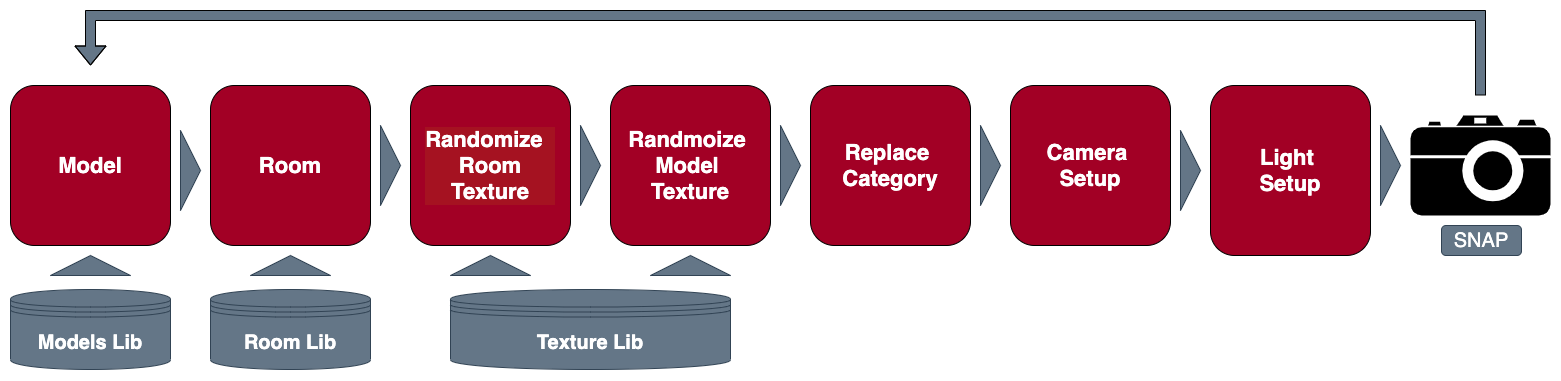
\includegraphics[width=\textwidth]{/Users/apple/OVGU/Thesis/code/3dReconstruction/report/images/concept/process}
    \caption{Automated pipeline for image generatiion with different blocks and external libraries.}
    \label{fig:pipline process}
\end{figure}

\subsection{Modes of operations}
Creation of dataset can either be automated or by manual intervention.
Automated images may not give us the perfect images which we expect.
There can be some bad lighting, unexpected intersections with other objects, unforseen camera angles, etc.
To facilitate ease of use for the user, the application has 3 key pipelines.

\begin{enumerate}
\item Single Room pipeline
\item Manual Room pipeline
\item Multi Objects pipeline
\end{enumerate}

Single Room pipeline is used to create the dataset with objects in the center of an empty room.
A room path can either be provided, else a default room is imported.
Manual Room pipeline randomises a furnished room, and then replaces the category under observation.
The selection of object to be replaced is also random.
In this mode, the user has the control over taking the snap of the scene.
The user can randomise model an room textures, randomise camera position or manually set it and randomise the lighting conditions.
Once the user is satisfied with the view of the scene, images can be saved with a click of the Snap button.
In Multi Objects pipeline, all the process mentioned in the Manual Room pipeline is automated.
The user won't have control over any of the process, while the program snaps images at random.
Another version of pipeline which is similar to Single Room pipeline is the Multi-threaded Single Room pipeline.
As the name suggests, multiple rooms are created based on the number of categories and for each room the Single Room pipeline is applied in parallel.
This is an attempt to let the tool perform faster with multi-threading.
The multi-process uses Coroutines which is still a sequential operation and hence this pipeline needs some work.
To our estimate even the Multi-threaded pipeline runs 1.5 times faster than Single room pipeline.

\subsection{Scenes from SceneNet}
For the rooms in our ersatz environments we utilize scenes provided by SceneNet ~\cite{McCormac:etal:ICCV2017}.
SceneNet has made 25 rooms available for public.
We only use scenes of type Bedroom(11), Kitchen(1), Living room(6) and office(7).
Figure ~\ref{fig:Scene Types} shows different types of scenes utilised to generate synthetic dataset.
These scenes are further modified by adding few more objects of categories present in Pix3D, so that we get more variations in the dataset.
The distribution of furnitures matching the category of Pix3D in the scenes are as shown in figrue ~\ref{fig:distribution of scenes}.
Each scene is replaced for every snap we take for the dataset we create at random.

\begin{figure}[!ht]
    \centering
    \subfloat[][]{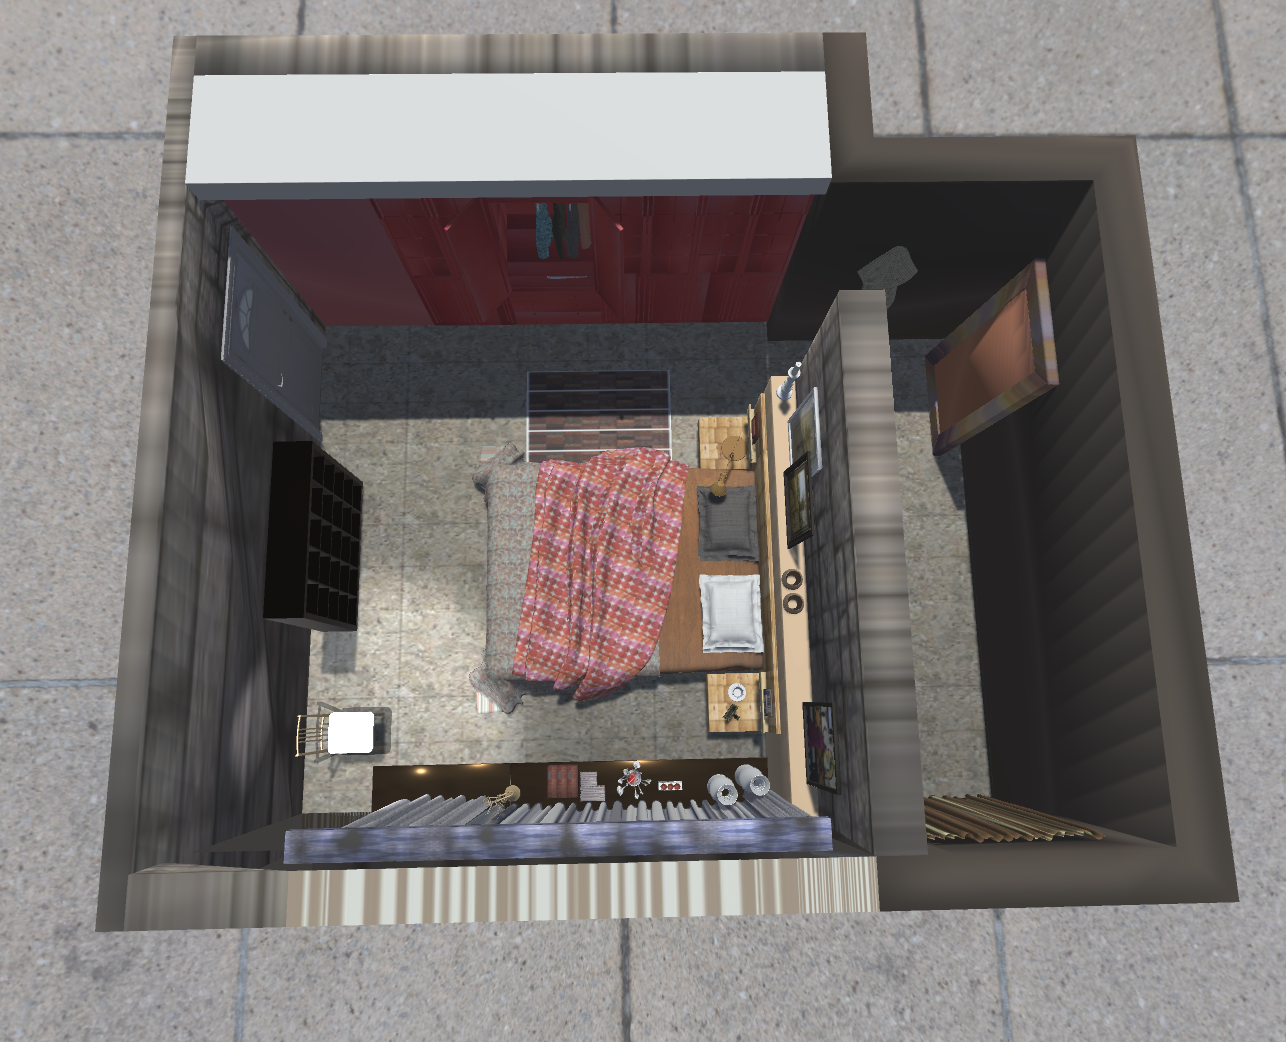
\includegraphics[width=.35\textwidth, height = .35\textwidth]{/Users/apple/OVGU/Thesis/code/3dReconstruction/report/images/implementation/scenenet_scenes/scene_bedroom}}\quad
    \subfloat[][]{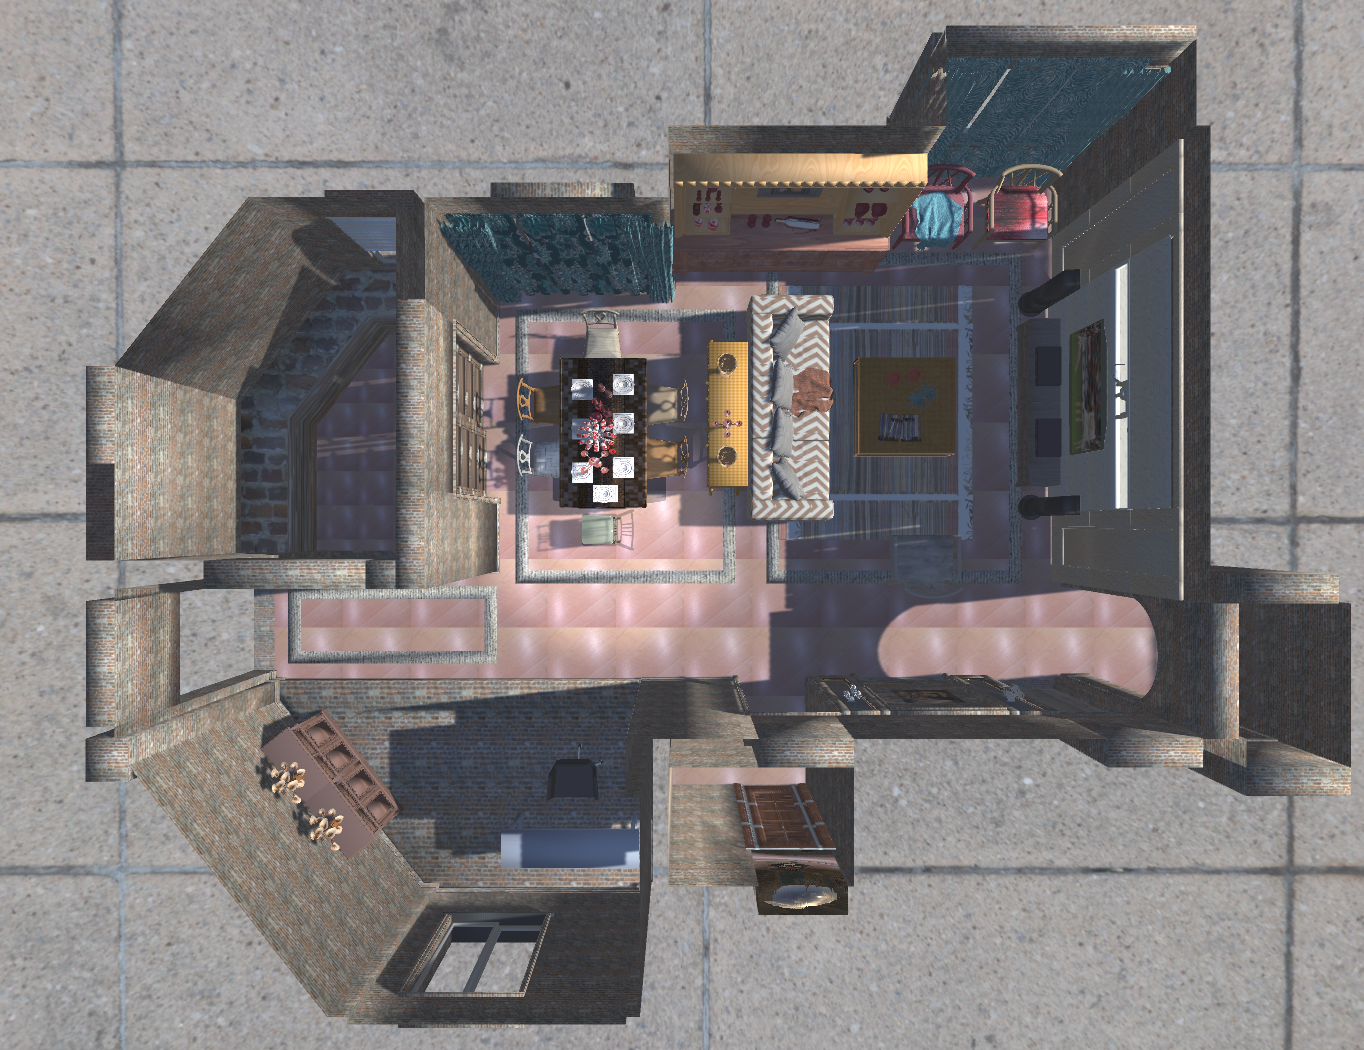
\includegraphics[width=.35\textwidth, height = .35\textwidth]{/Users/apple/OVGU/Thesis/code/3dReconstruction/report/images/implementation/scenenet_scenes/scene_livingroom}}\\
    \subfloat[][]{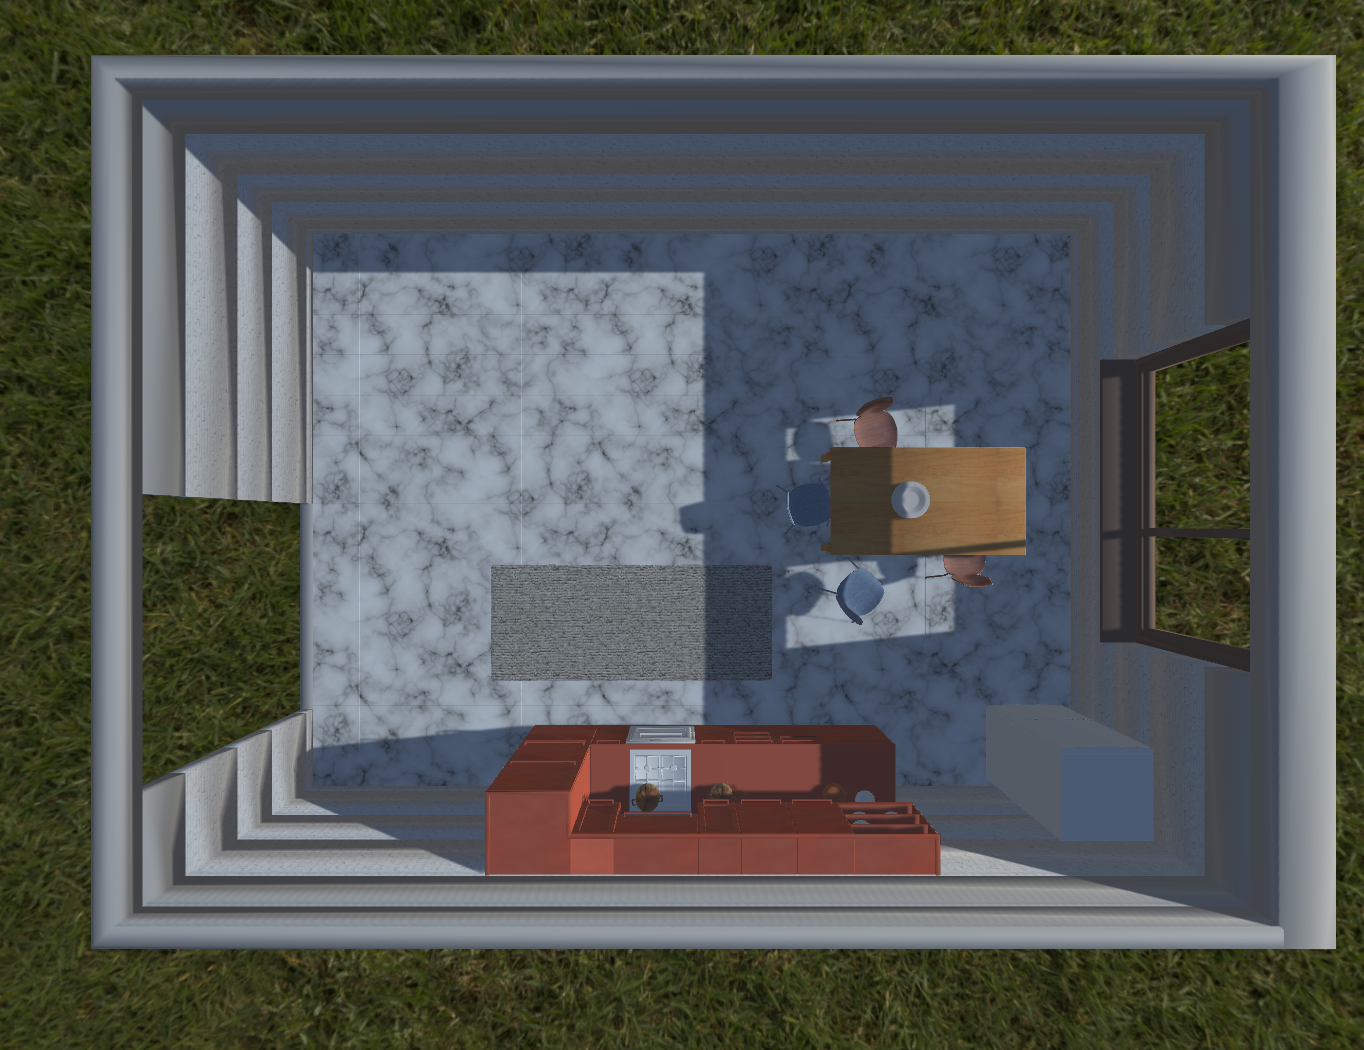
\includegraphics[width=.35\textwidth, height = .35\textwidth]{/Users/apple/OVGU/Thesis/code/3dReconstruction/report/images/implementation/scenenet_scenes/scene_kitchen}}\quad
    \subfloat[][]{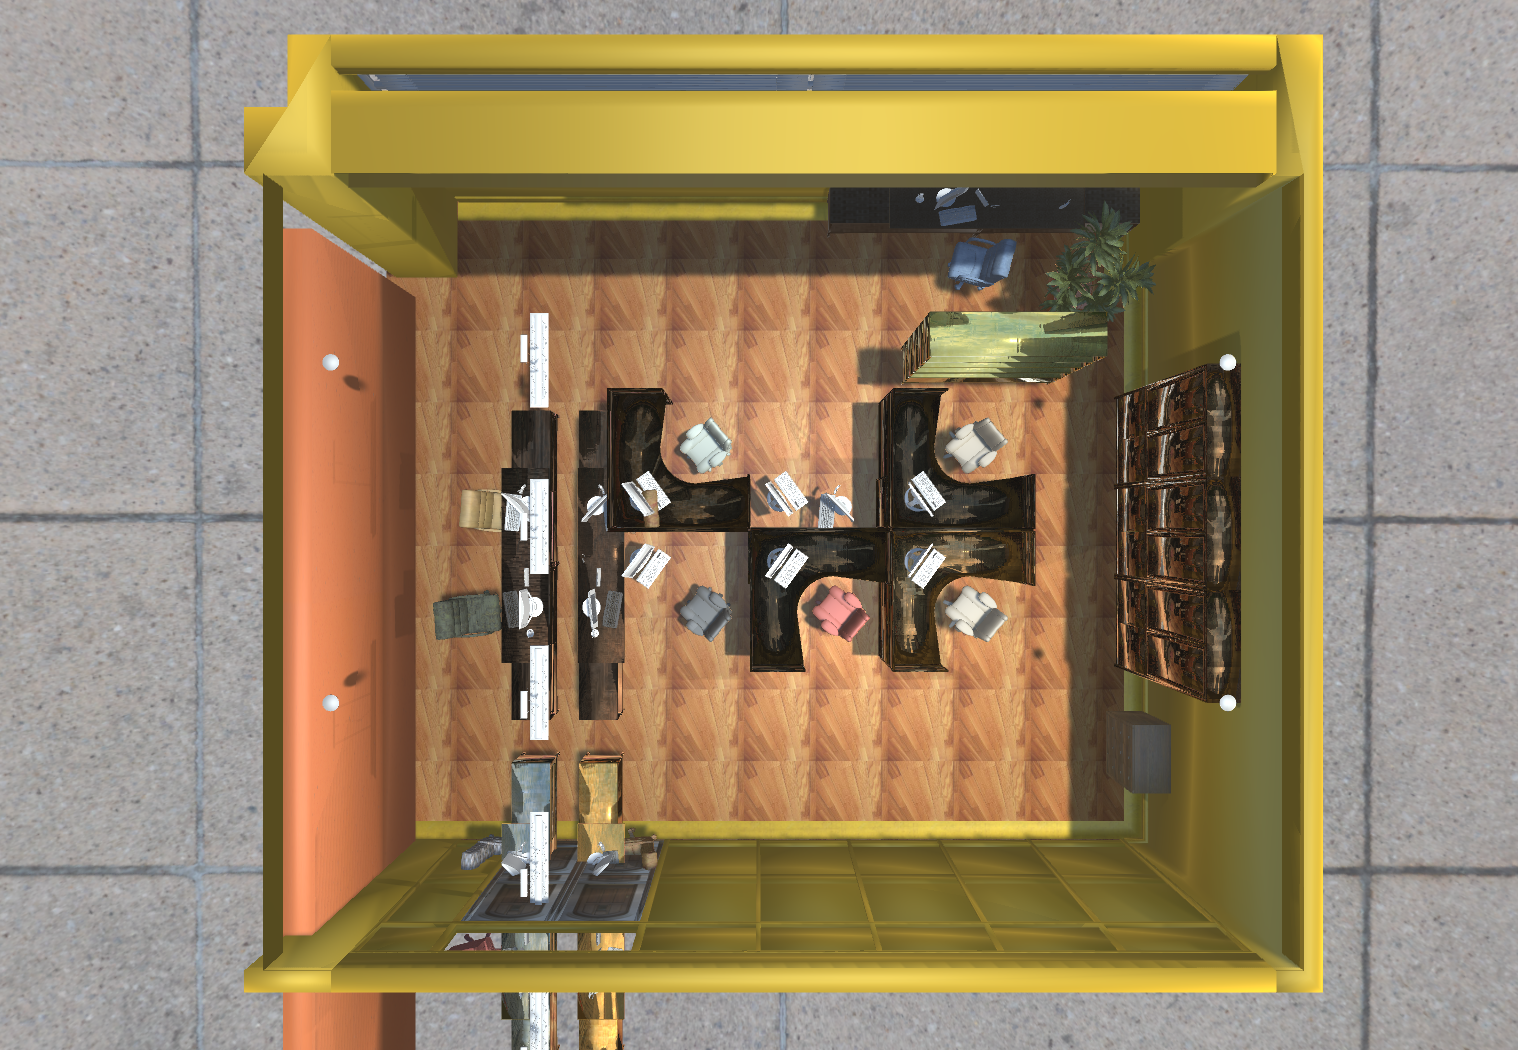
\includegraphics[width=.35\textwidth, height = .35\textwidth]{/Users/apple/OVGU/Thesis/code/3dReconstruction/report/images/implementation/scenenet_scenes/scene_office}}
    \caption{Sample scene layouts from SceneNet. Types: (a)Bedroom, (b)LivingRoom, (c)Kitchen and (d)Office}
    \label{fig:Scene Types}
\end{figure}

\begin{figure}[!ht]
    \centering
    \subfloat[][]{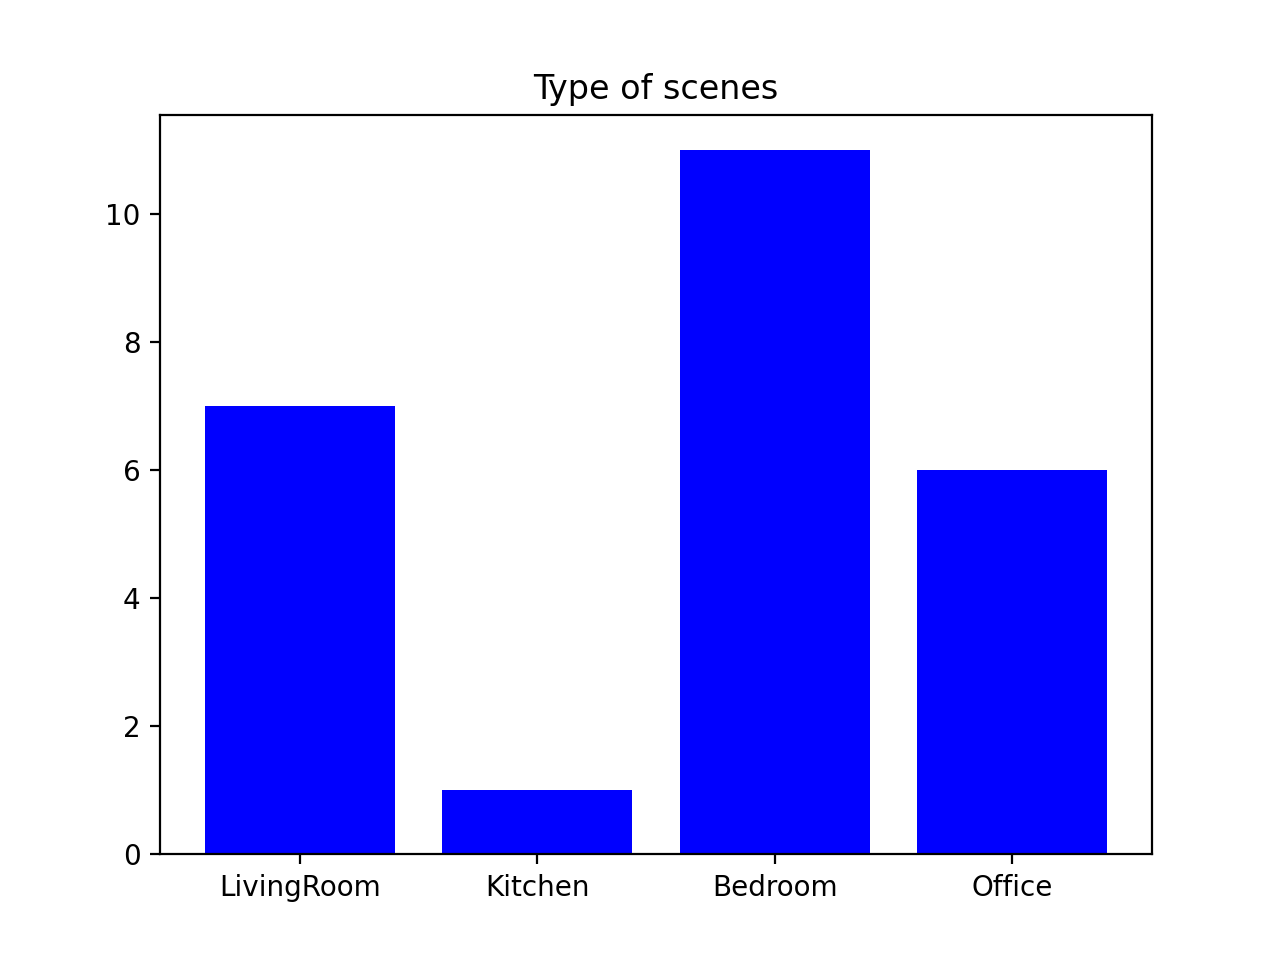
\includegraphics[width=.45\textwidth,height=6cm]{/Users/apple/OVGU/Thesis/code/3dReconstruction/report/images/implementation/scenenet_scenes/types_of_scenes}}\quad
    \subfloat[][]{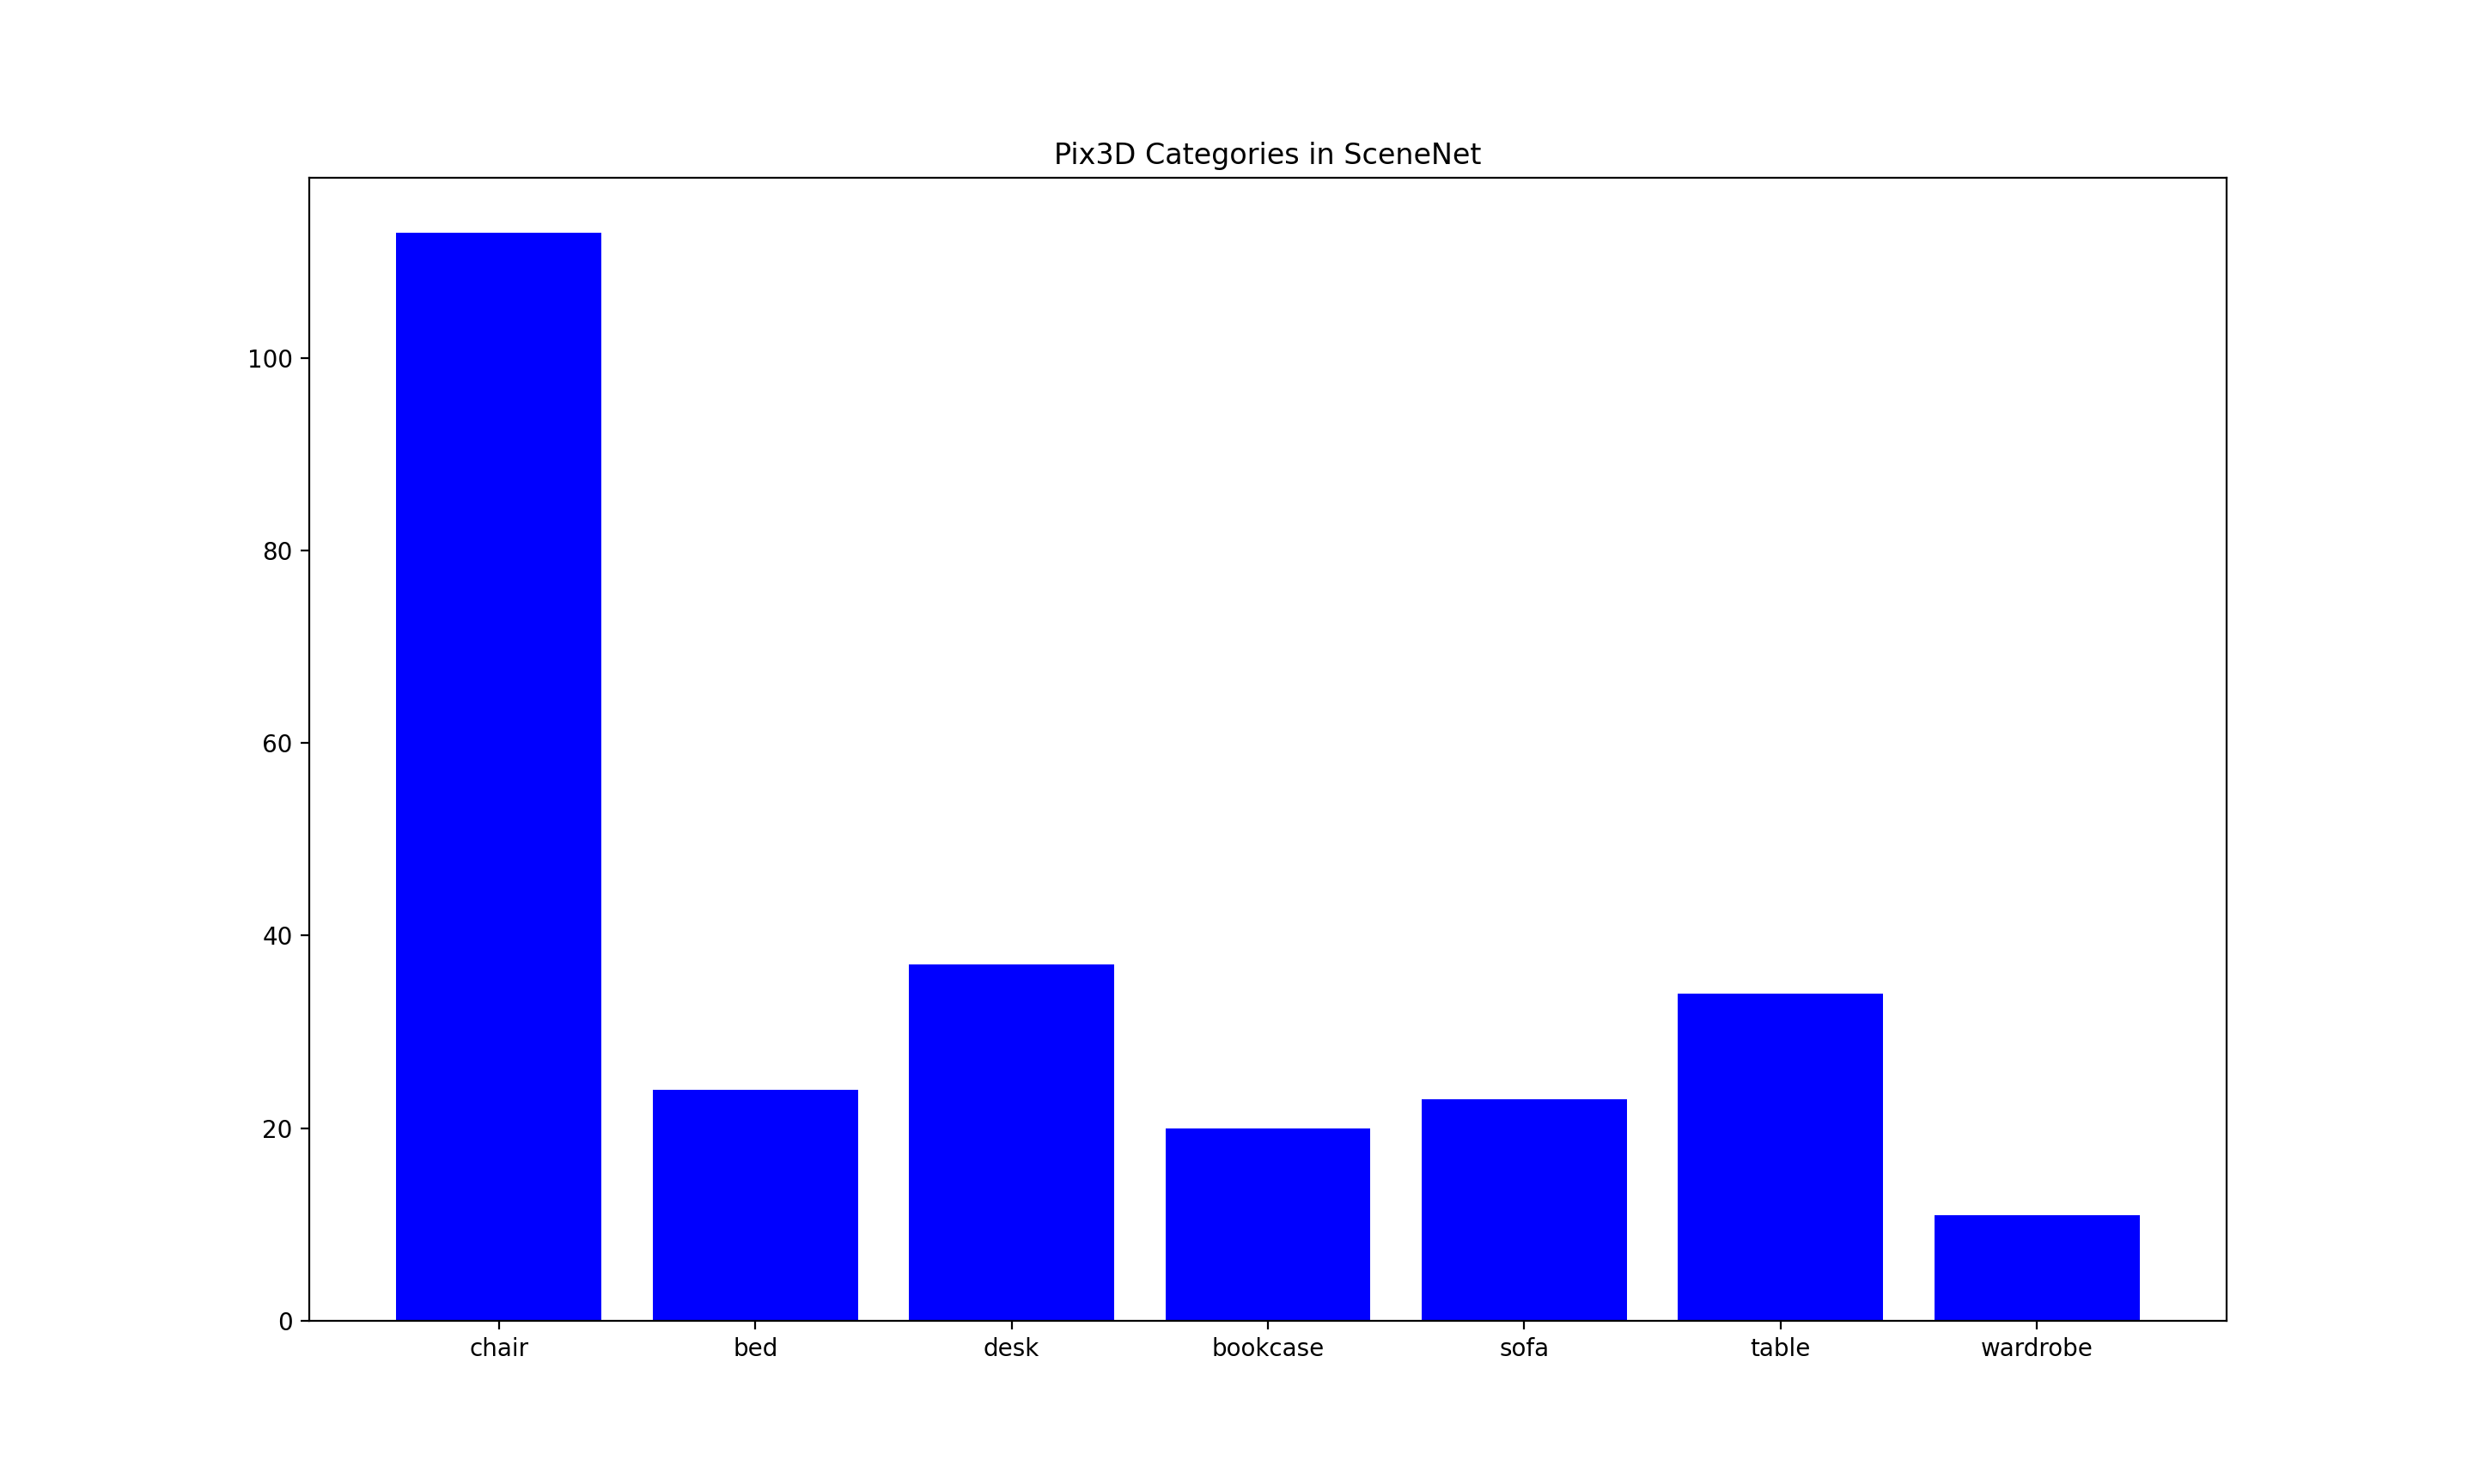
\includegraphics[width=.45\textwidth,height=6cm]{/Users/apple/OVGU/Thesis/code/3dReconstruction/report/images/implementation/scenenet_scenes/distribution_categories_scenenet}}\\
    \caption{(a)Distribution of types ofs scenes, (b) Distribution of objects matching the categories of pix3d in scenes}
    \label{fig:distribution of scenes}
\end{figure}

\subsection{Camera ViewPoints}

The distance of camera from the target object is a configurable entity.
The user can set the minimum and maximum distance to the target object for the camera to be placed.
The program will then randomly select a point within this range.
Similarly the height of the camera can be configured by the user.
The camera is programed to always look towards the target object and will be changed if the object is not in the frame.
This is acheived by passing a ray and determining if the center of the target object is visible.
To make the frame realistic, we avoid unrelatable views by applying a constraint on the camera poisiton and make sure that the camera is in front of the target object within an angle of 60 degrees.
Figure ~\ref{fig:Camera viewpoints} shows samples of different camera view points on a constant object and scene.

\begin{figure}
    \centering
    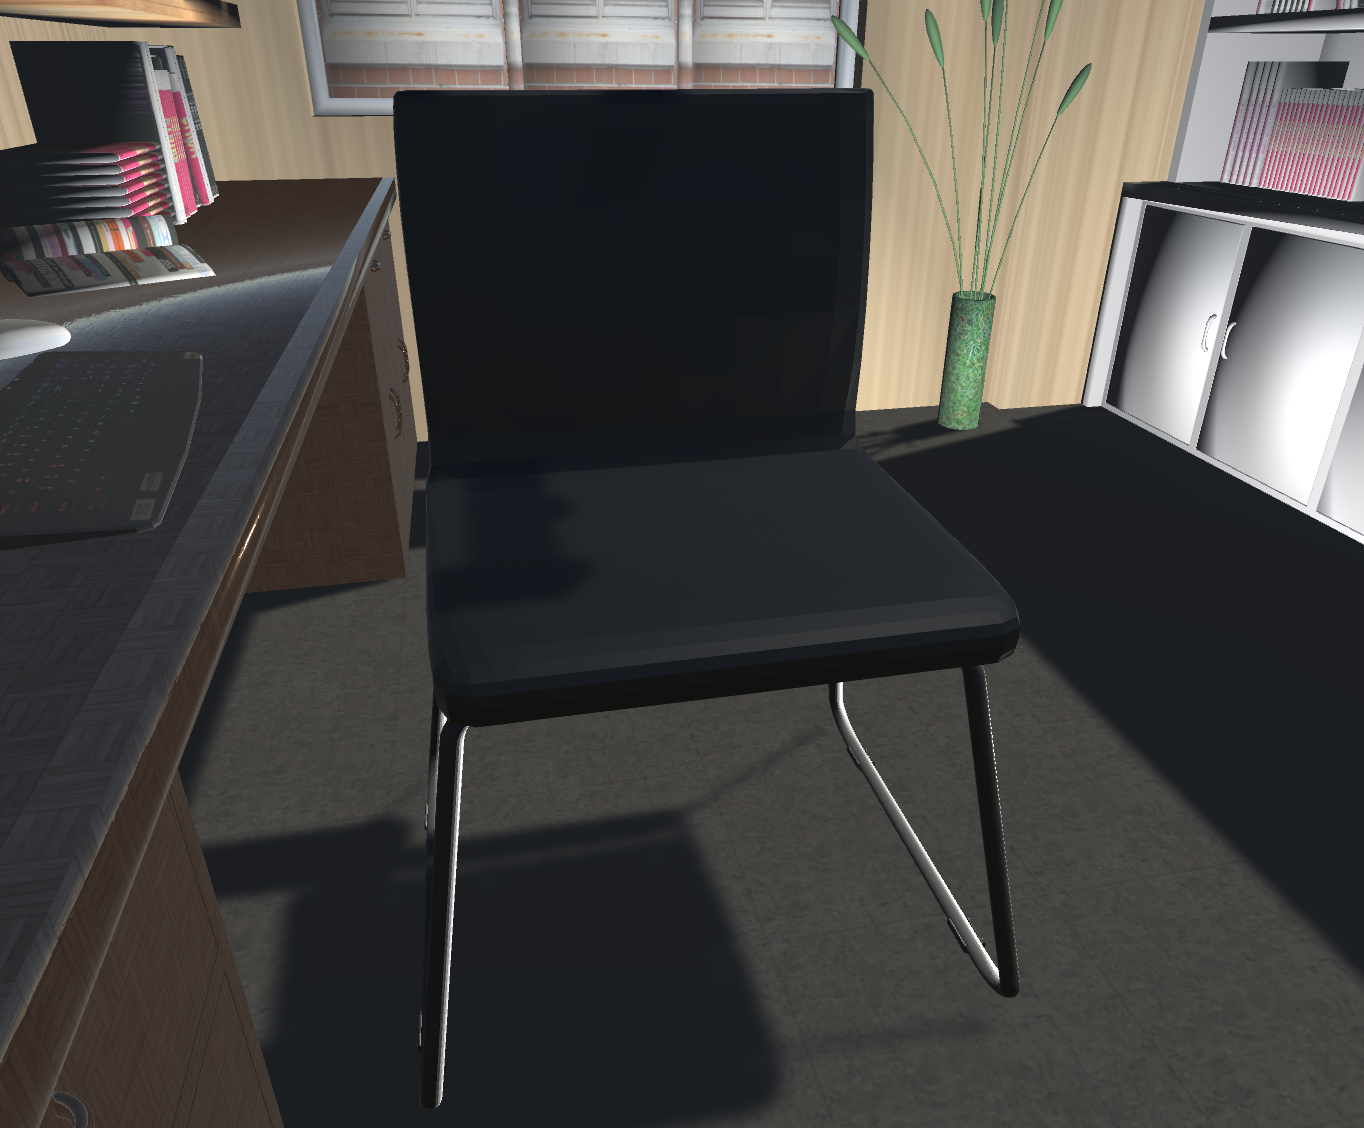
\includegraphics[width=.4\textwidth, height = .3\textwidth,valign=m]{/Users/apple/OVGU/Thesis/code/3dReconstruction/report/images/implementation/randomisation/camera1}
    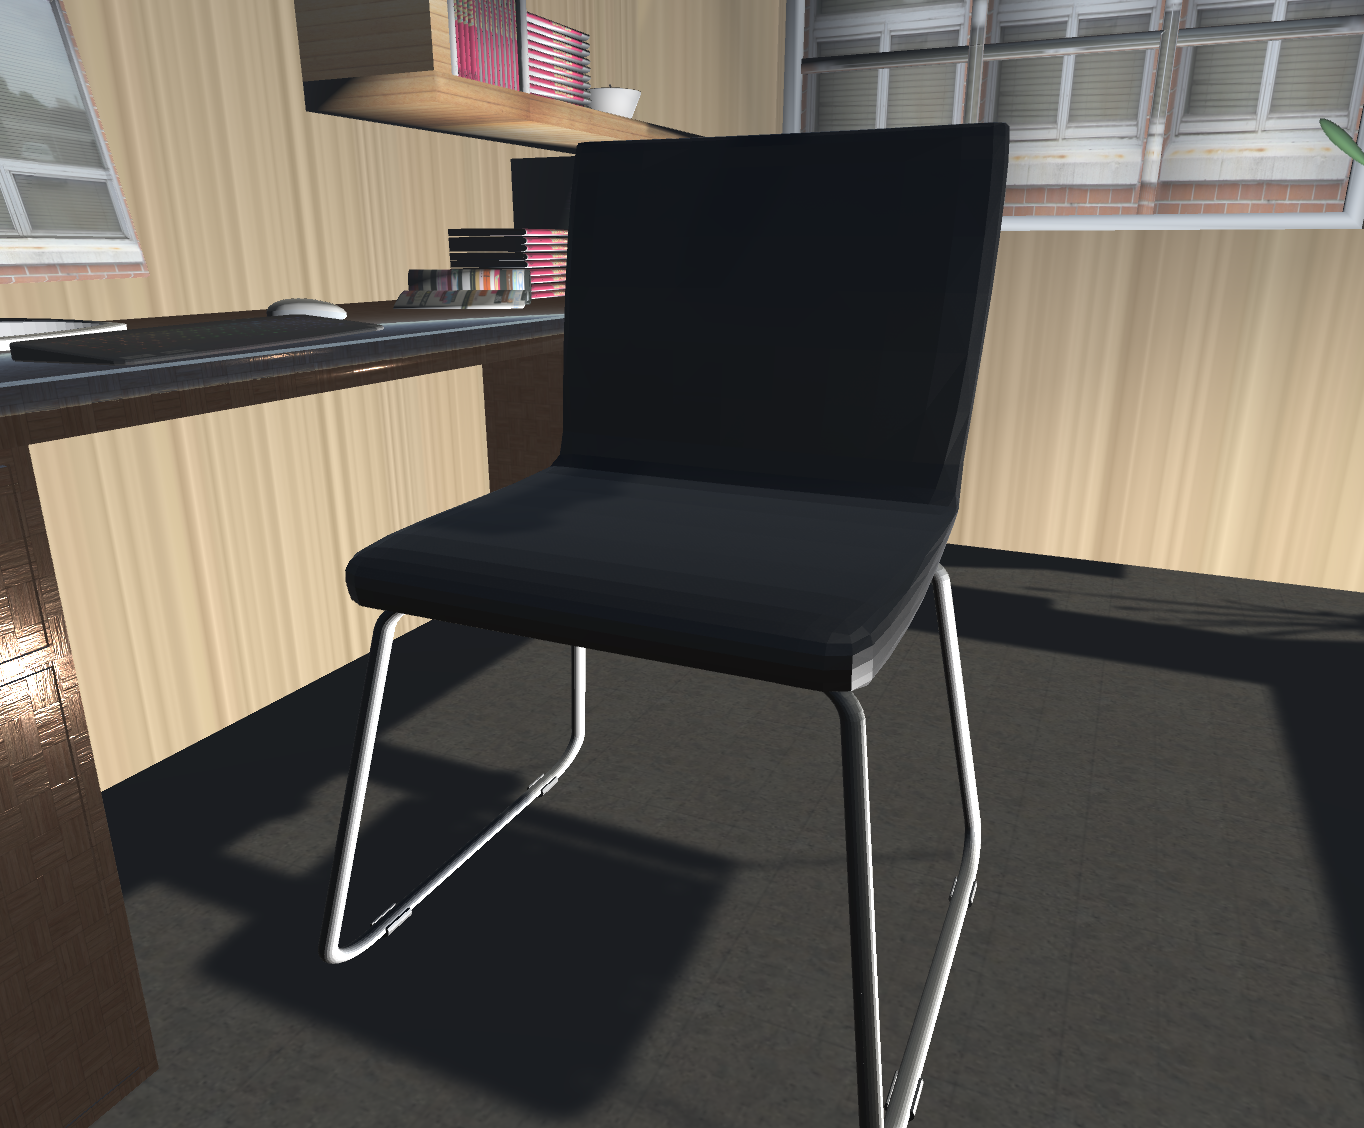
\includegraphics[width=.4\textwidth, height = .3\textwidth,valign=m]{/Users/apple/OVGU/Thesis/code/3dReconstruction/report/images/implementation/randomisation/camera2}\\
    \vspace{0.1cm}
    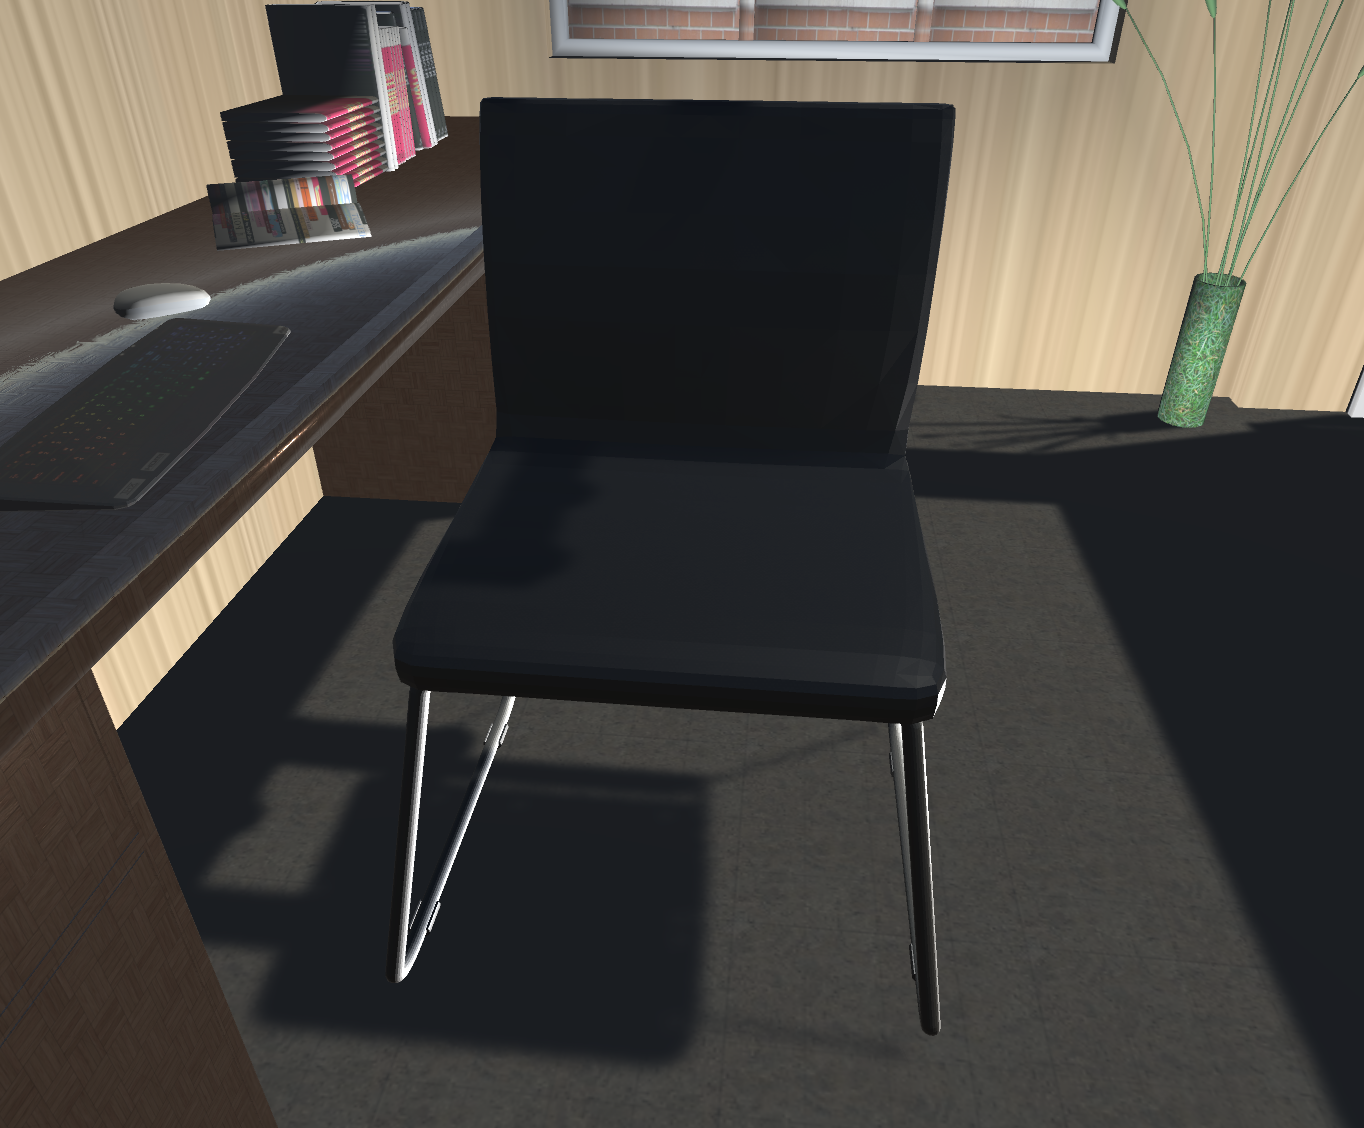
\includegraphics[width=.4\textwidth, height = .3\textwidth,valign=m]{/Users/apple/OVGU/Thesis/code/3dReconstruction/report/images/implementation/randomisation/camera3}
    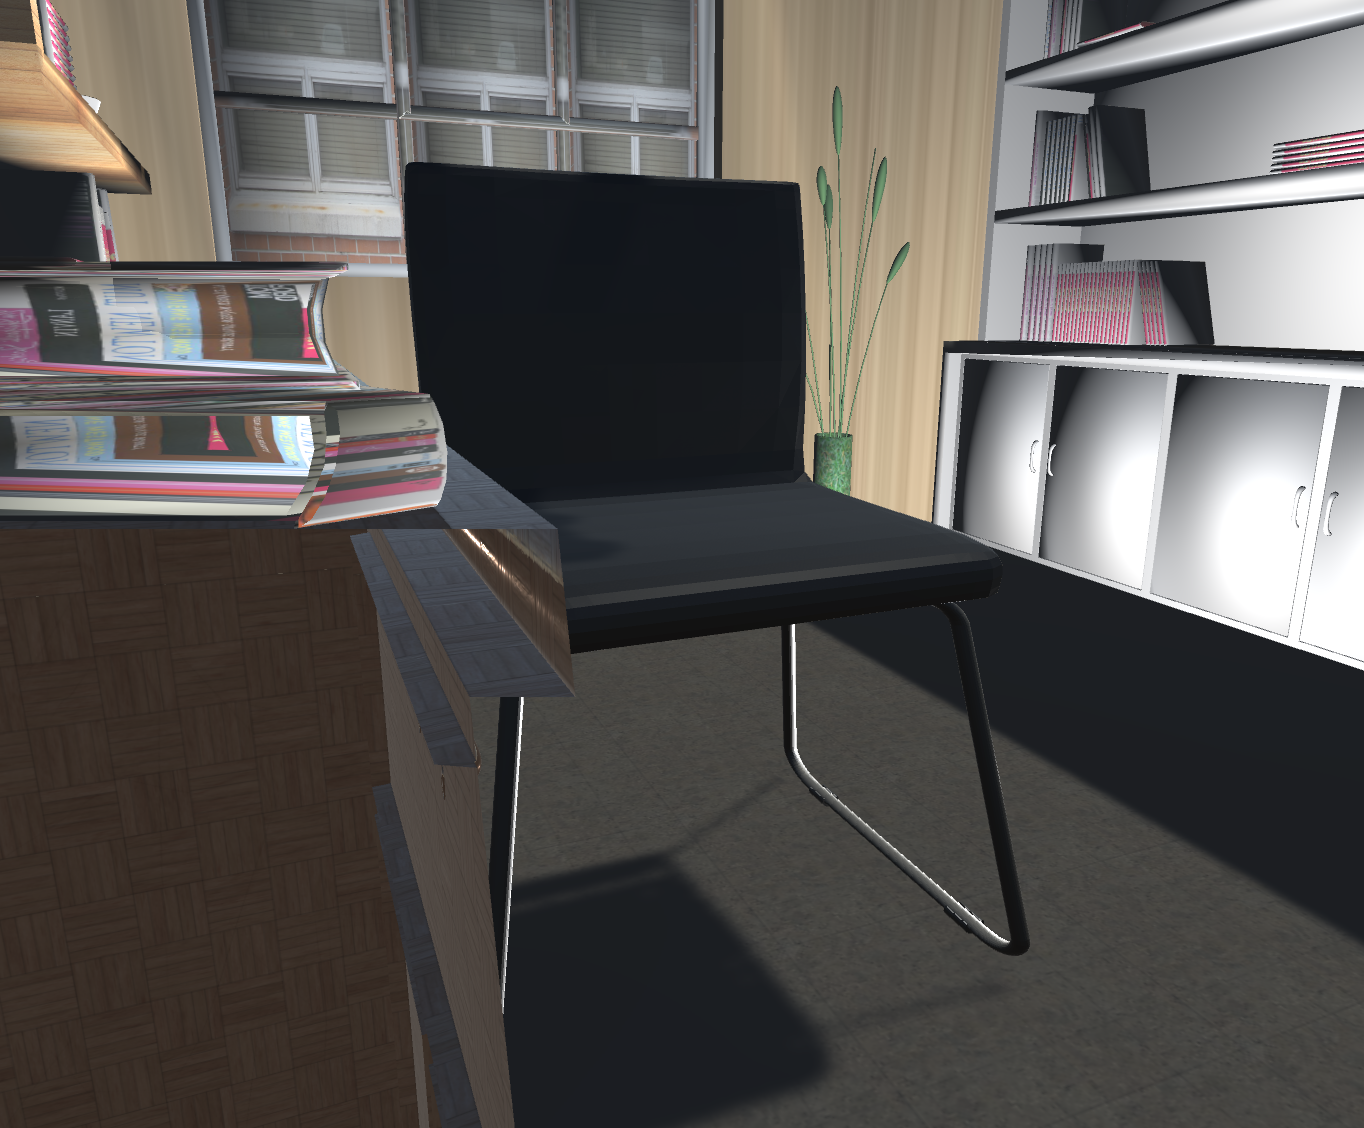
\includegraphics[width=.4\textwidth, height = .3\textwidth,valign=m]{/Users/apple/OVGU/Thesis/code/3dReconstruction/report/images/implementation/randomisation/camera4}\\
    \caption{Sample images with different camera viewpoints of same object with a constant scene.}
    \label{fig:Camera viewpoints}
\end{figure}

\subsection{Lightings and Shadows}

We consider lighting to be a key component of the photorealism.
The shadows formed with different lighting condition enhance the photorealism of the images.
For this purpose we use 3 types of lights offered in Unity.

\begin{itemize}
    \item Point light
    \item Spot light
    \item Sunlight
\end{itemize}

Point lights act as indoor lights for the room the range of which can be varied.
We pre-define 6 light patterns for a room with cuboid shape.
Knowing the bounds of the room we decide how to place the lights by randomly select 1 to 6 lights with corresponding light patterns on the ceiling.
For the spotlight, only a single light is placed a meter above the target object.
This light gives a variation which focuses only on the target object.
Both point and spot-light have color variation along with varing brightness.
Sunlight is the default light settings in Unity.
This is specifically effective when the room has windows forming more realistic shadows.
In this case, we modulate the brightness and the angle at which the rays are emitted, which simulates different times of the day.
Additional to these different types of light, we give ceilings the property of light with limited brightness as we observed that the entire room does not lit up for single light source.
This is similar to what BlenderProc ~\cite{denninger2019blenderproc} does for all scenarios.
Samples of different lighting condition and shadows with varying color is displayed in figure ~\ref{fig:Lighting and shadows}.

Another randomised entity is the skybox.
Skybox acts as the outdoor scene for a given room.
For each of the pipeline, skybox changes for every snap taken.
This simulates different outdoor places and weather scenarios, thus providing more randomisation for rooms have open doors and windows.
Samples for different skyboxes are as shown in figure ~\ref{fig:skybox samples}.

%\begin{figure}
%    \centering
%    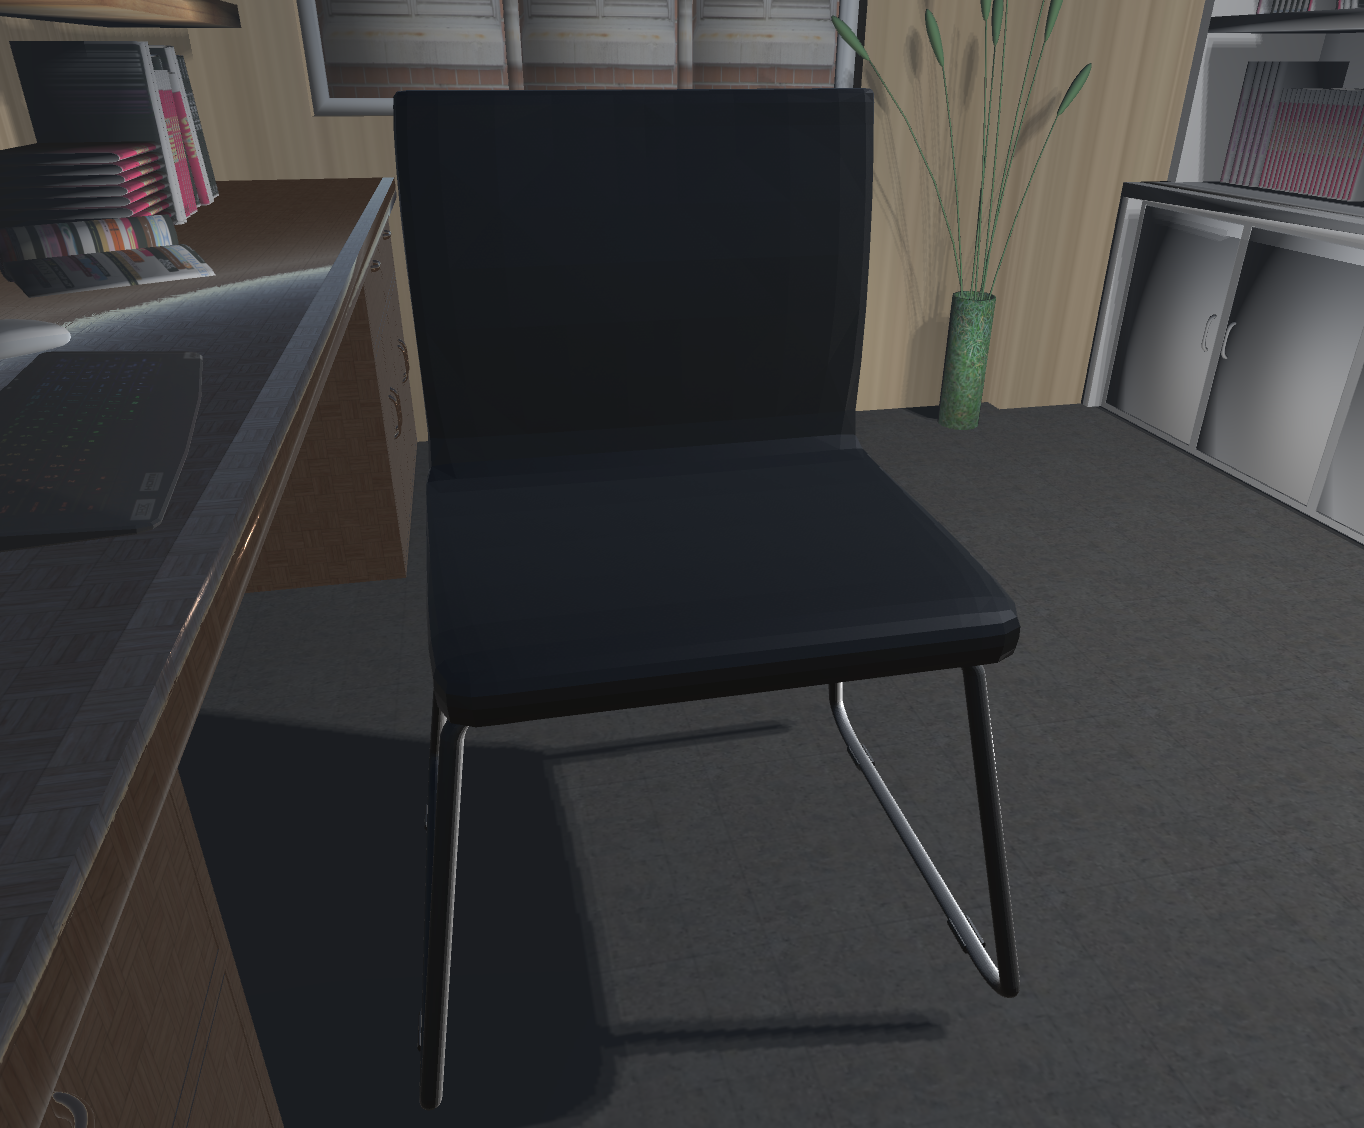
\includegraphics[width=.3\textwidth, height = .3\textwidth,valign=m]{/Users/apple/OVGU/Thesis/code/3dReconstruction/report/images/implementation/randomisation/lighting1}
%    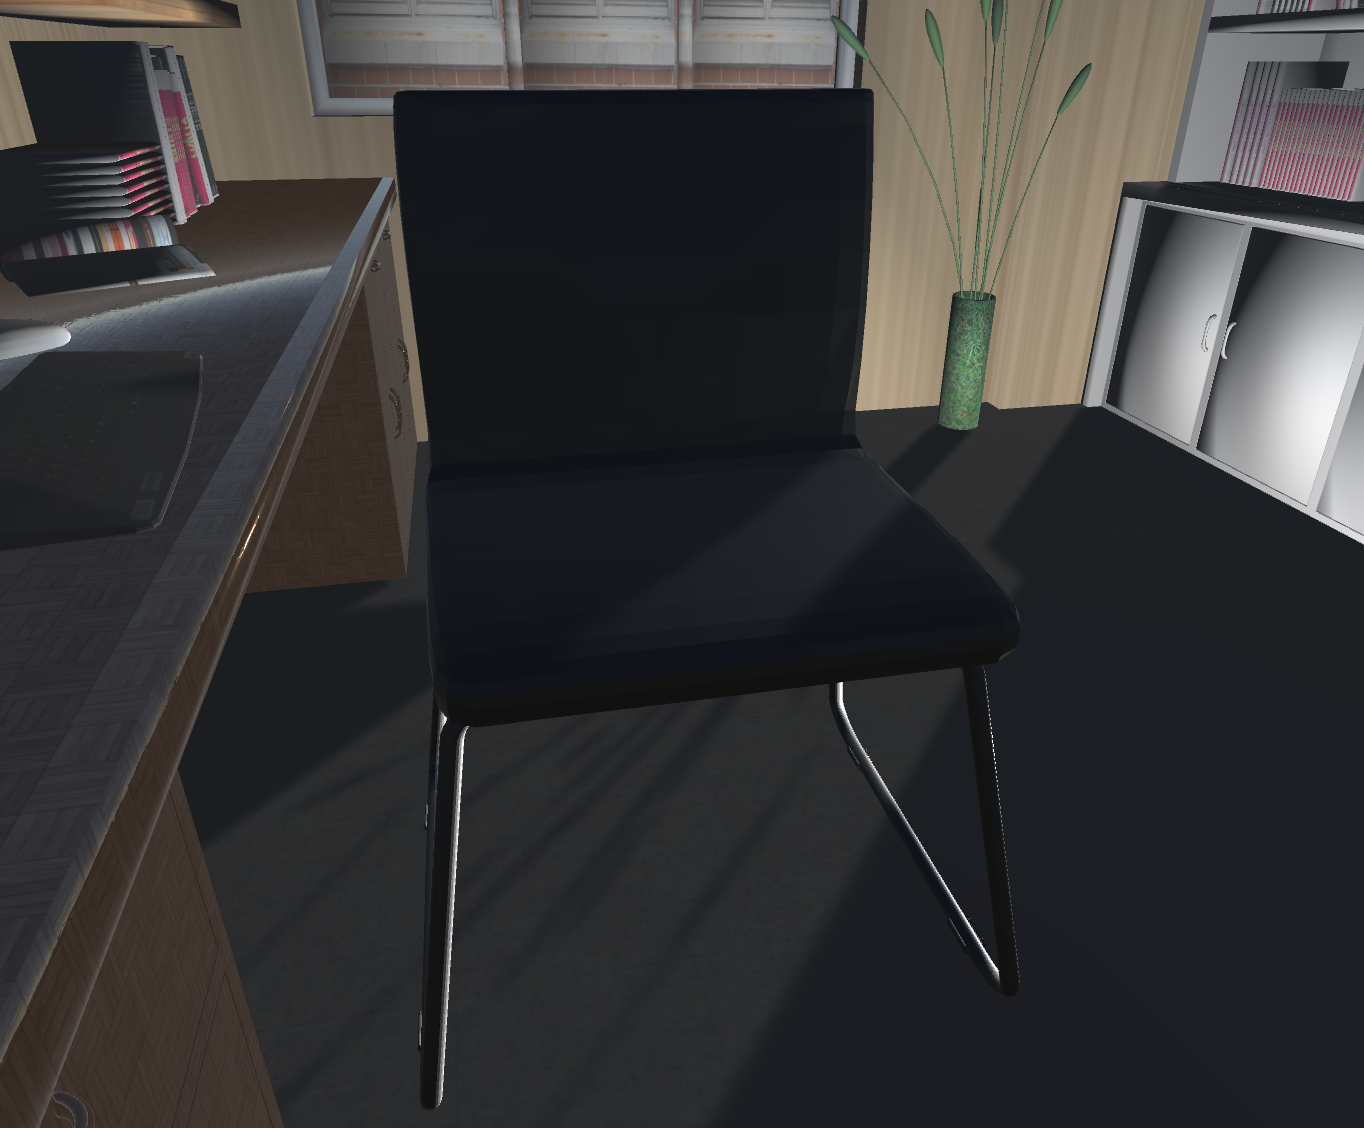
\includegraphics[width=.3\textwidth, height = .3\textwidth,valign=m]{/Users/apple/OVGU/Thesis/code/3dReconstruction/report/images/implementation/randomisation/lighting2}\\
%    \vspace{0.1cm}
%    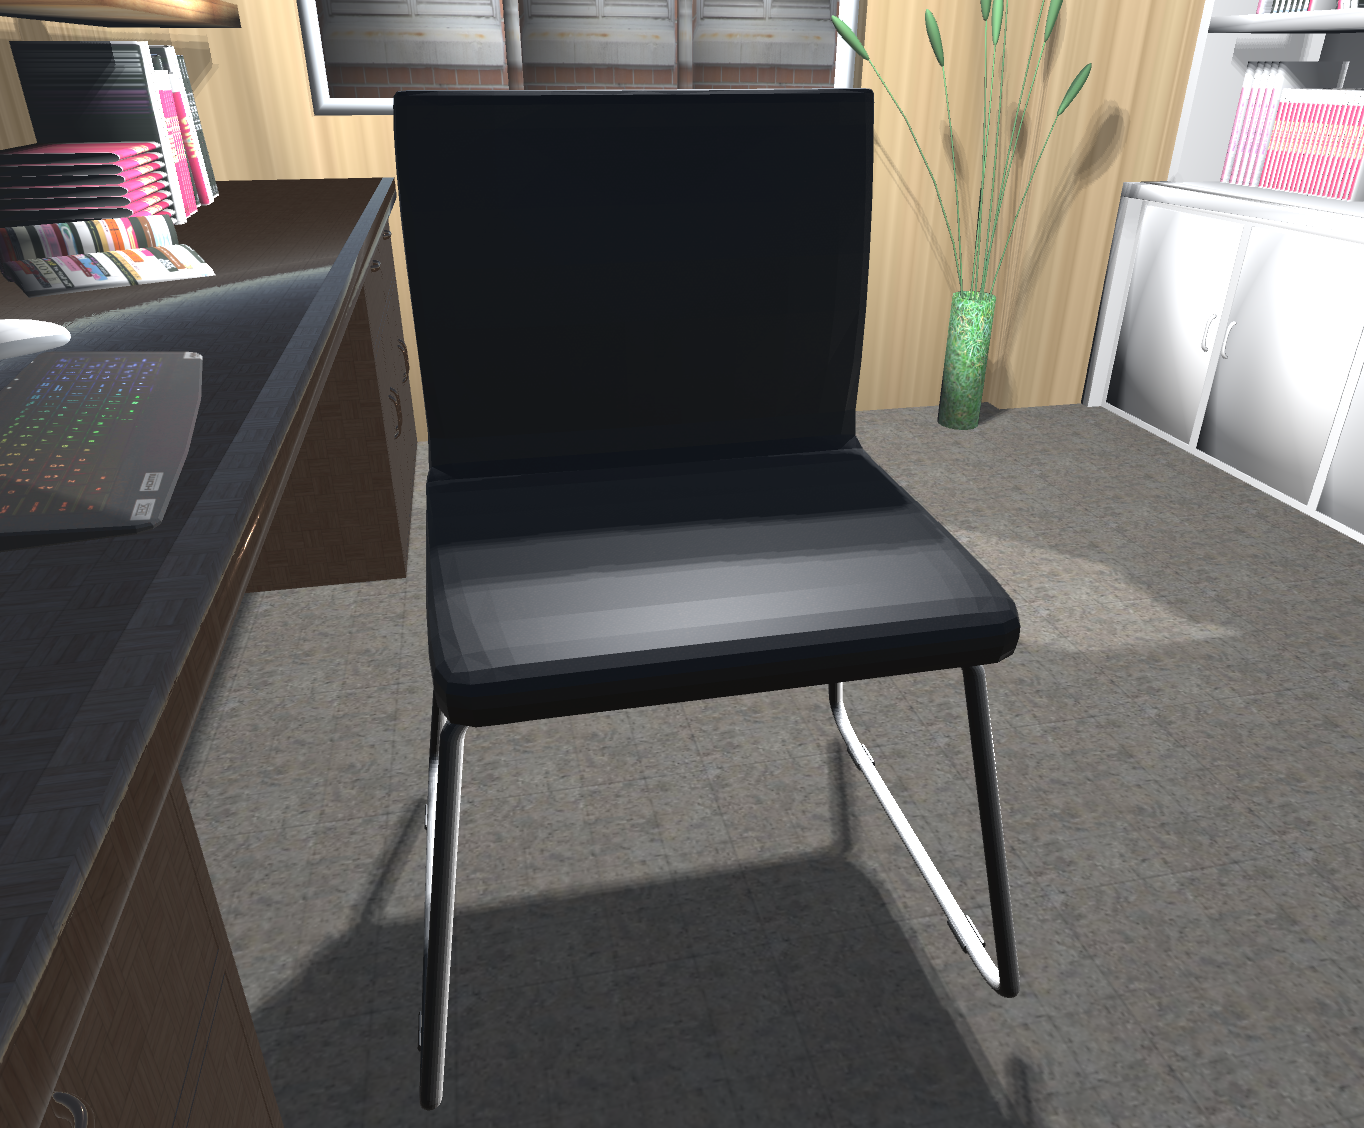
\includegraphics[width=.3\textwidth, height = .3\textwidth,valign=m]{/Users/apple/OVGU/Thesis/code/3dReconstruction/report/images/implementation/randomisation/lighting3}
%    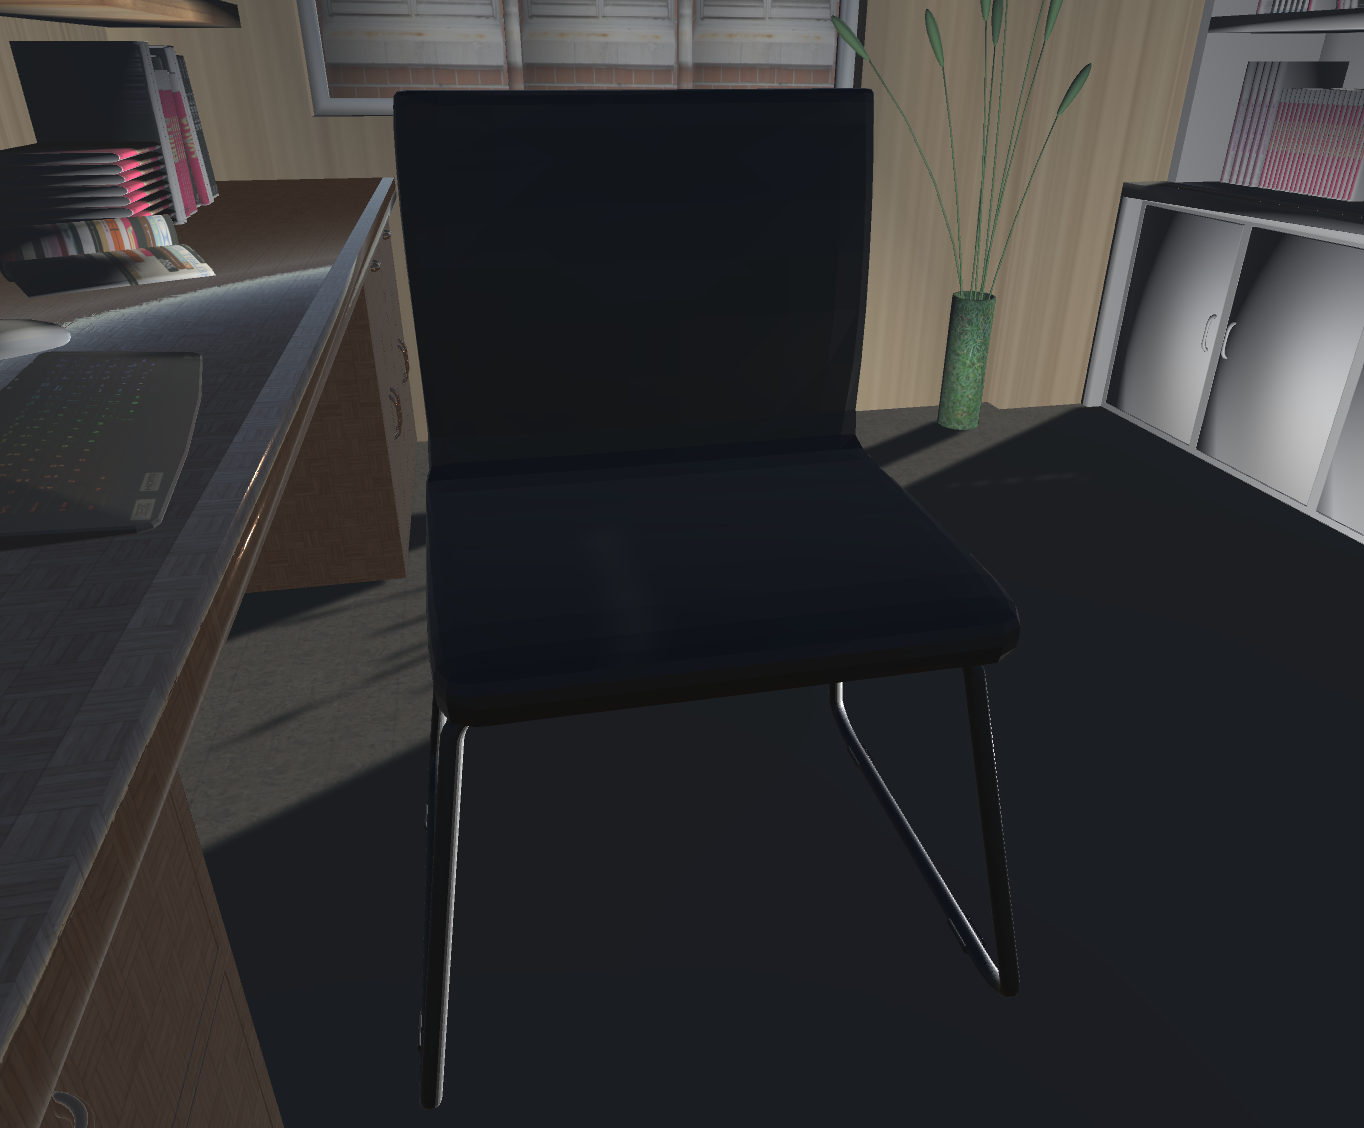
\includegraphics[width=.3\textwidth, height = .3\textwidth,valign=m]{/Users/apple/OVGU/Thesis/code/3dReconstruction/report/images/implementation/randomisation/lighting4}\\
%    \caption{Sample images with different lighting and shadows conditions}
%    \label{fig:Lighting and shadows}
%\end{figure}

\begin{figure}
    \centering
        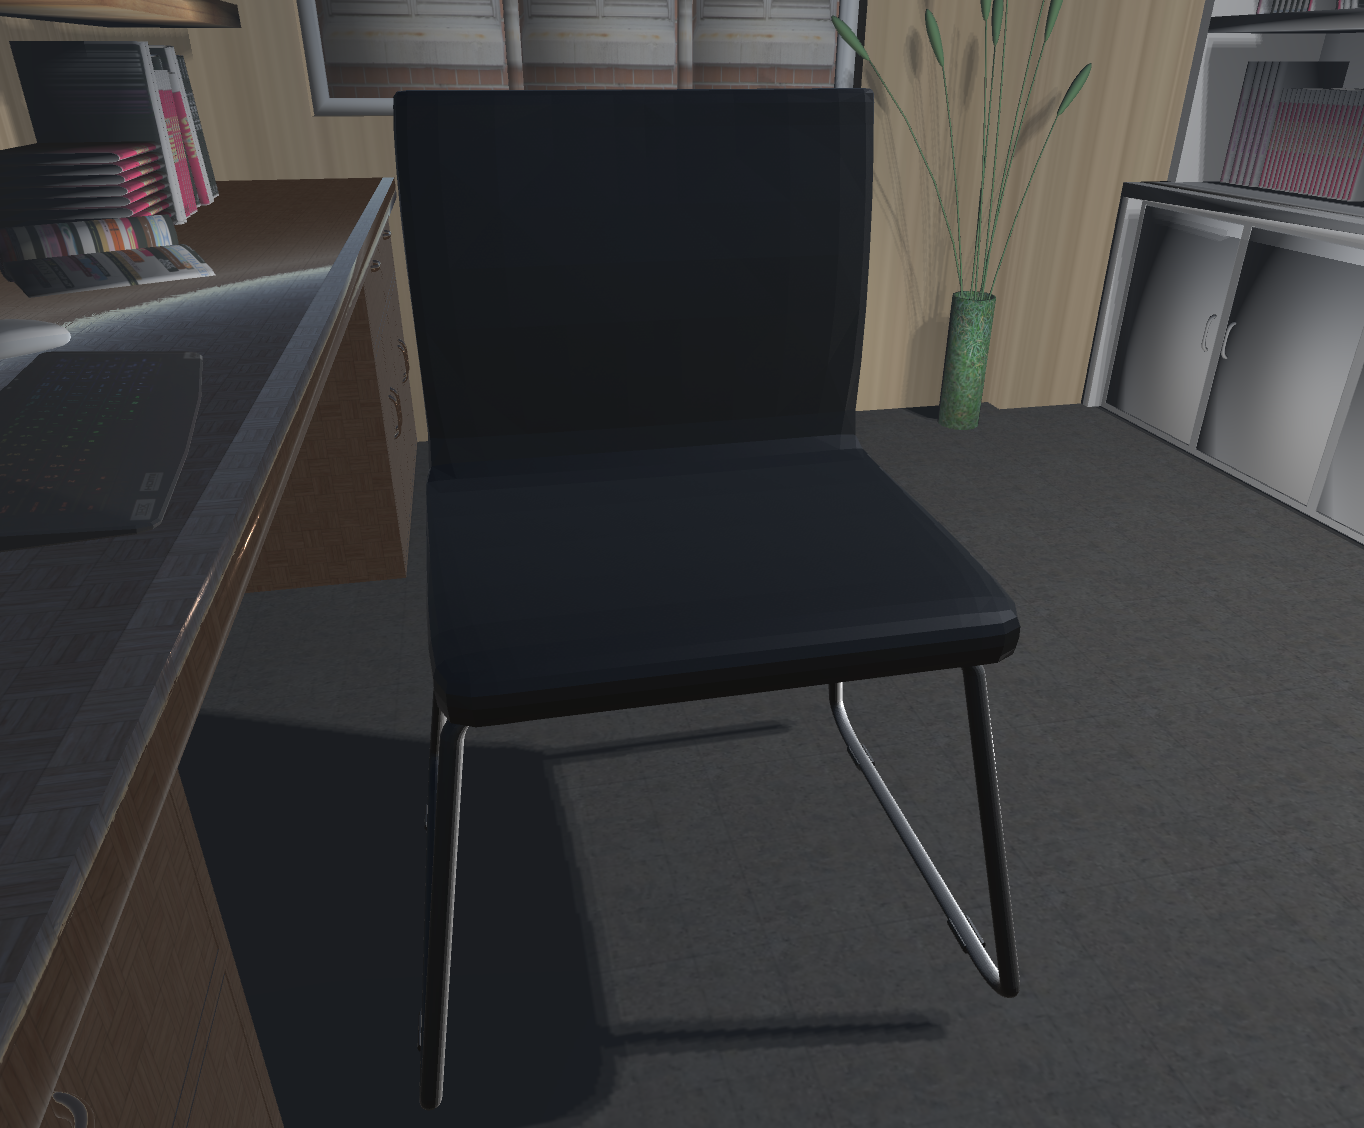
\includegraphics[width=.24\linewidth,valign=m]{/Users/apple/OVGU/Thesis/code/3dReconstruction/report/images/implementation/randomisation/lighting1}
        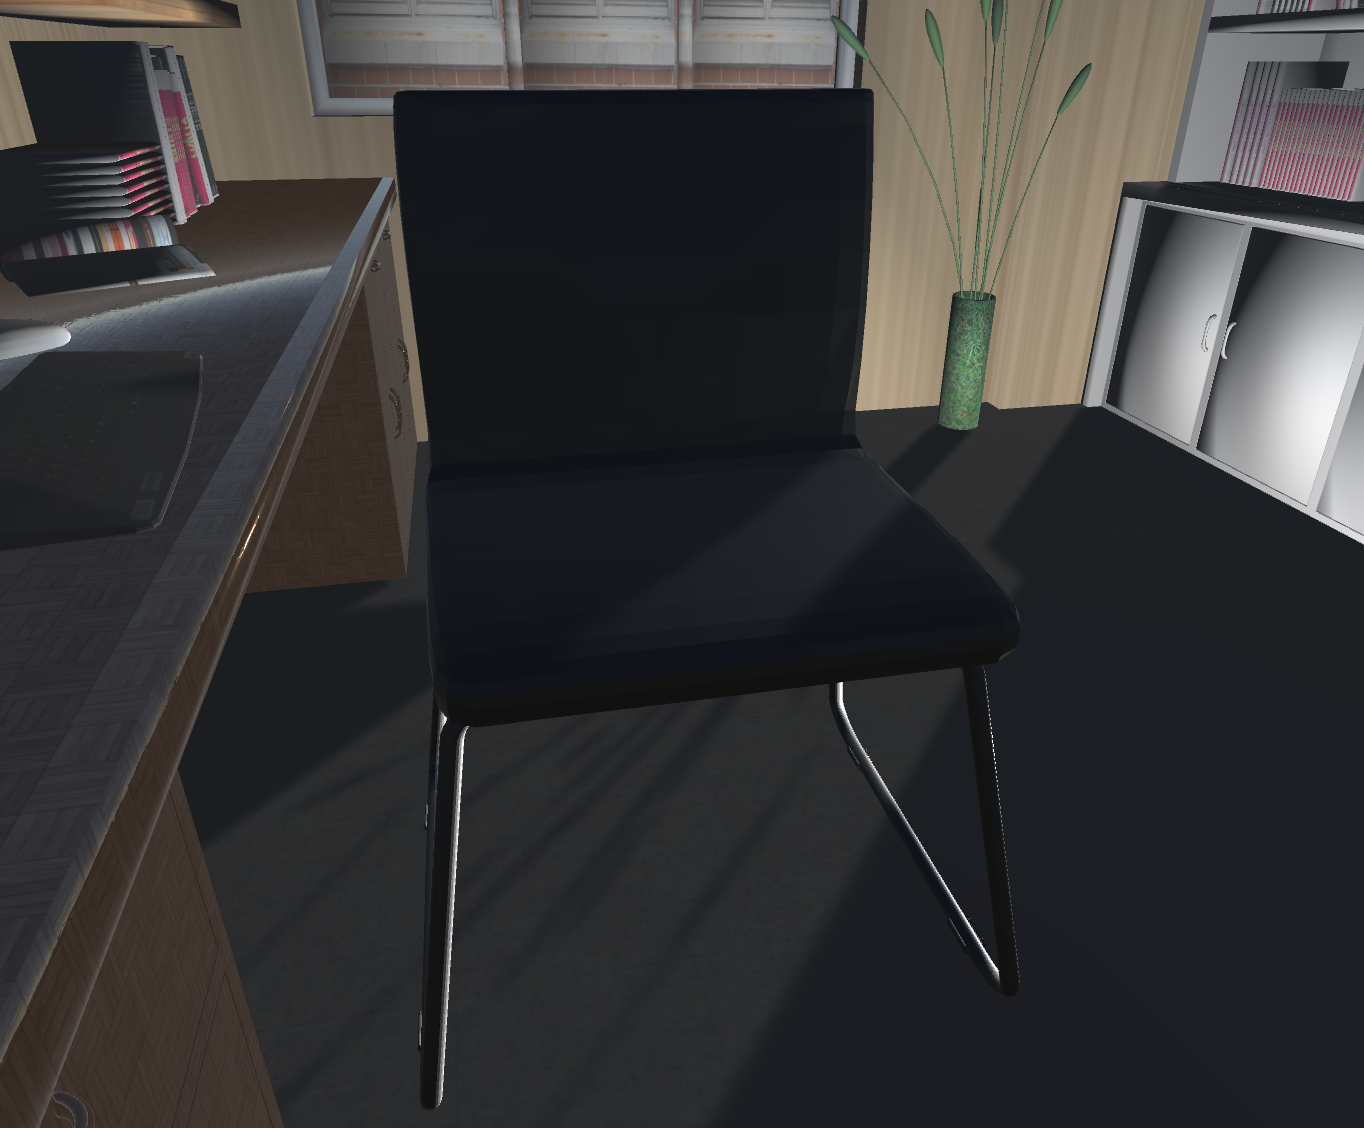
\includegraphics[width=.24\linewidth,valign=m]{/Users/apple/OVGU/Thesis/code/3dReconstruction/report/images/implementation/randomisation/lighting2}
        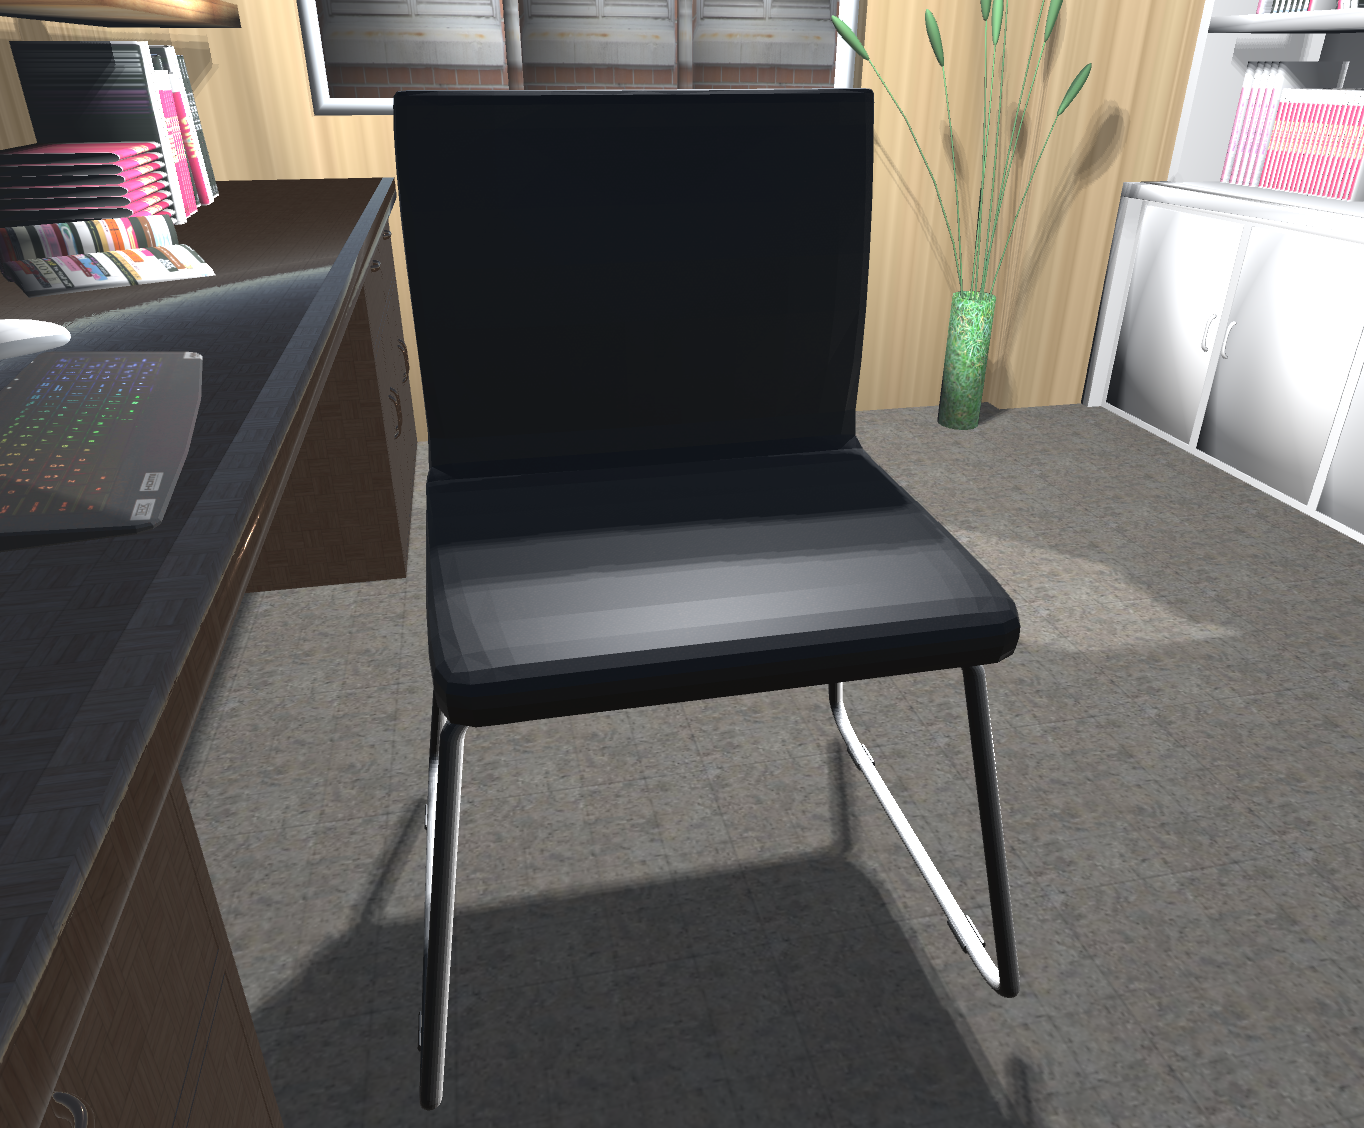
\includegraphics[width=.24\linewidth,valign=m]{/Users/apple/OVGU/Thesis/code/3dReconstruction/report/images/implementation/randomisation/lighting3}
        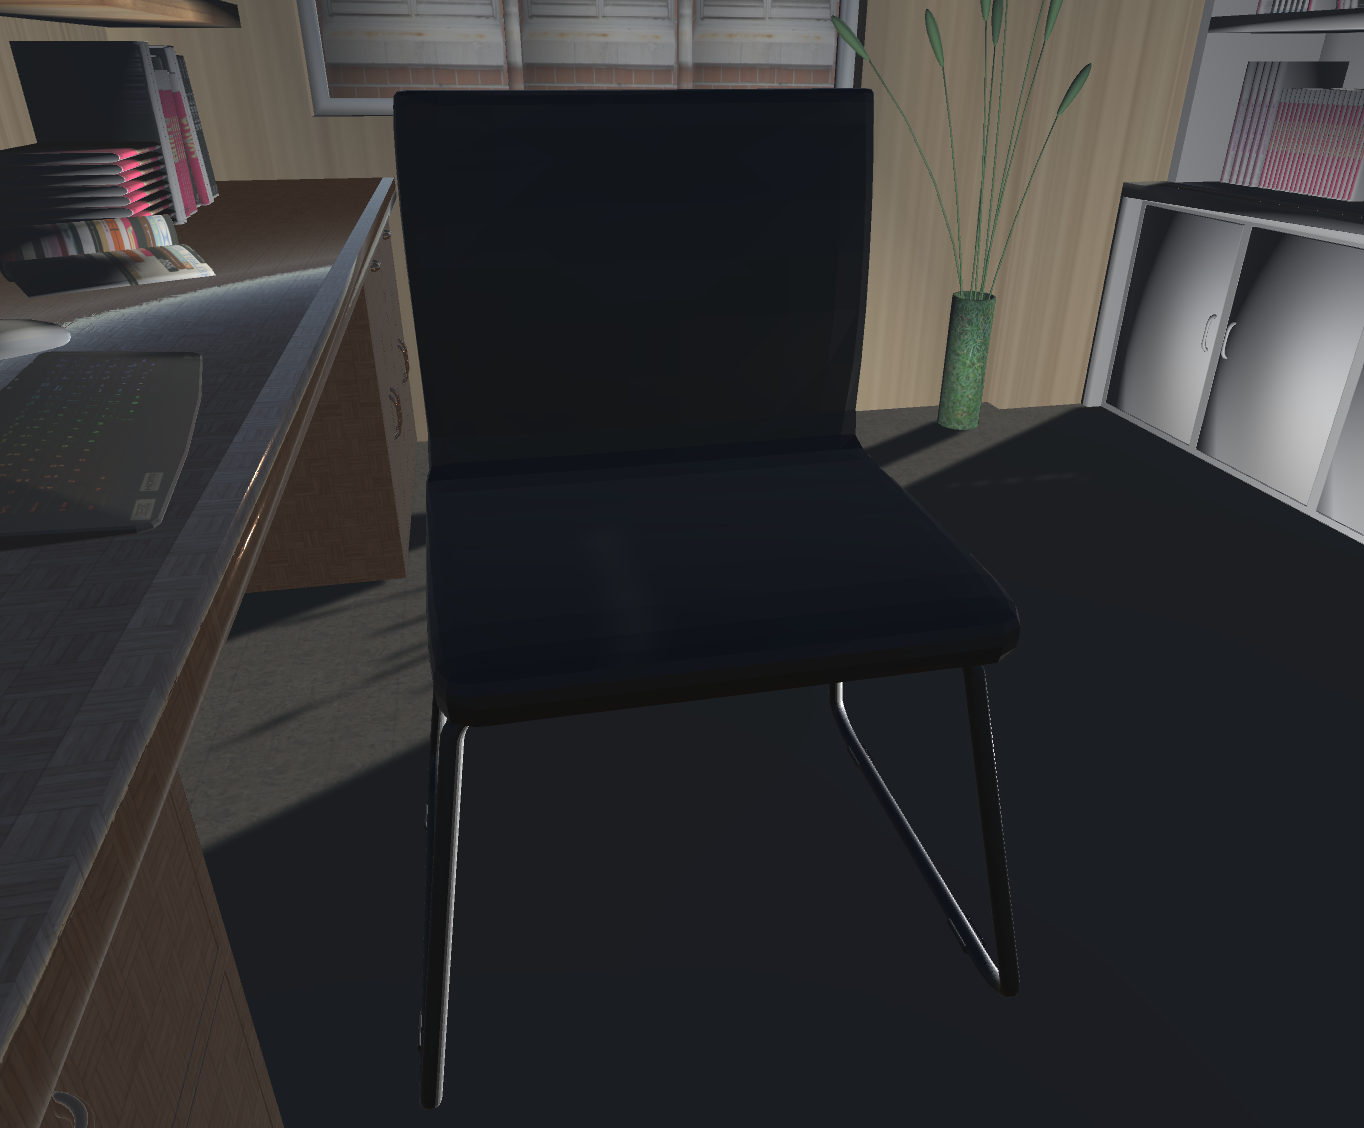
\includegraphics[width=.24\linewidth,valign=m]{/Users/apple/OVGU/Thesis/code/3dReconstruction/report/images/implementation/randomisation/lighting4}\\
    \vspace{0.1cm}
        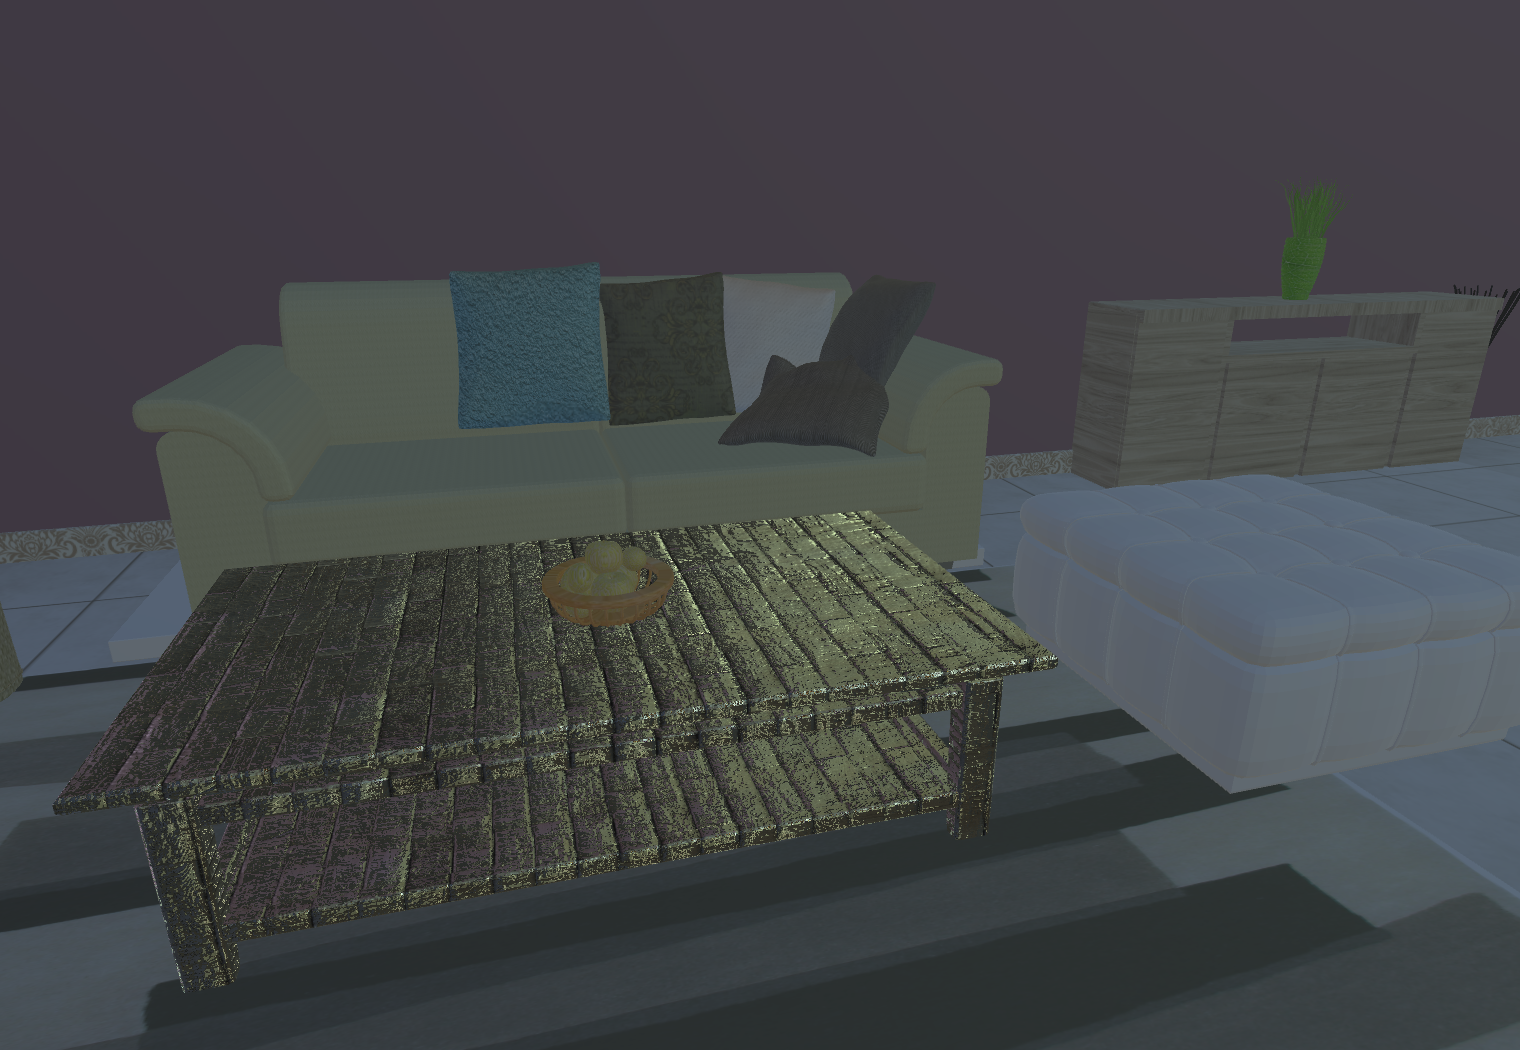
\includegraphics[width=.24\linewidth,valign=m]{/Users/apple/OVGU/Thesis/code/3dReconstruction/report/images/implementation/randomisation/lighting5}
        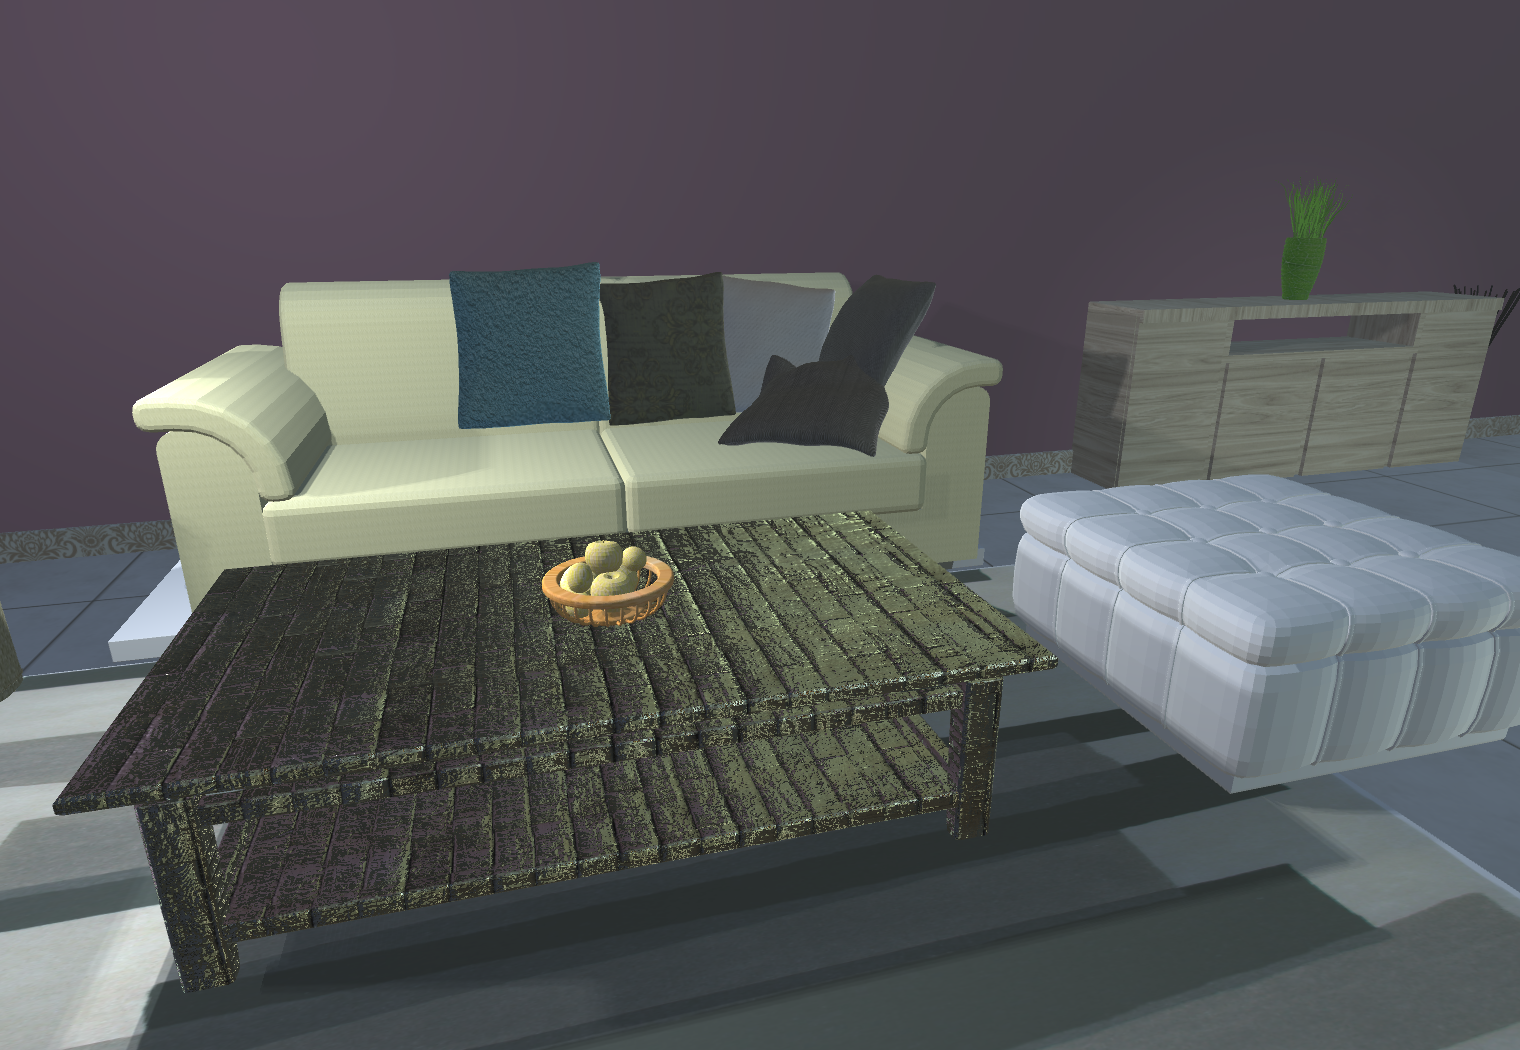
\includegraphics[width=.24\linewidth,valign=m]{/Users/apple/OVGU/Thesis/code/3dReconstruction/report/images/implementation/randomisation/lighting6}
        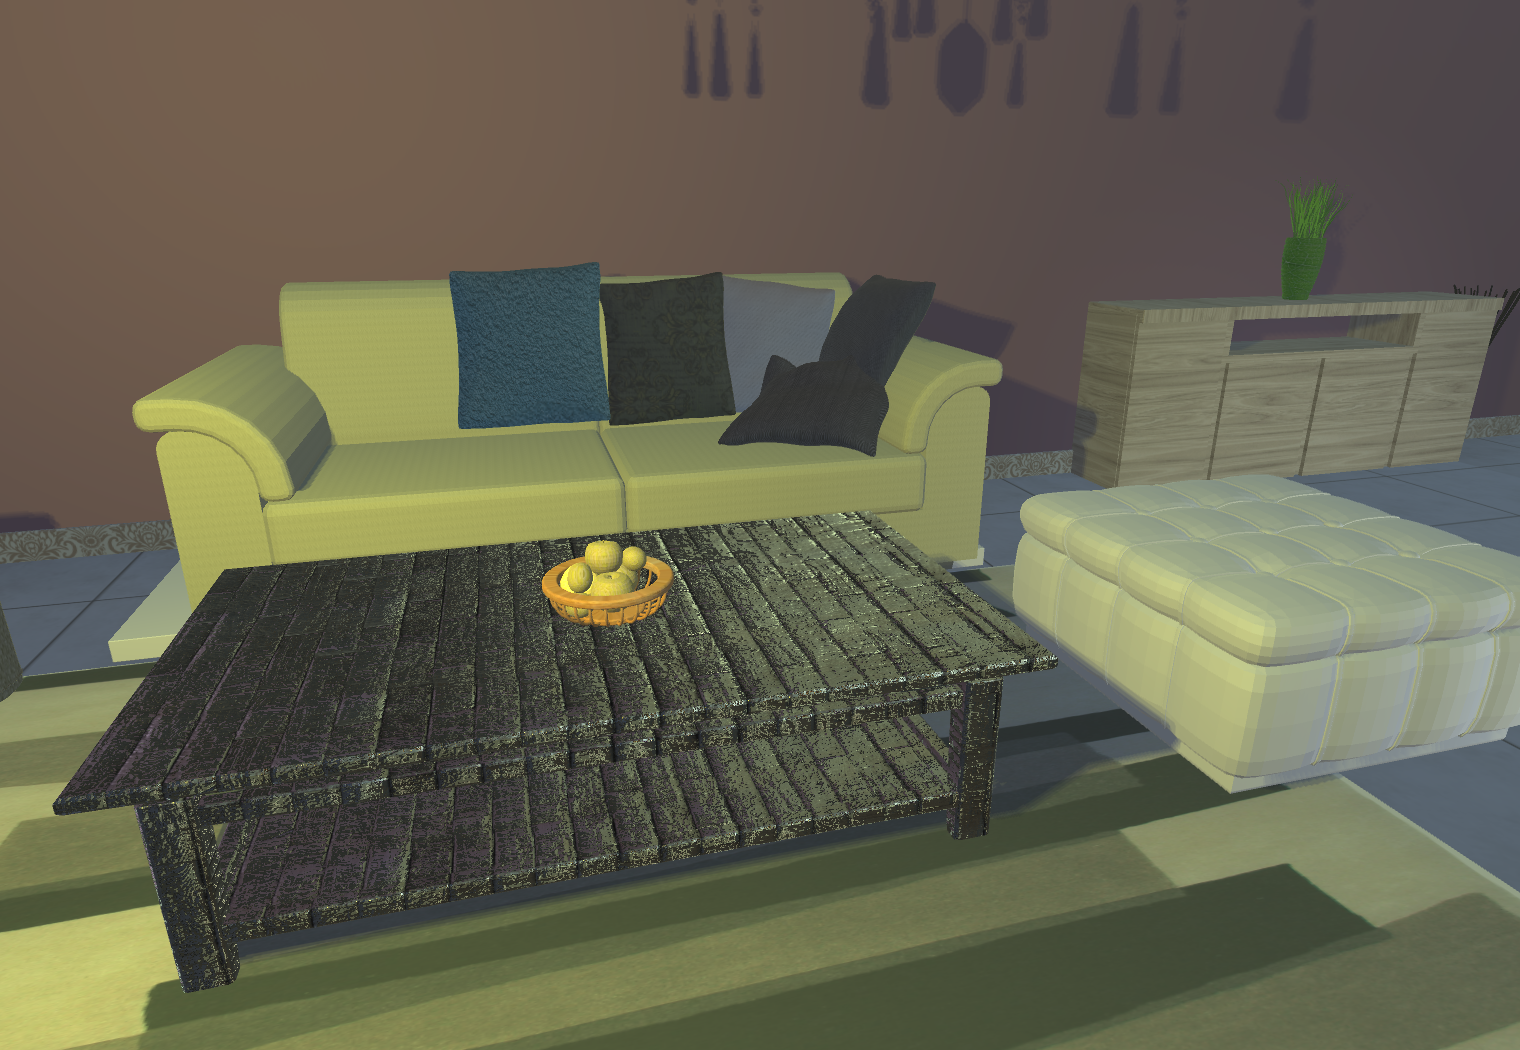
\includegraphics[width=.24\linewidth,valign=m]{/Users/apple/OVGU/Thesis/code/3dReconstruction/report/images/implementation/randomisation/lighting7}
        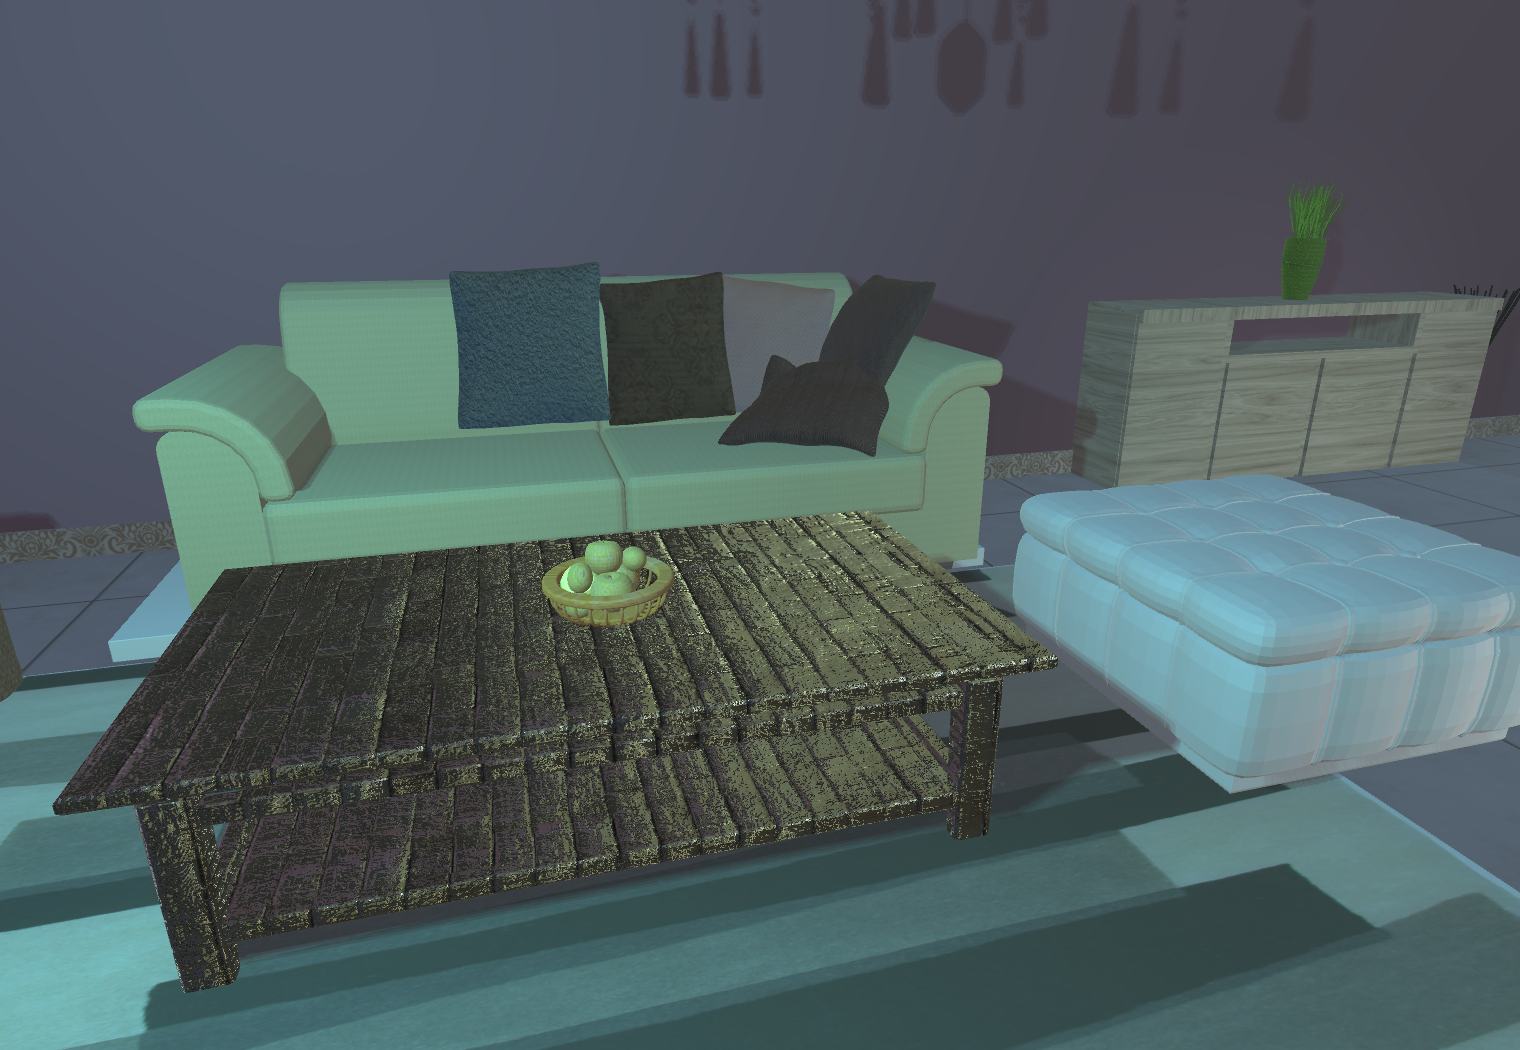
\includegraphics[width=.24\linewidth,valign=m]{/Users/apple/OVGU/Thesis/code/3dReconstruction/report/images/implementation/randomisation/lighting8}\\
    \caption{Sample images with different lighting and shadows conditions.First row is samples for light with different intensity and direction. Second row is differnt color for light.}
    \label{fig:Lighting and shadows}
\end{figure}

\subsection{Randomised Texture}

The objects in the scene are renamed to standard objects seen in day-to-day life.
The textures are grouped together to these names as folder names.
A total of 982 texture images, some of which are just JPG or PNG images, while there are few texutres from cctextures.com with more details like normals, displacement and roughness.
This makes the textures more realistic.
Distribution of textures used for randomisation of scenes is as shown in figure ~\ref{fig:Distribution of textures}, with categories of Pix3d having higher number of images.
Each scene is randomised for every snap taken of the target object.
Samples of texture randomisation of background in the scene with target object in the focus is as shown in figure ~\ref{fig:Texture Randomisation}.
Randomising outdoor environment is important in cases where we have open doors and windows.
Unity provides a wrapper for scenes called skyboxes.
This is something of a globe around the room under observation.
This gives us varying outdoor environment for the scene with sceneray at the horizon.
We randomize 10 skyboxes to achieve this. Samples of skybox is as shown in figure ~\ref{fig:skybox samples}.


\begin{figure}
    \centering
    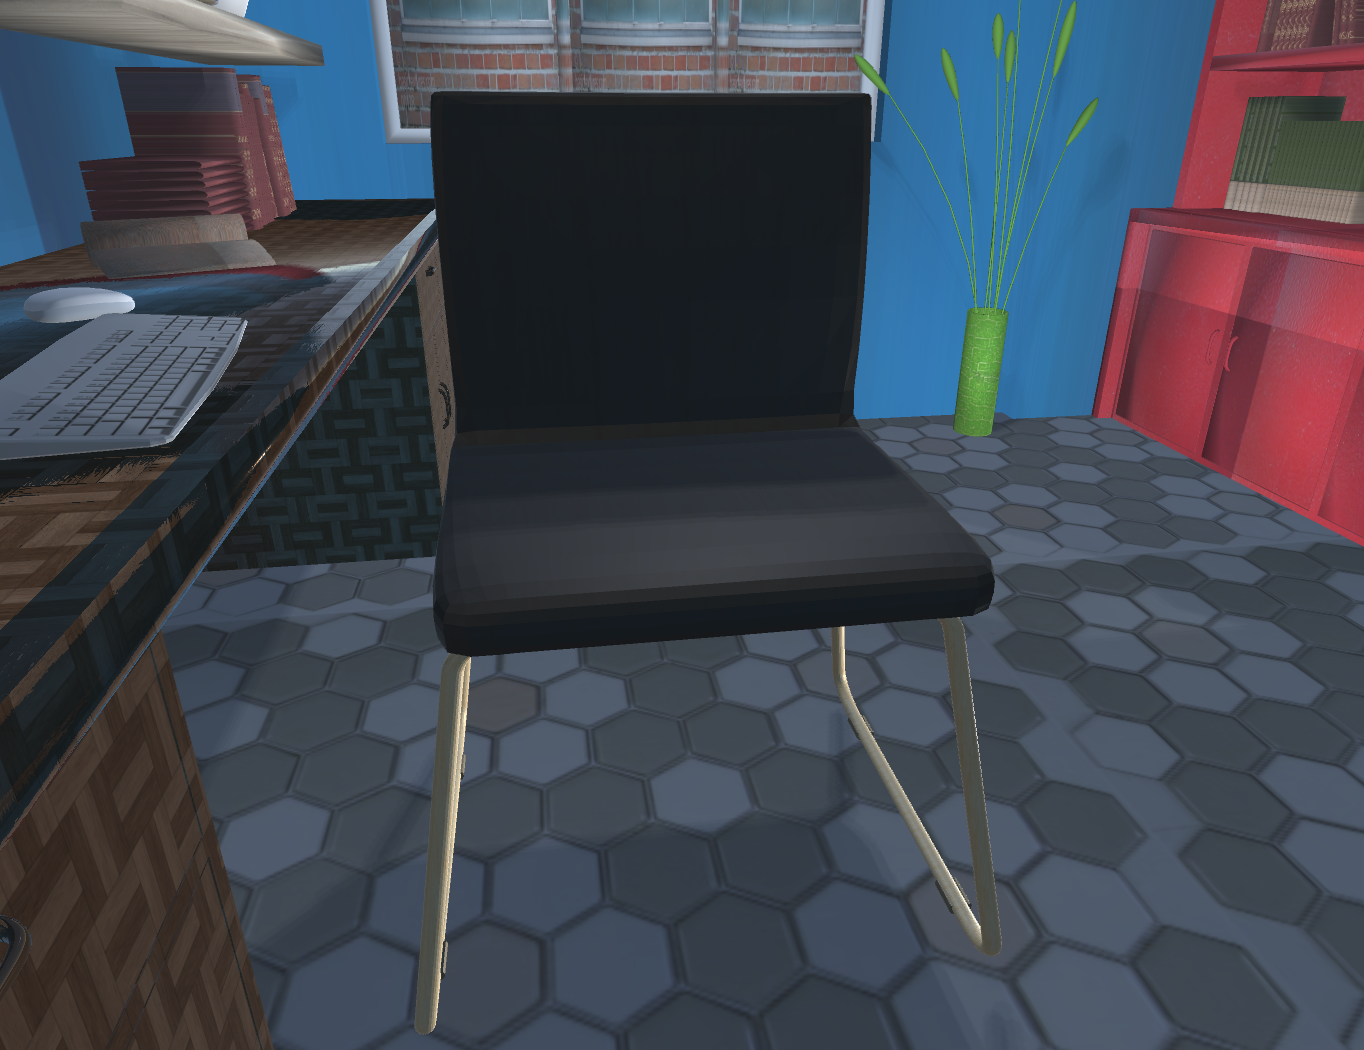
\includegraphics[width=.4\textwidth, height = .3\textwidth,valign=m]{/Users/apple/OVGU/Thesis/code/3dReconstruction/report/images/implementation/randomisation/background_texture1}
    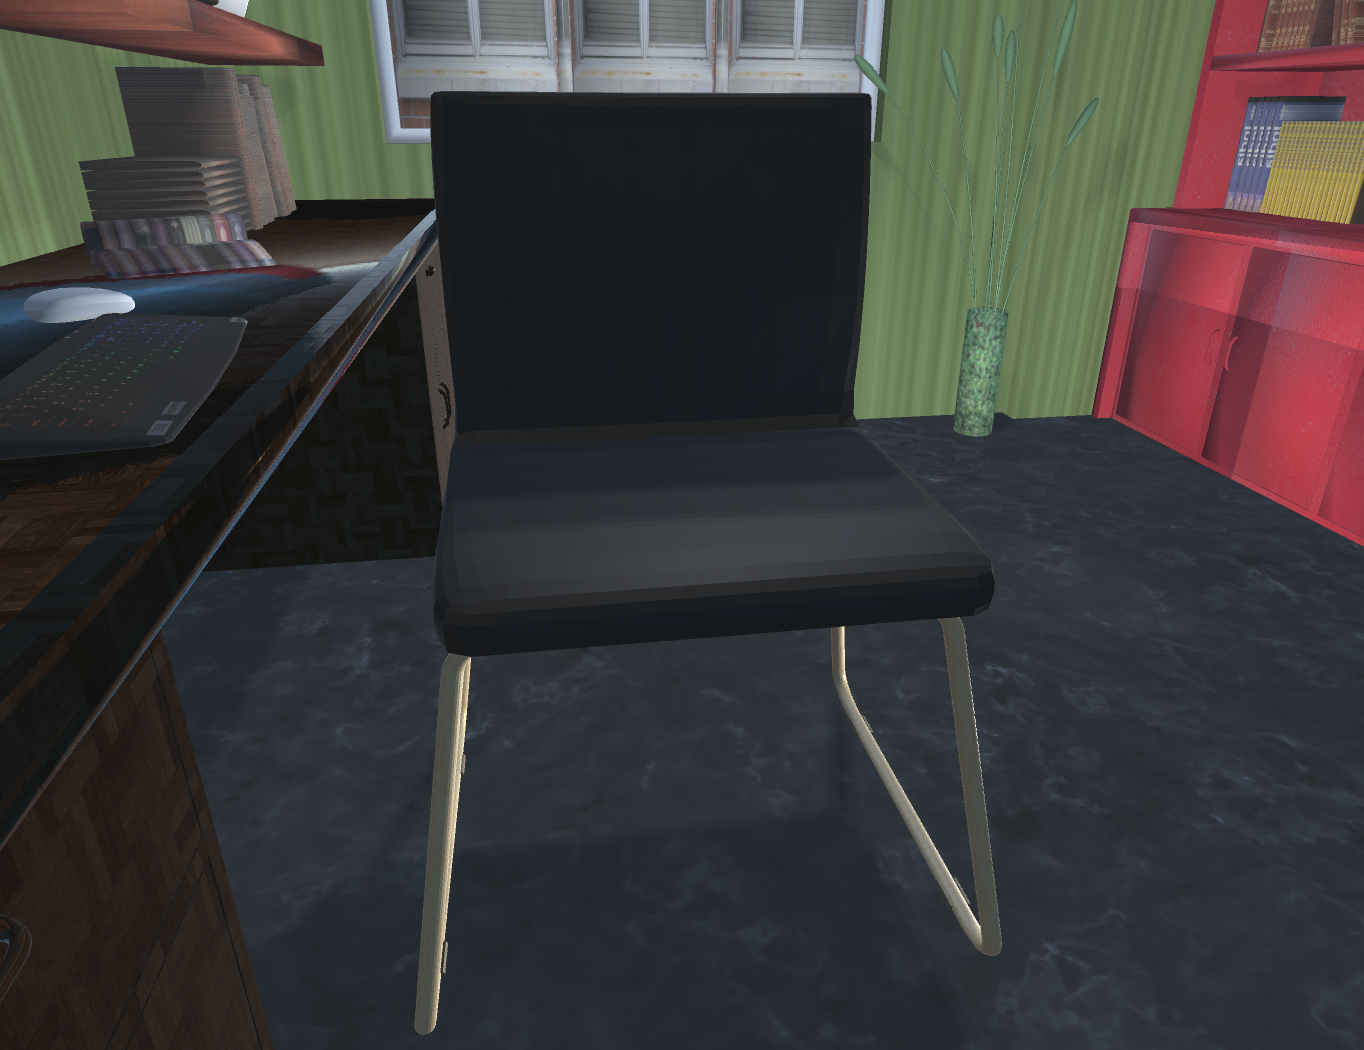
\includegraphics[width=.4\textwidth, height = .3\textwidth,valign=m]{/Users/apple/OVGU/Thesis/code/3dReconstruction/report/images/implementation/randomisation/background_texture2}\\
    \vspace{0.1cm}
    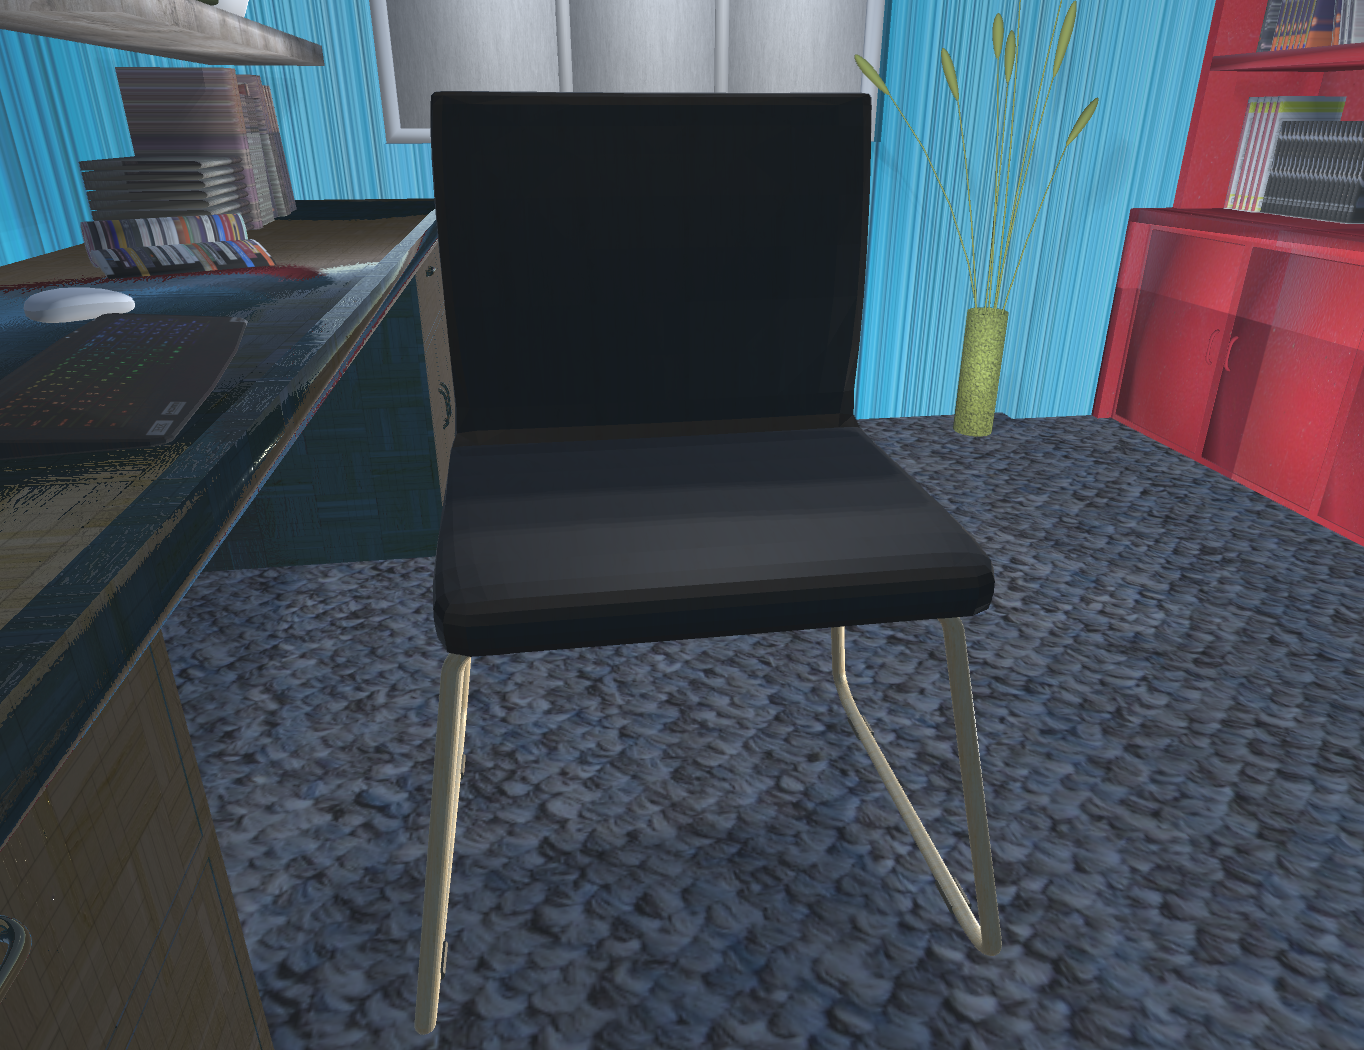
\includegraphics[width=.4\textwidth, height = .3\textwidth,valign=m]{/Users/apple/OVGU/Thesis/code/3dReconstruction/report/images/implementation/randomisation/background_texture3}
    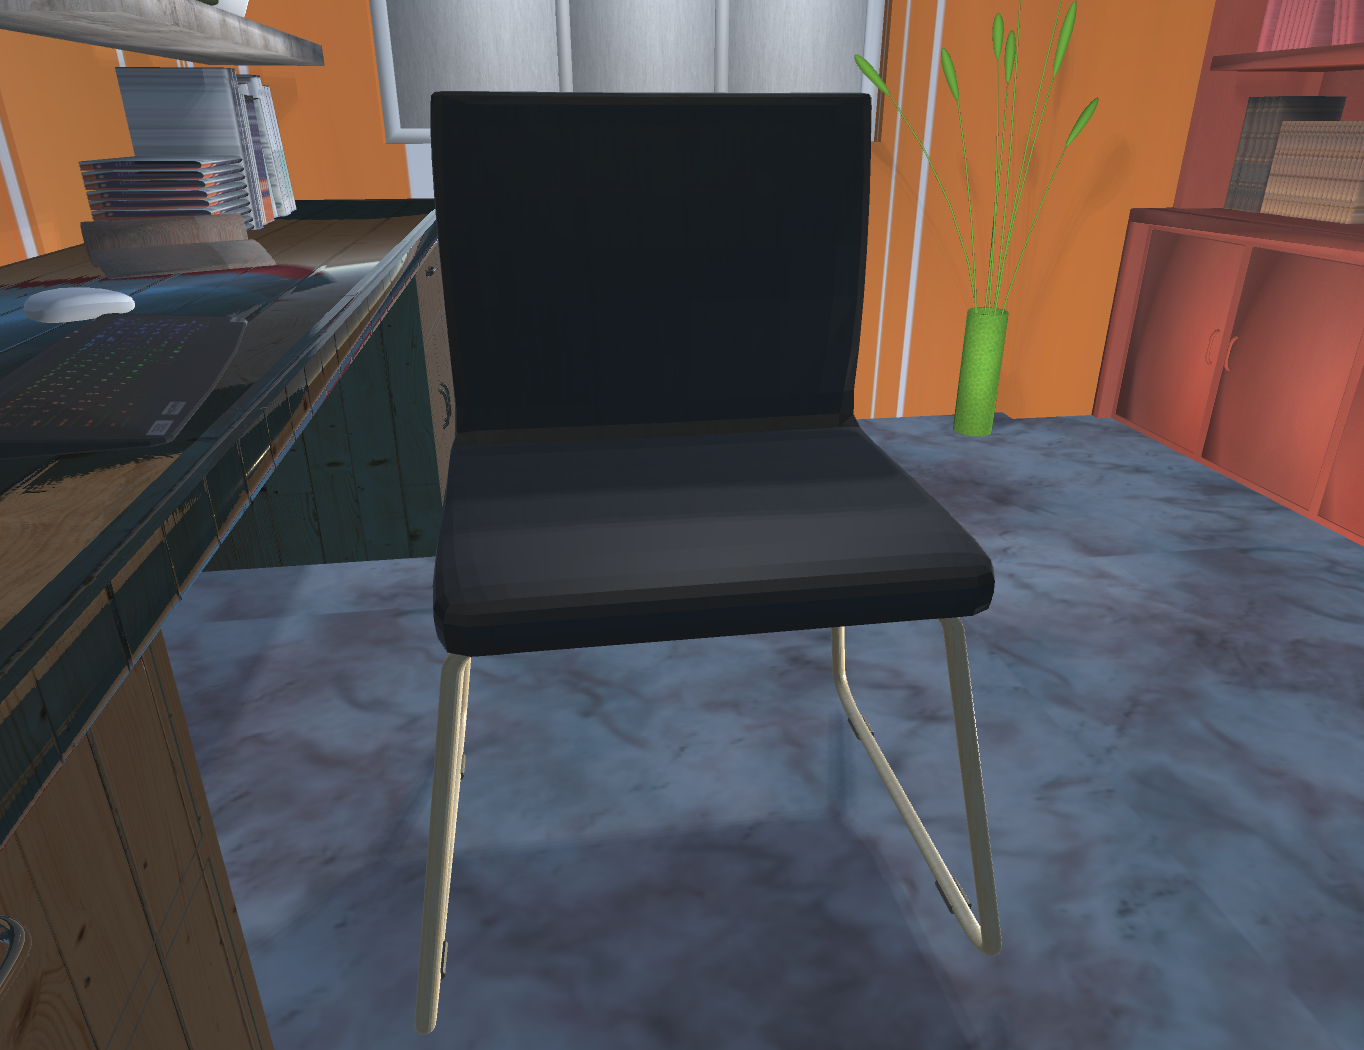
\includegraphics[width=.4\textwidth, height = .3\textwidth,valign=m]{/Users/apple/OVGU/Thesis/code/3dReconstruction/report/images/implementation/randomisation/background_texture4}\\
    \caption{Sample images with different textures for same scene.}
    \label{fig:Texture Randomisation}
\end{figure}

\begin{figure}
    \centering
    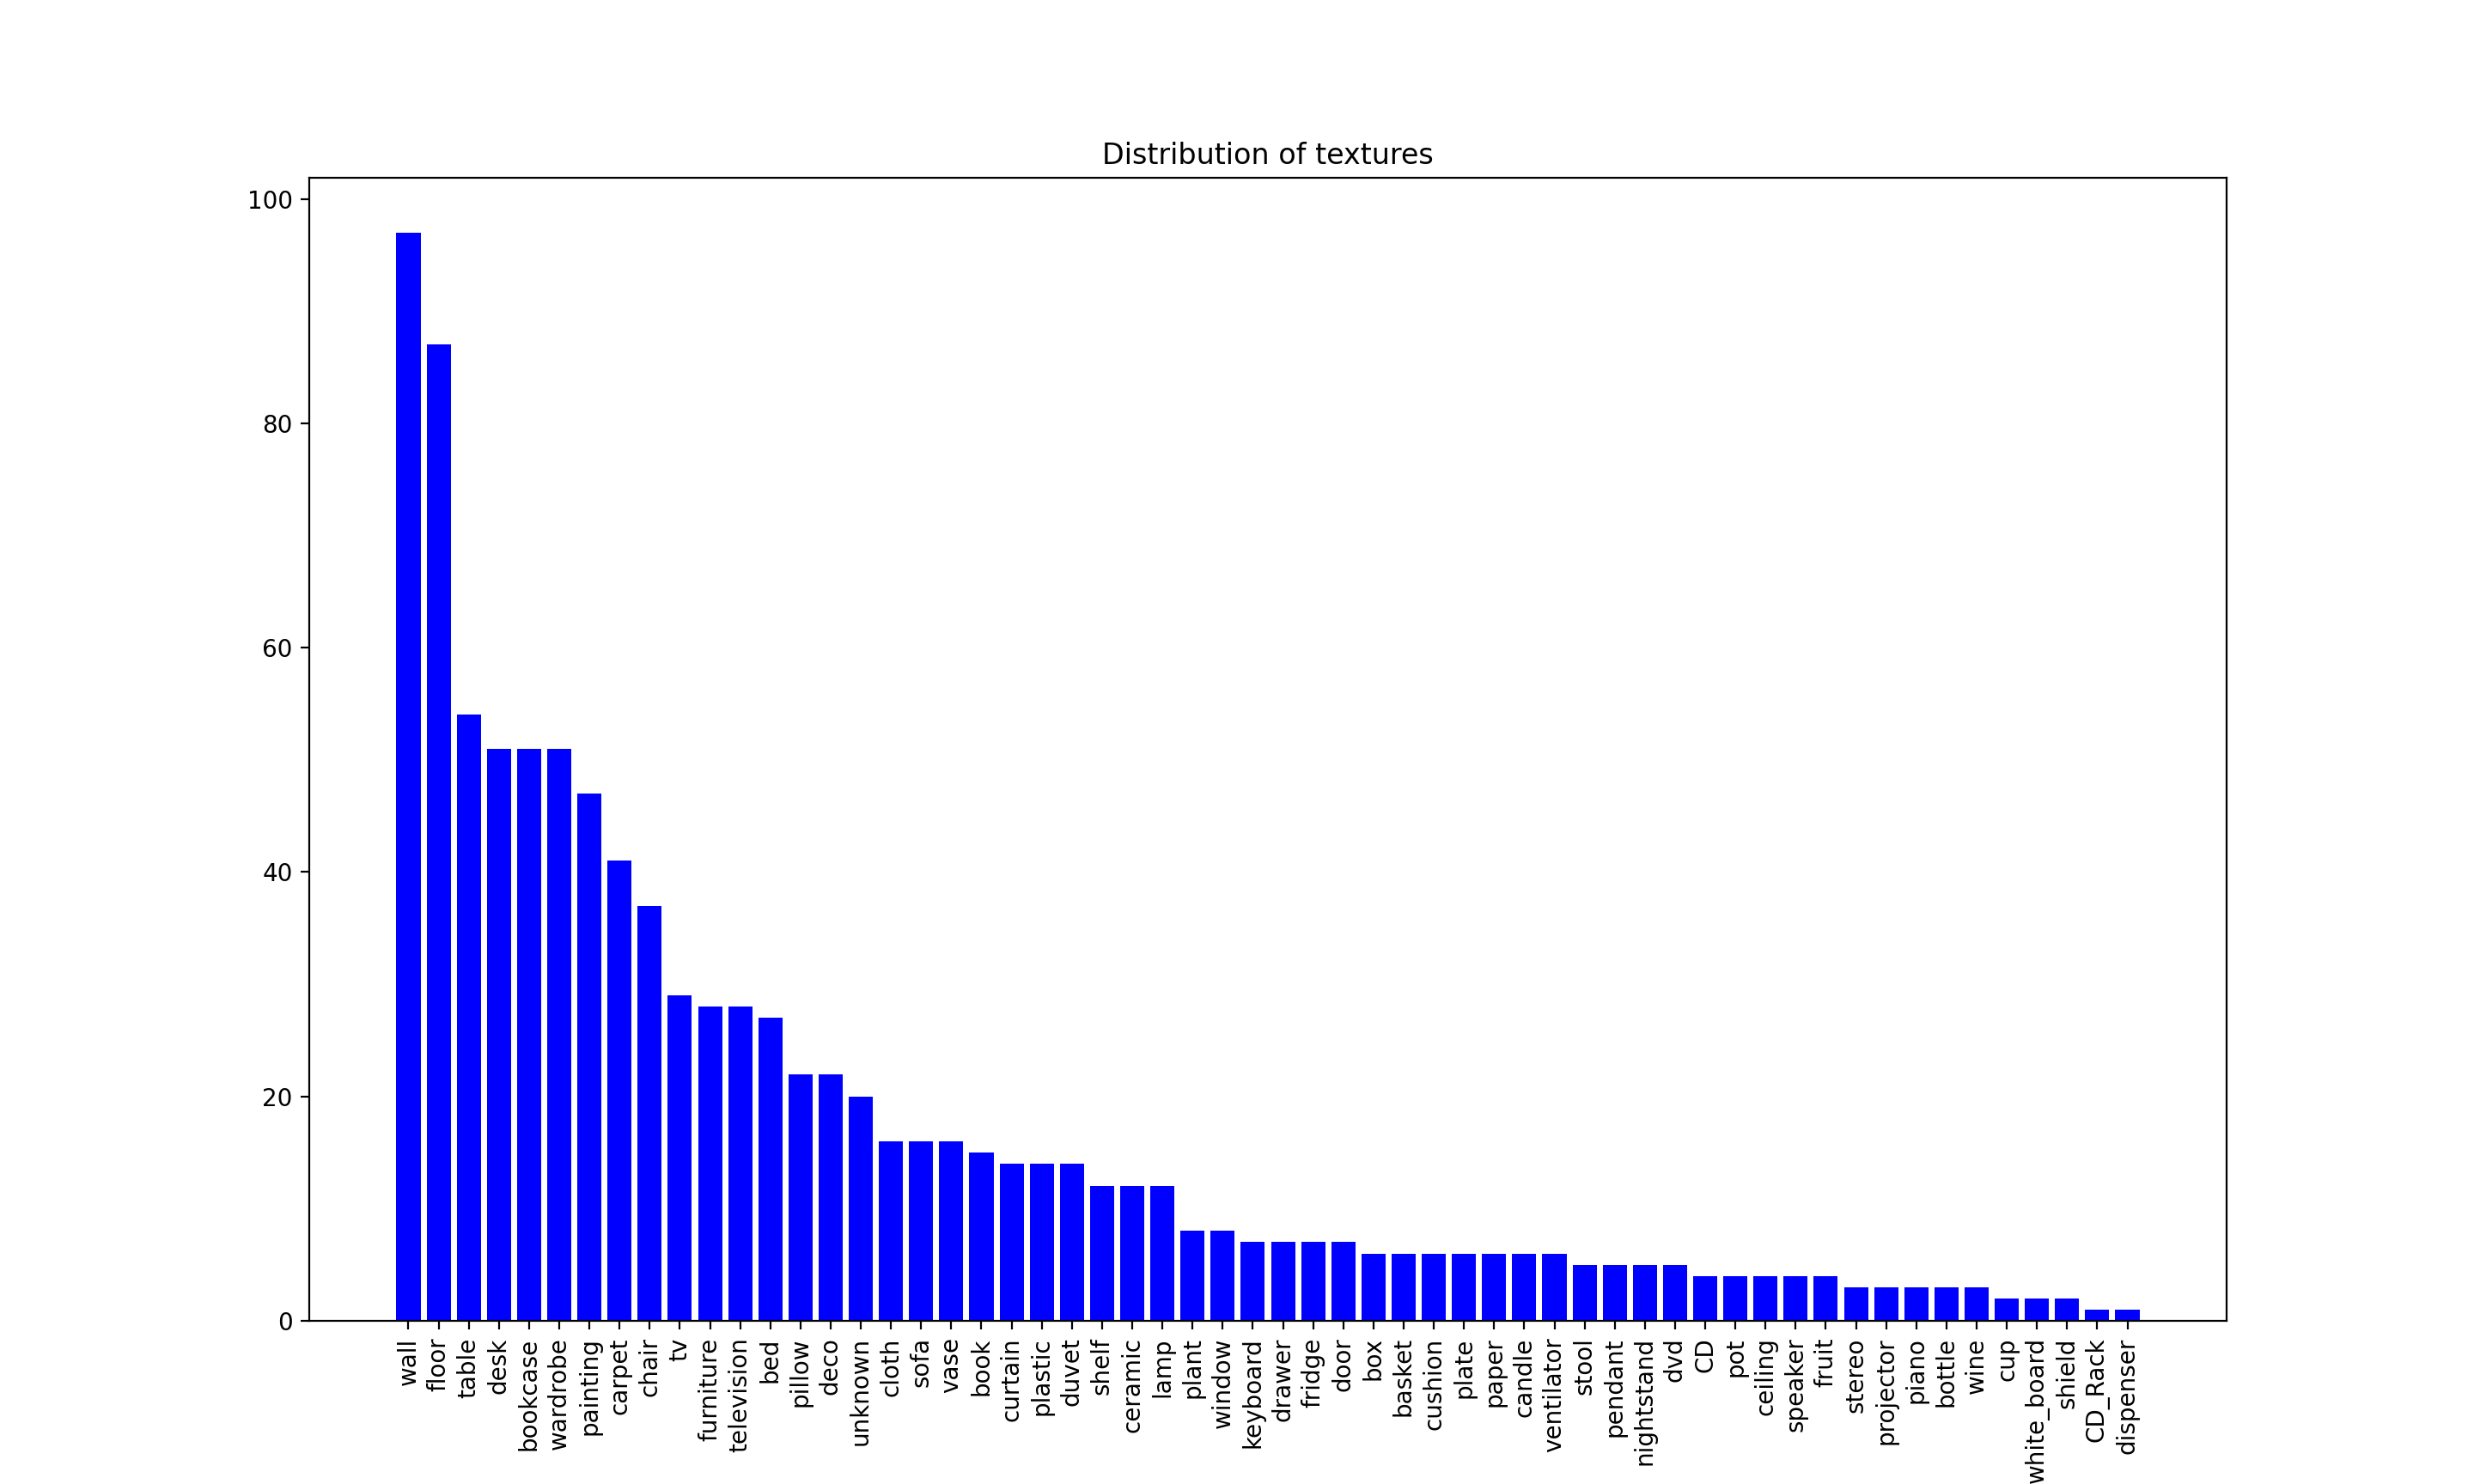
\includegraphics[width=\textwidth,valign=m]{/Users/apple/OVGU/Thesis/code/3dReconstruction/report/images/implementation/scenenet_scenes/distribution_of_textures}
    \caption{Distribution of textures used on scenes. The categories of pix3d(target furnitures) have higher number of images.}
    \label{fig:Distribution of textures}
\end{figure}

\begin{figure}
    \centering
        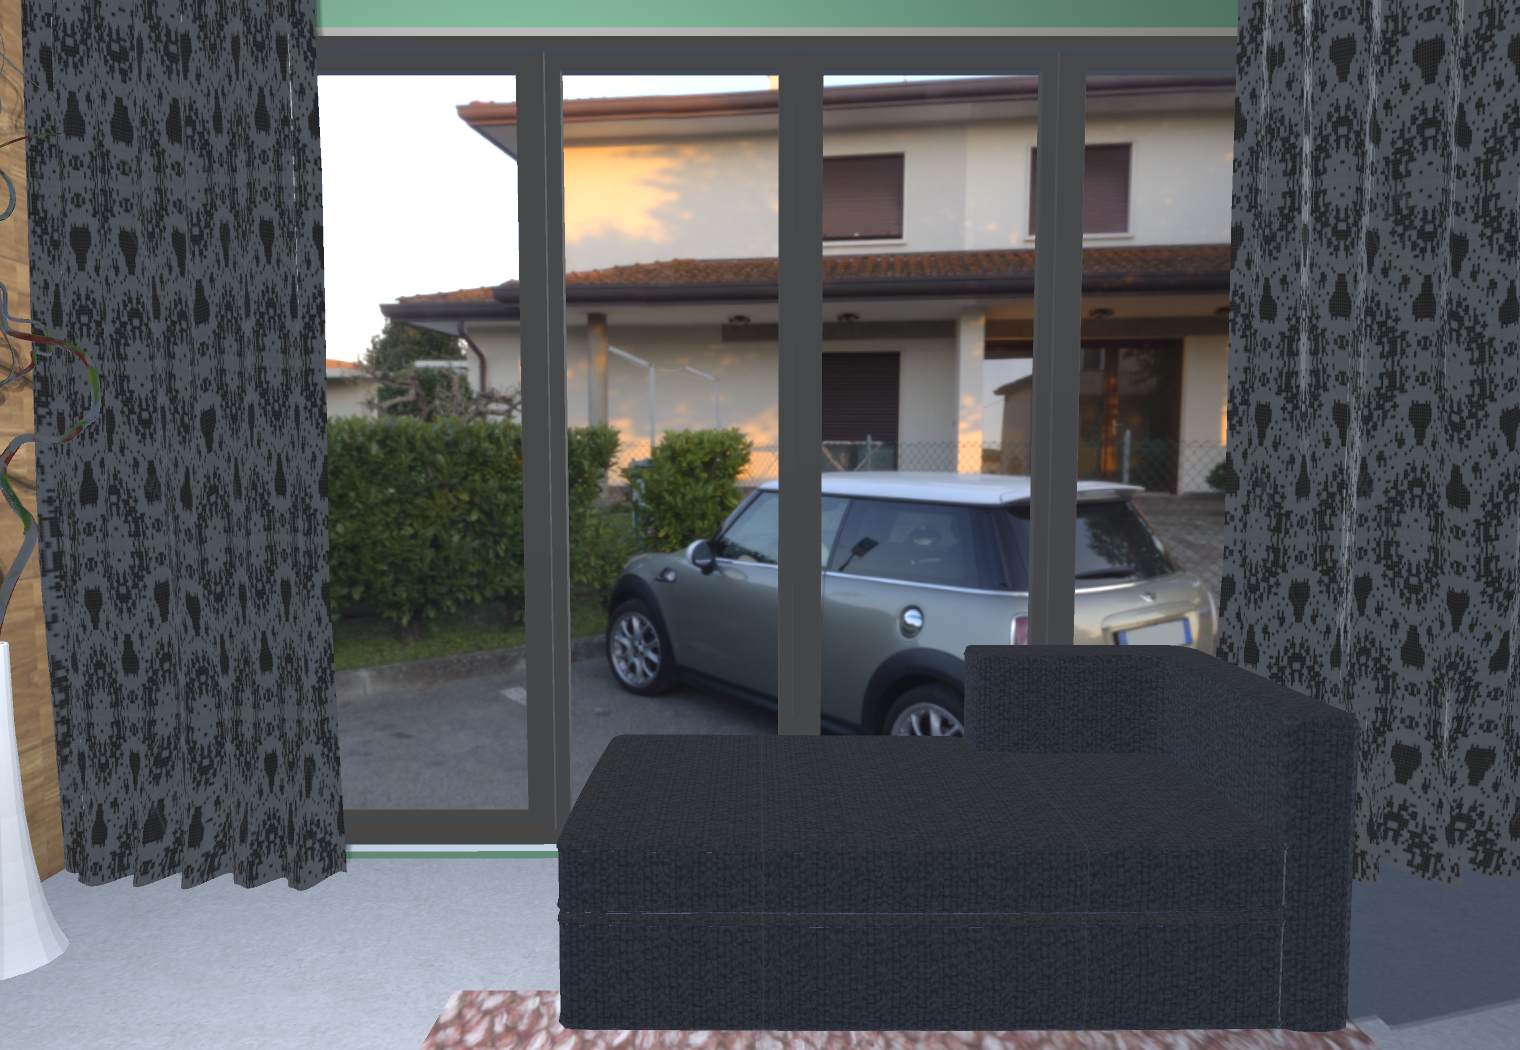
\includegraphics[width=.4\textwidth, height = .3\textwidth,valign=m]{/Users/apple/OVGU/Thesis/code/3dReconstruction/report/images/implementation/randomisation/skybox_1}
        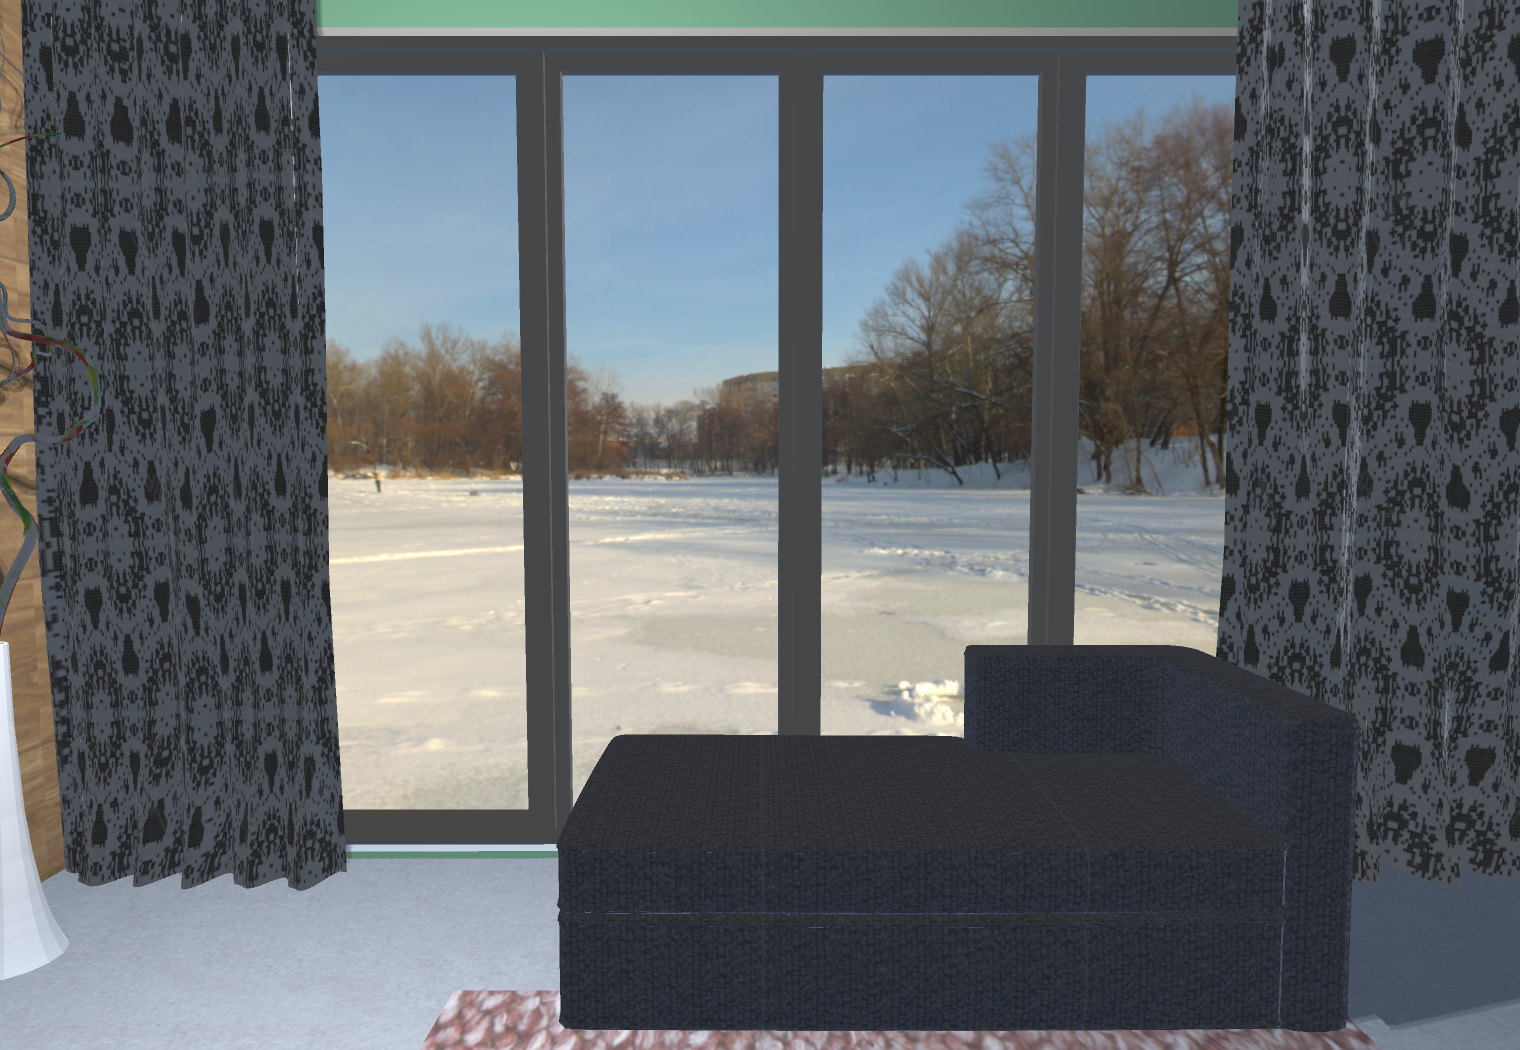
\includegraphics[width=.4\textwidth, height = .3\textwidth,valign=m]{/Users/apple/OVGU/Thesis/code/3dReconstruction/report/images/implementation/randomisation/skybox_2} \\
        \vspace{0.1cm}
        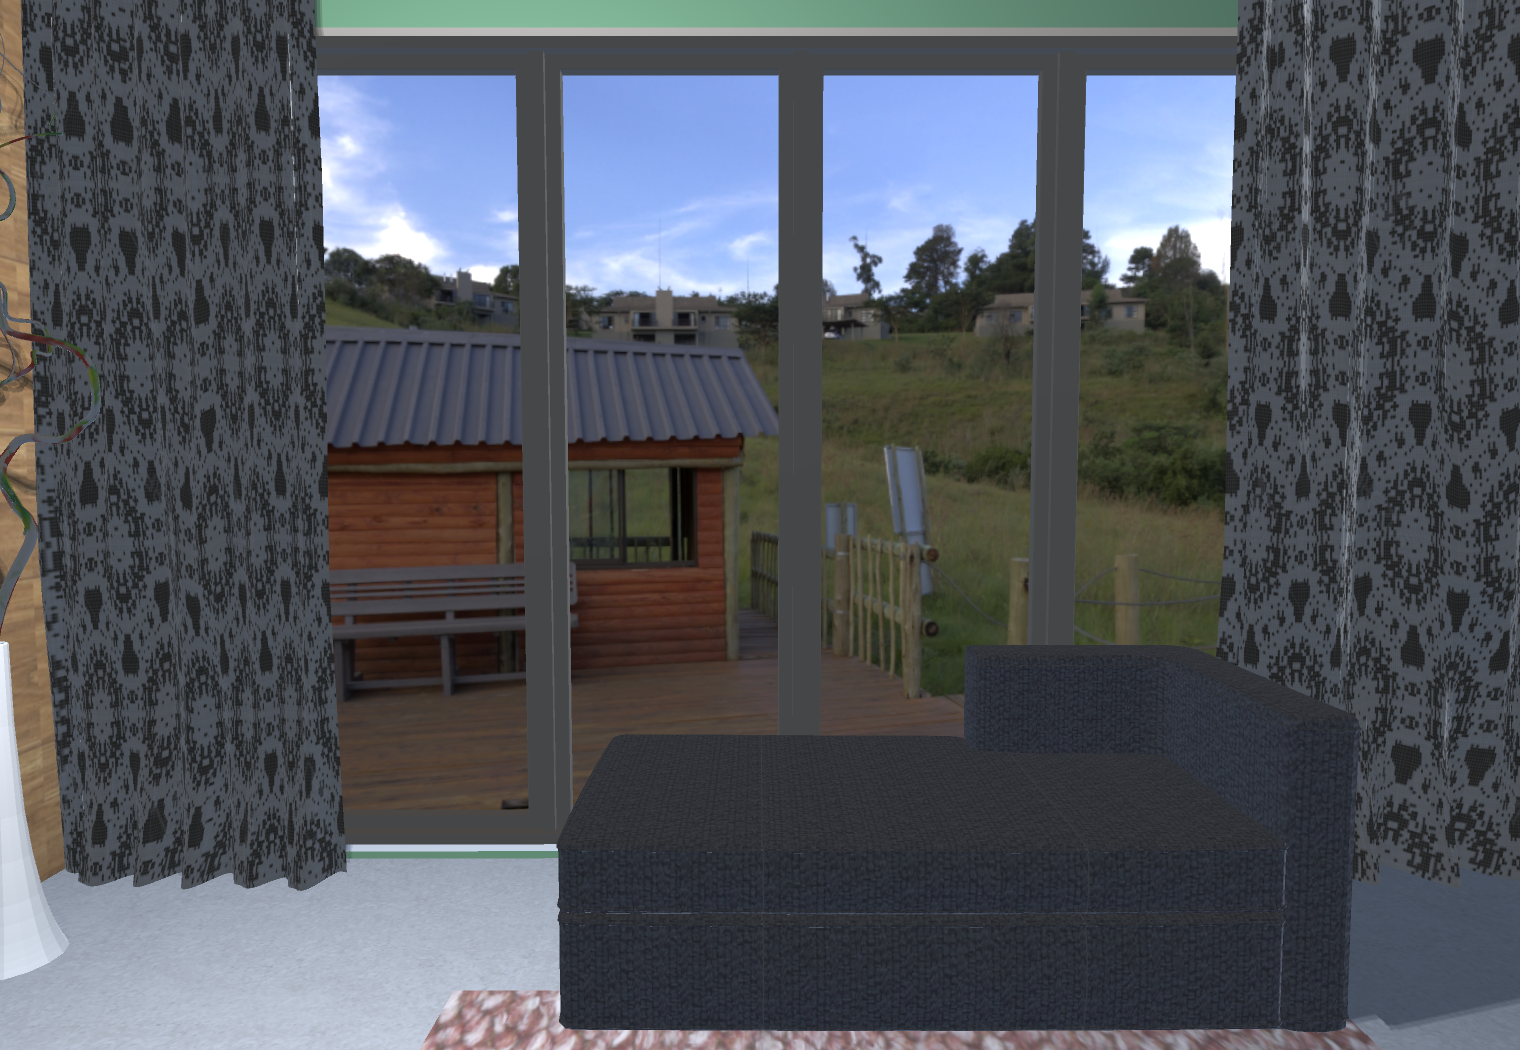
\includegraphics[width=.4\textwidth, height = .3\textwidth,valign=m]{/Users/apple/OVGU/Thesis/code/3dReconstruction/report/images/implementation/randomisation/skybox_3}
        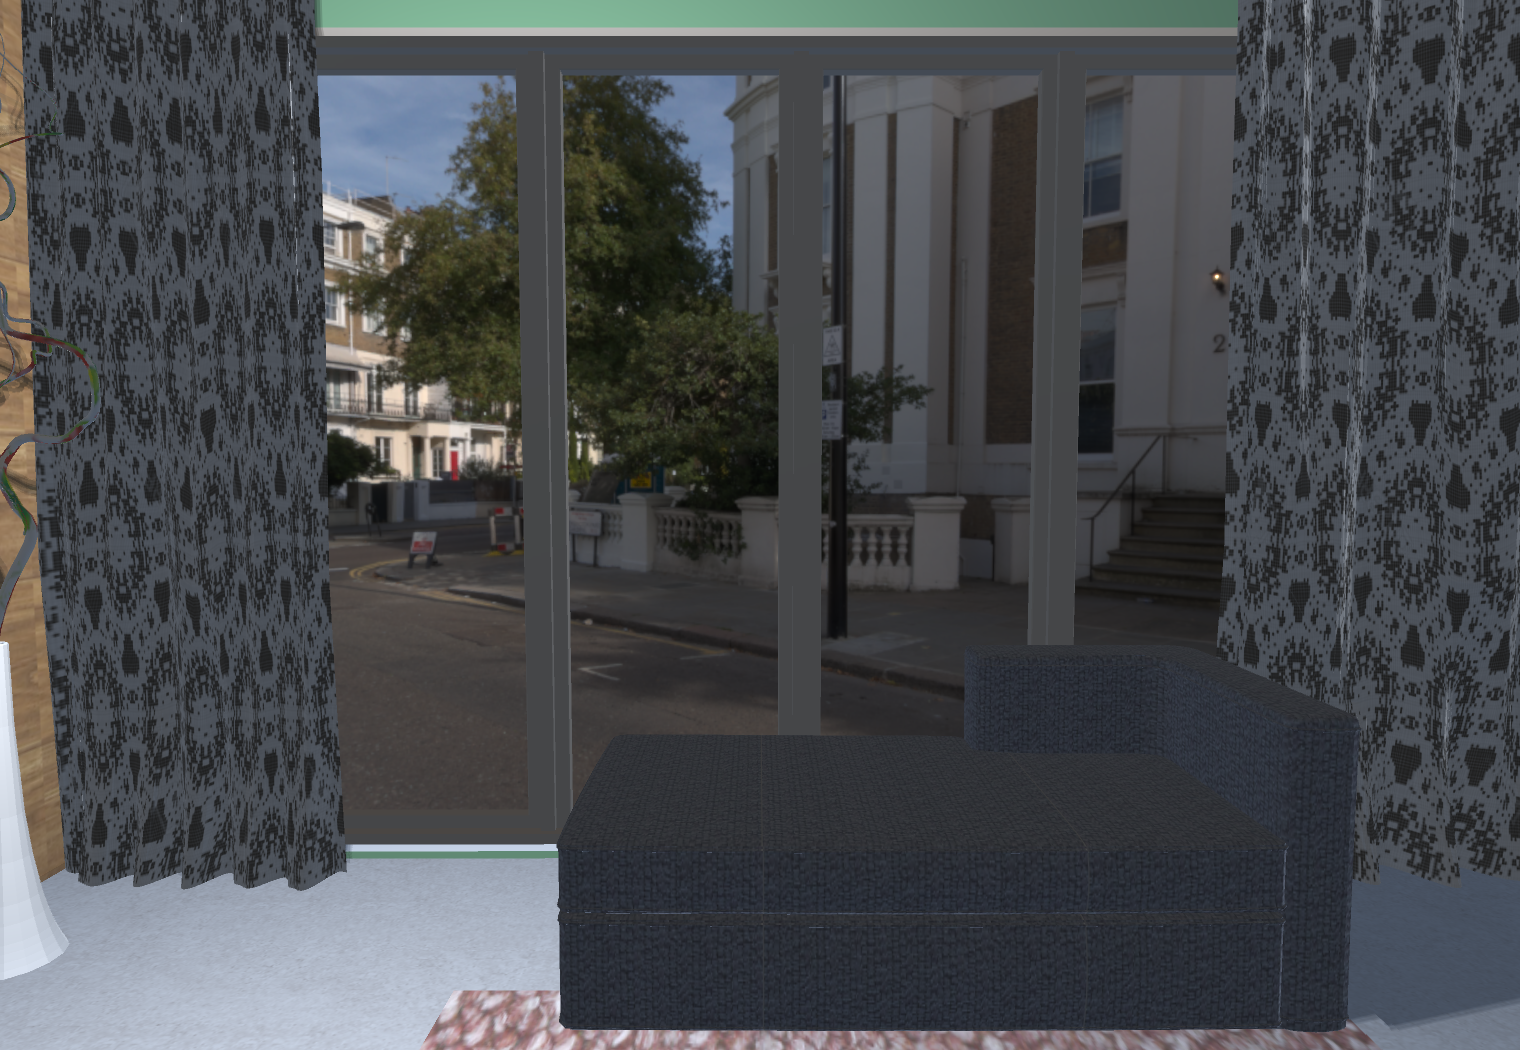
\includegraphics[width=.4\textwidth, height = .3\textwidth,valign=m]{/Users/apple/OVGU/Thesis/code/3dReconstruction/report/images/implementation/randomisation/skybox_4}\\
    \caption{Samples for different skyboxes which change the outdoor environment for the scenes. In the figure we see an open window with changing skybox.}
    \label{fig:skybox samples}
\end{figure}

\subsection{Replacing target Objects}

Once the room is setup using Scenenet ~\cite{McCormac:etal:ICCV2017} which contains objects from ShapeNet ~\cite{chang2015shapenet}, the objects are renamed such that it matches the classes for the Pix3D dataset.
Since a given scene can have more than one category under observation, a single model is chosen randomly out of all the present models.
The chosen model is replaced with a model in Pix3D of same category.
In case the replaced model is intersecting with any other models in the scene, we make it invisible.
Further, the camera checks if the centre of replaced model is in the frame.
If not, the camera viewpoint is changed untill it satisfies the condition.
After the snapshot is taken, the scene is reset to the original and next model is imported.
Samples for replacing a target object from original scene from Scenenet is shown in figure ~\ref{fig:replace model}

\begin{figure}
    \centering
        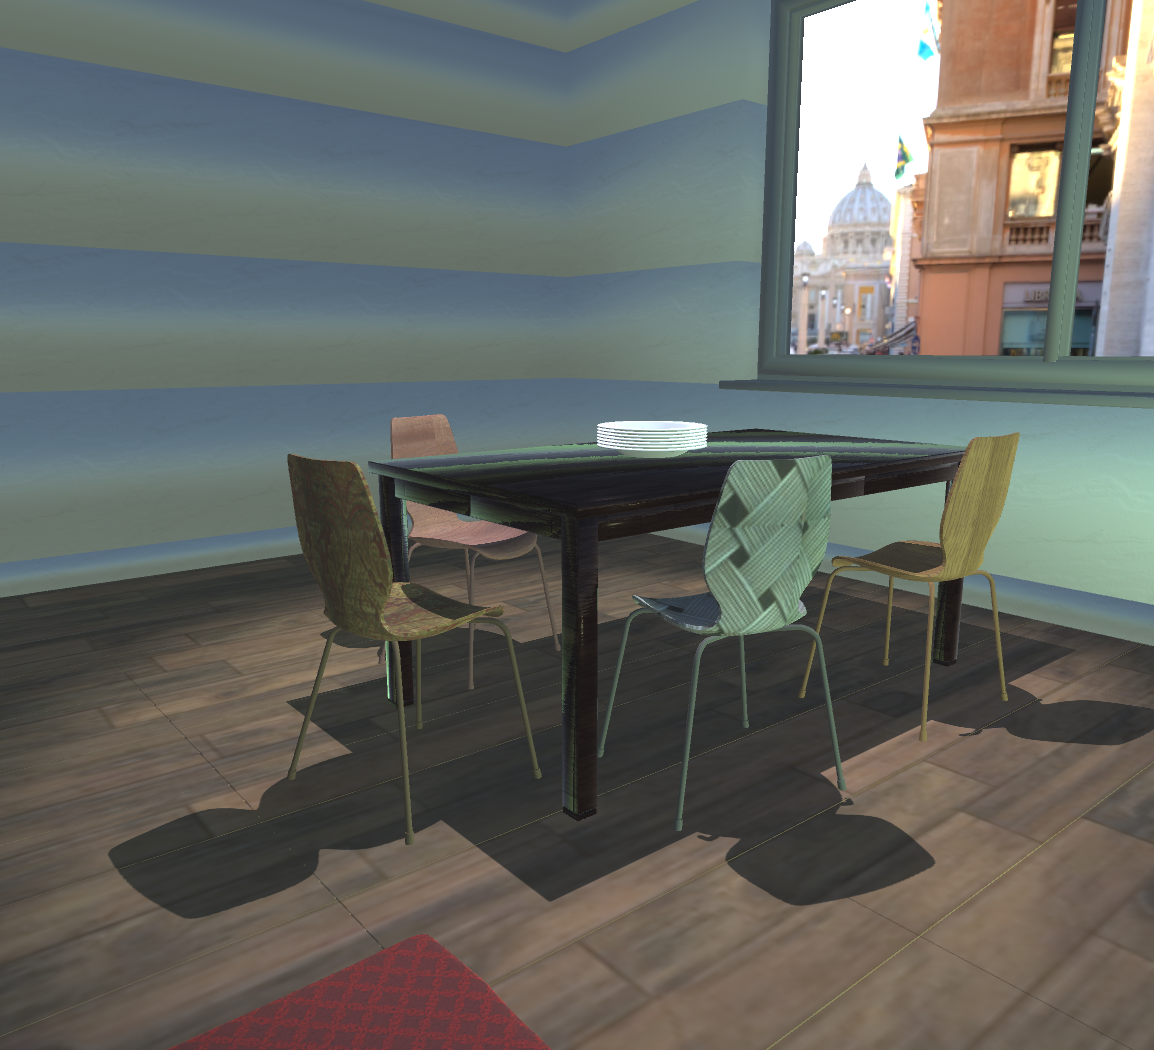
\includegraphics[width=.4\textwidth, height = .3\textwidth,valign=m]{/Users/apple/OVGU/Thesis/code/3dReconstruction/report/images/implementation/randomisation/replace_1-1}
        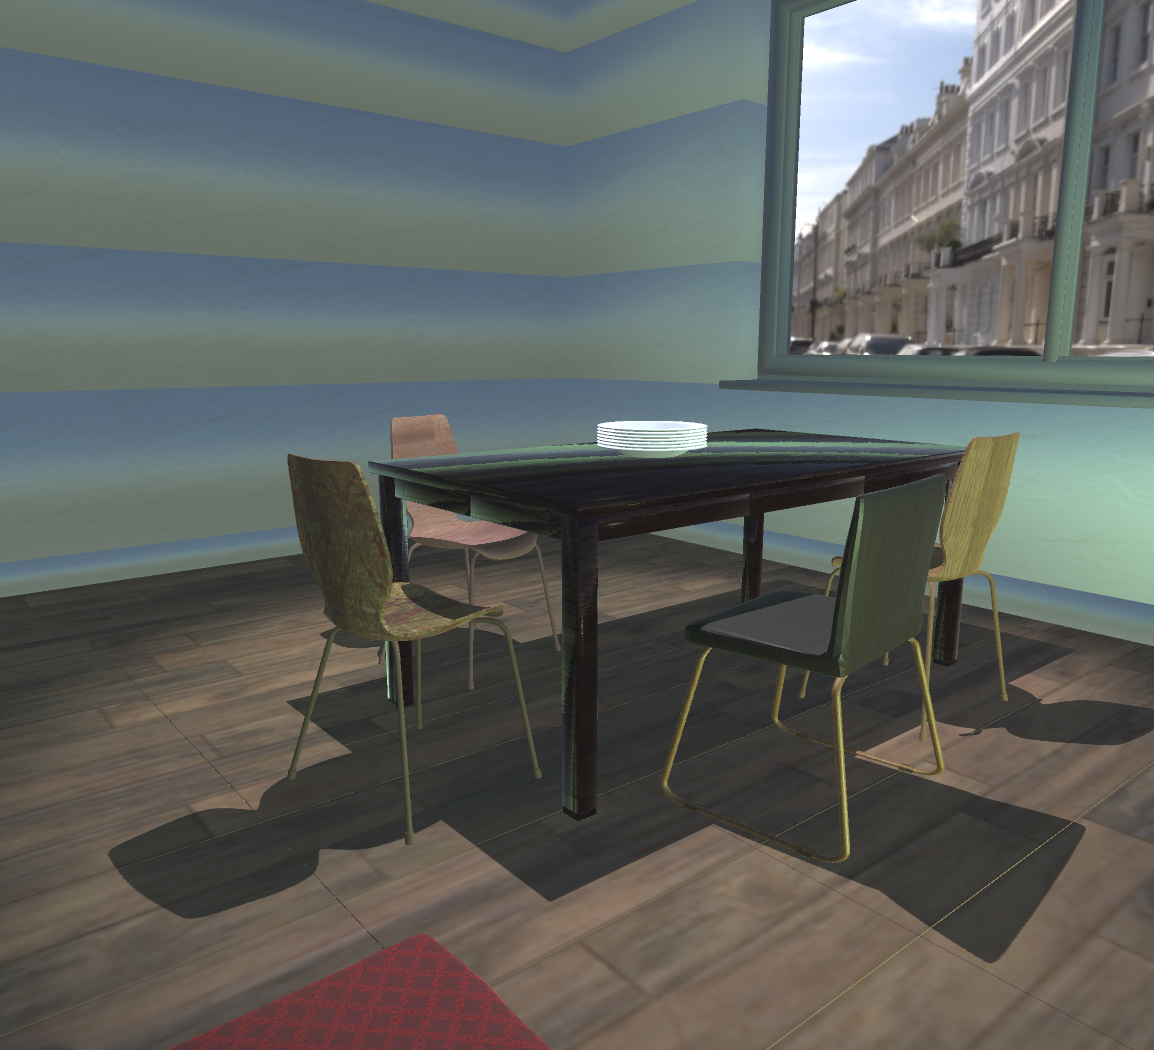
\includegraphics[width=.4\textwidth, height = .3\textwidth,valign=m]{/Users/apple/OVGU/Thesis/code/3dReconstruction/report/images/implementation/randomisation/replace_1-2} \\
        \vspace{0.1cm}
        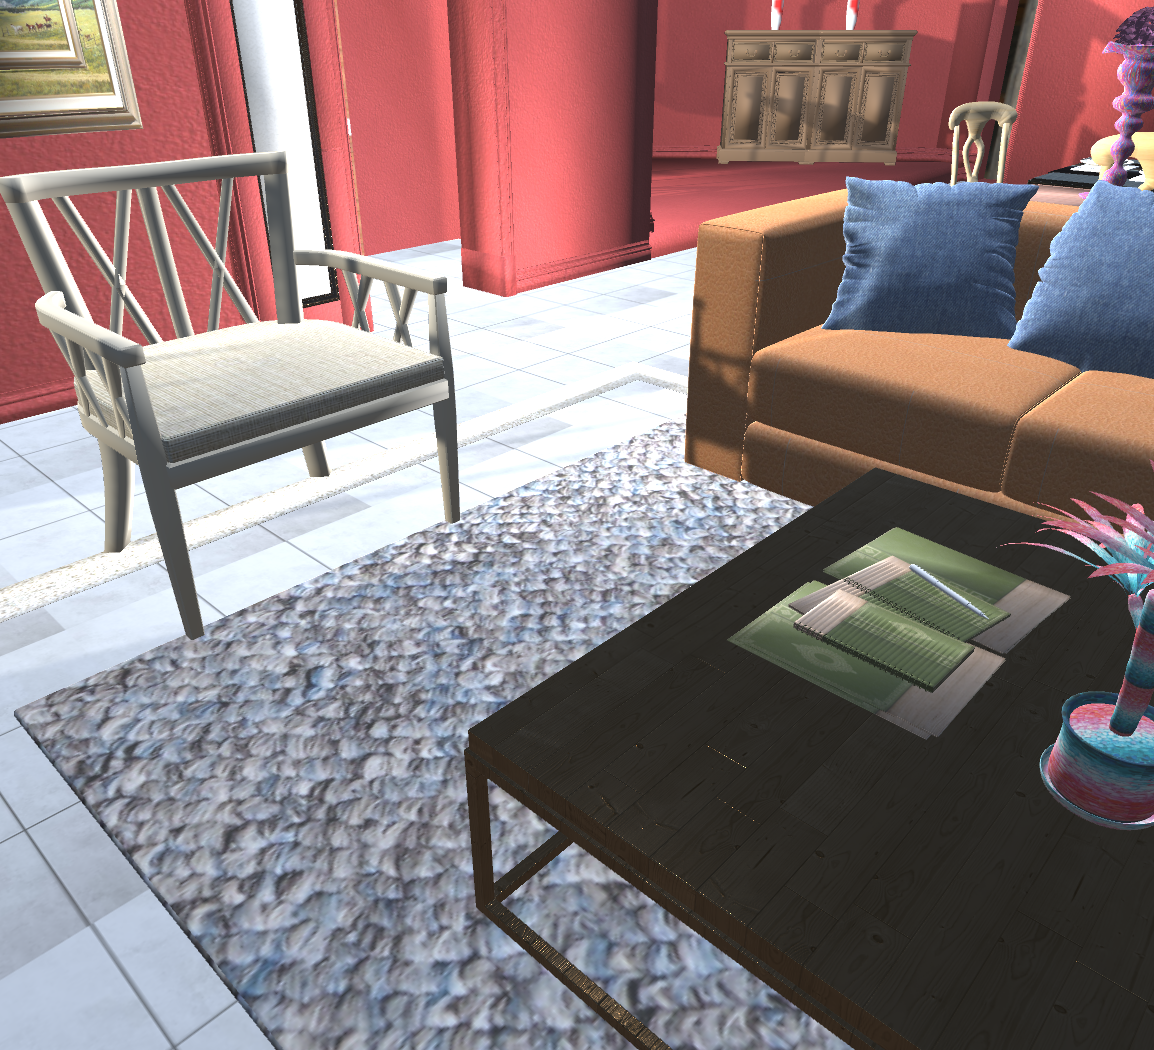
\includegraphics[width=.4\textwidth, height = .3\textwidth,valign=m]{/Users/apple/OVGU/Thesis/code/3dReconstruction/report/images/implementation/randomisation/replace_2-1}
        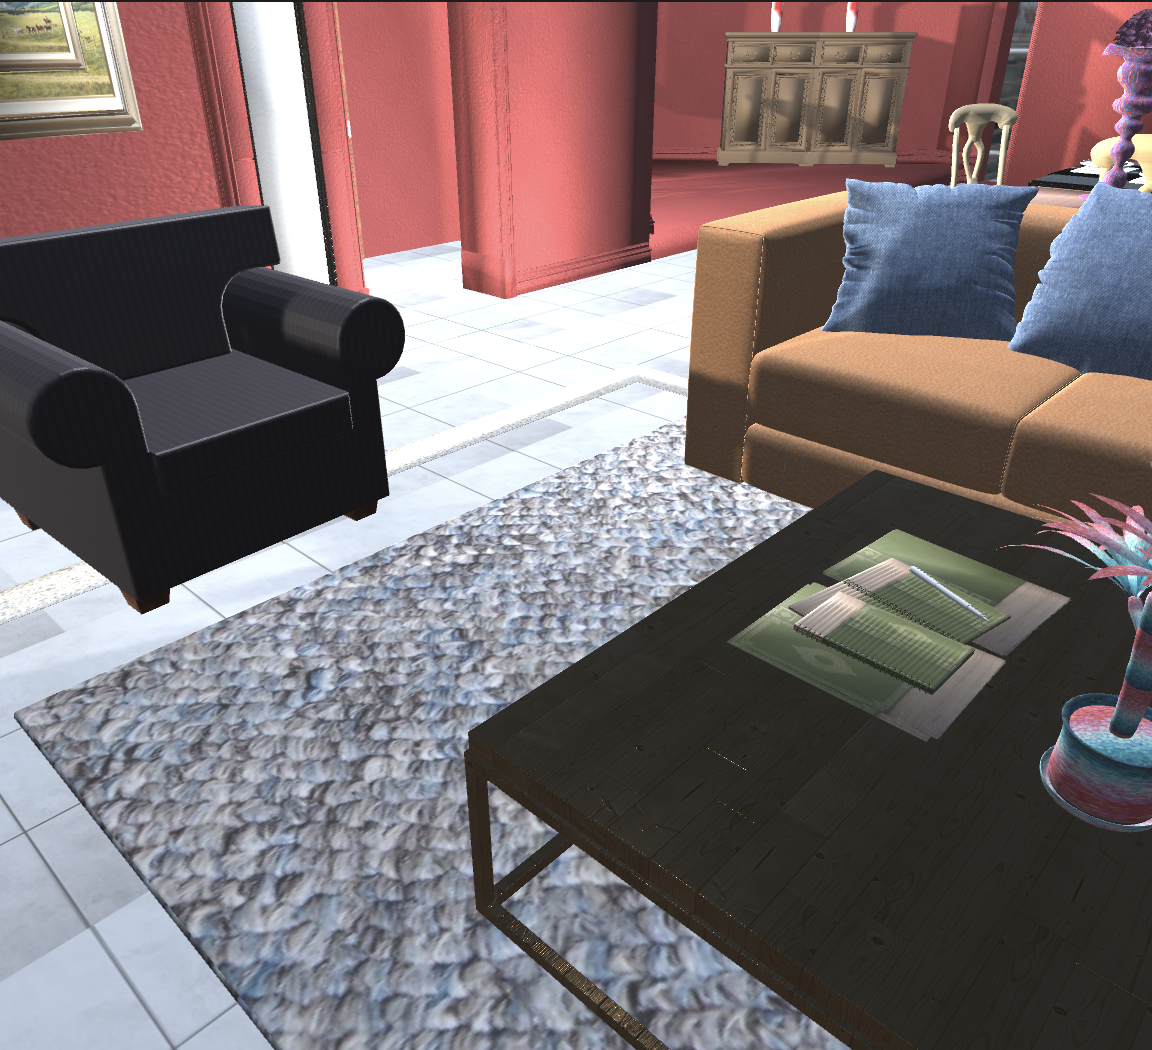
\includegraphics[width=.4\textwidth, height = .3\textwidth,valign=m]{/Users/apple/OVGU/Thesis/code/3dReconstruction/report/images/implementation/randomisation/replace_2-2}\\
    \caption{Samples for object replacement. The Left column shows a scene from SceneNet, while the right column shows an object being replaced in original scene.}
    \label{fig:replace model}
\end{figure}

\subsection{Snapshots with ML-ImageSynthesis}

ML-ImageSynthesis ~\cite{imagesynthesis} is a library provided by Unity to support synthetic dataset creation.
It supports the following G-buffers Image segmentation, Object categorization, Optical flow, Depth, Normals, etc.
G-buffers is basically a collective term to represent light-properties which are agregated to give the final rendering.
In image segmentation each object is assigned unique color.
In object categorization each category of the objects is assigned a single color.
For optical flow each pixel is colored depending on Unity's per-pixel Motion Vectors with respect to the camera.
Depth is as the word suggests the distance of each pixel from the camera encoded in 8-bit channels of the PNG image.
Normals are color encoding based on the orientation of object with respect to the camera.
For the snapshot, each of these properties is assigned a hidden camera and have each one overrides rendering scene with custom shaders to generate corresponding output.
These camera outputs can be seen in editor mode by changing the display window.
Samples of G-buffer collected for dataset are as shown in figure \ref{fig:G-buffers samples}.

\begin{figure}
    \centering
        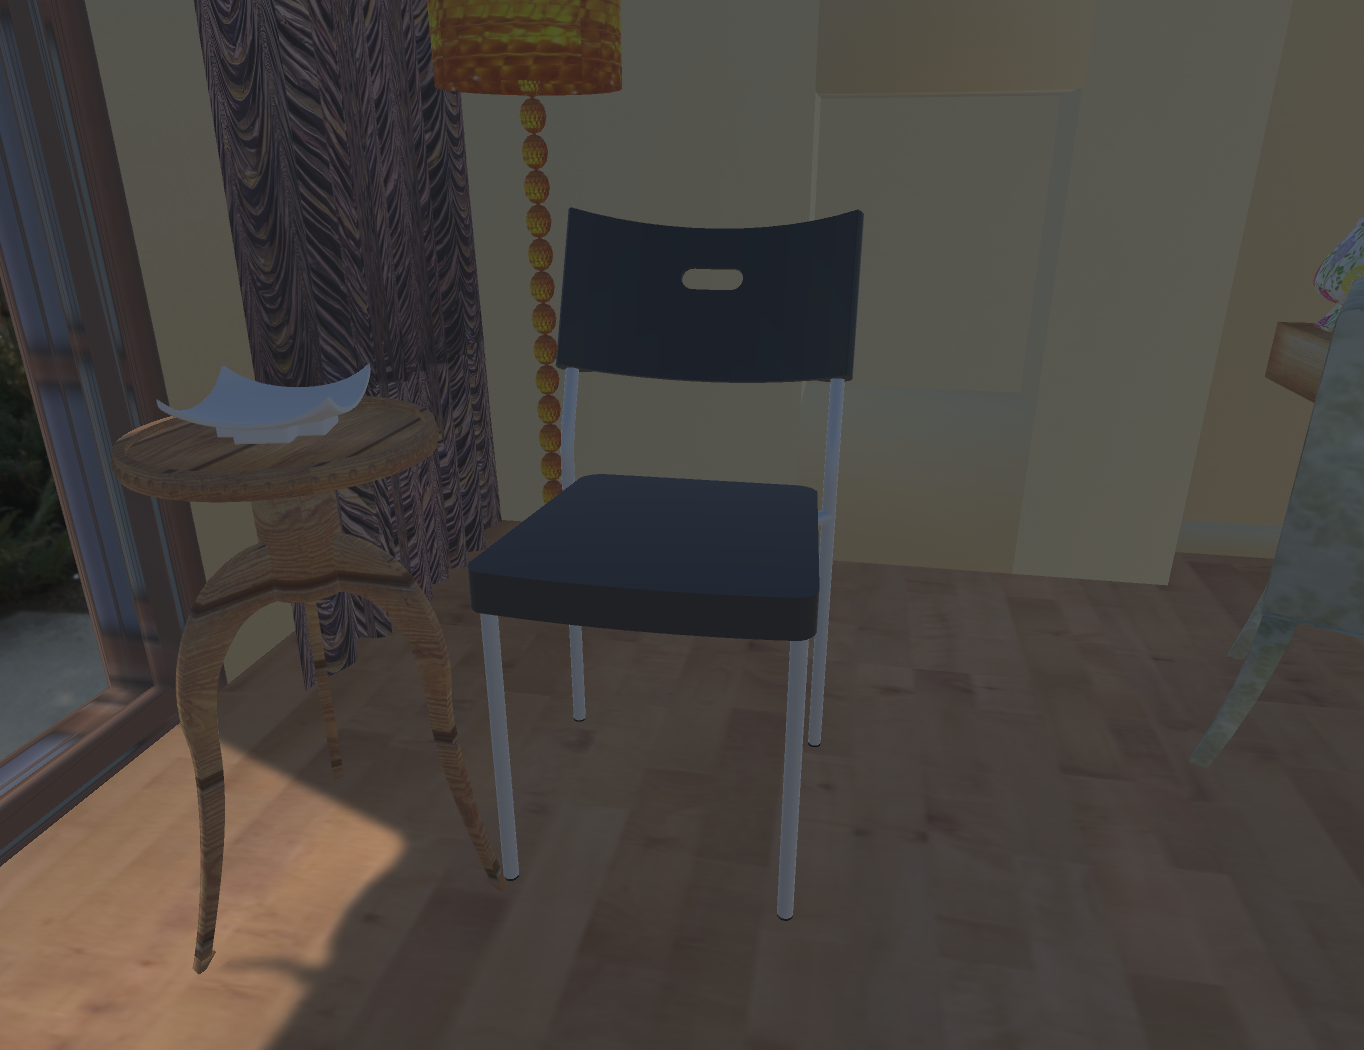
\includegraphics[width=.19\linewidth]{/Users/apple/OVGU/Thesis/code/3dReconstruction/report/images/implementation/gbuffers/0_img}
        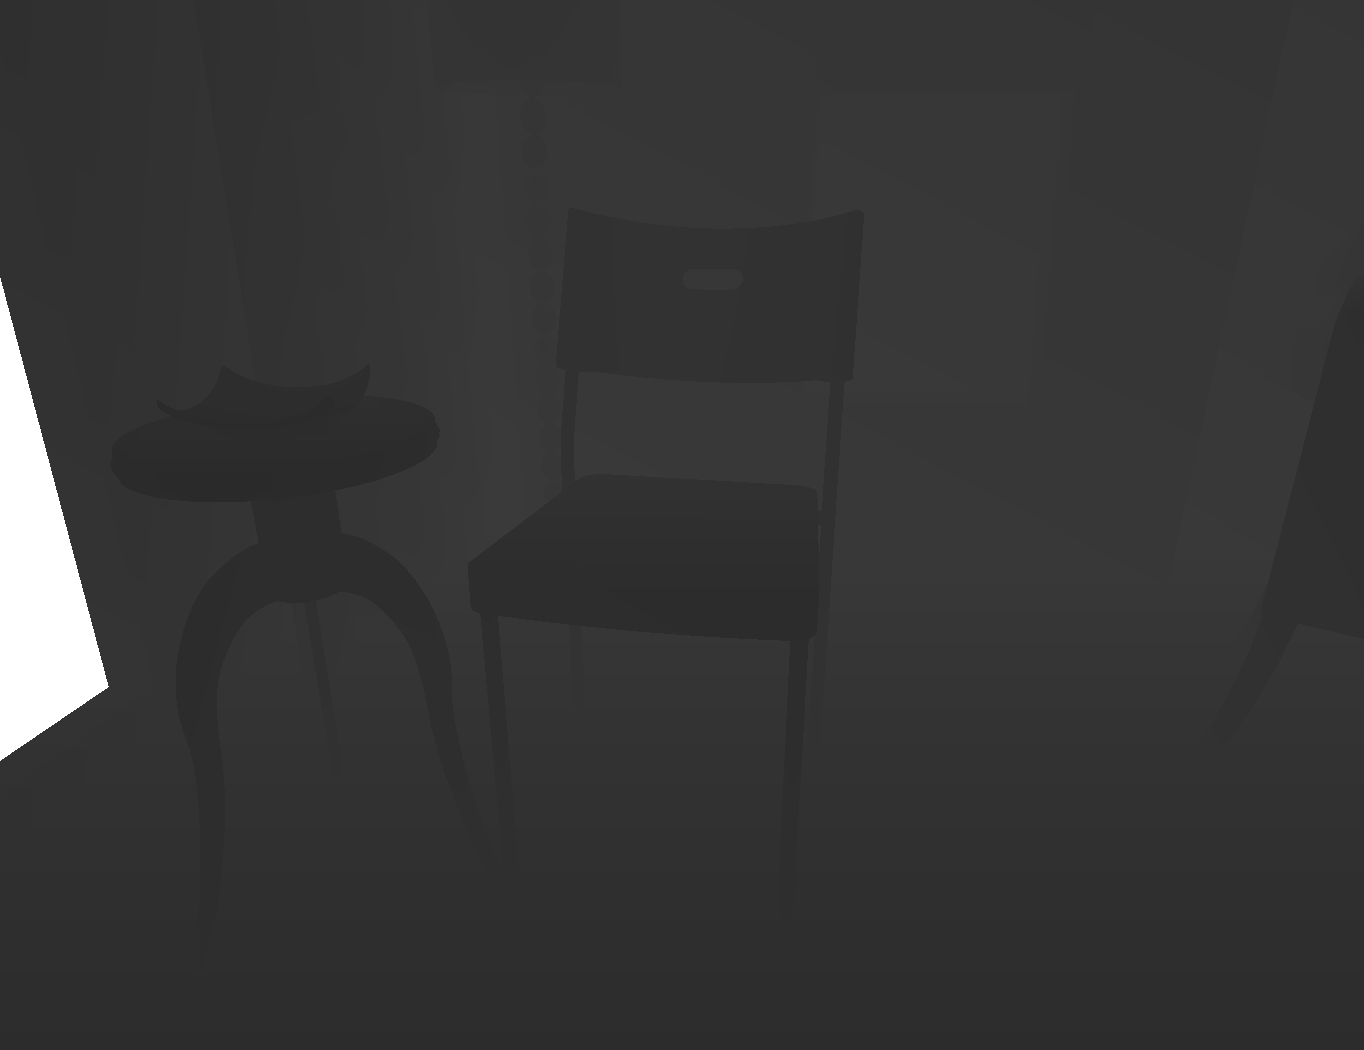
\includegraphics[width=.19\linewidth]{/Users/apple/OVGU/Thesis/code/3dReconstruction/report/images/implementation/gbuffers/0_depth}
        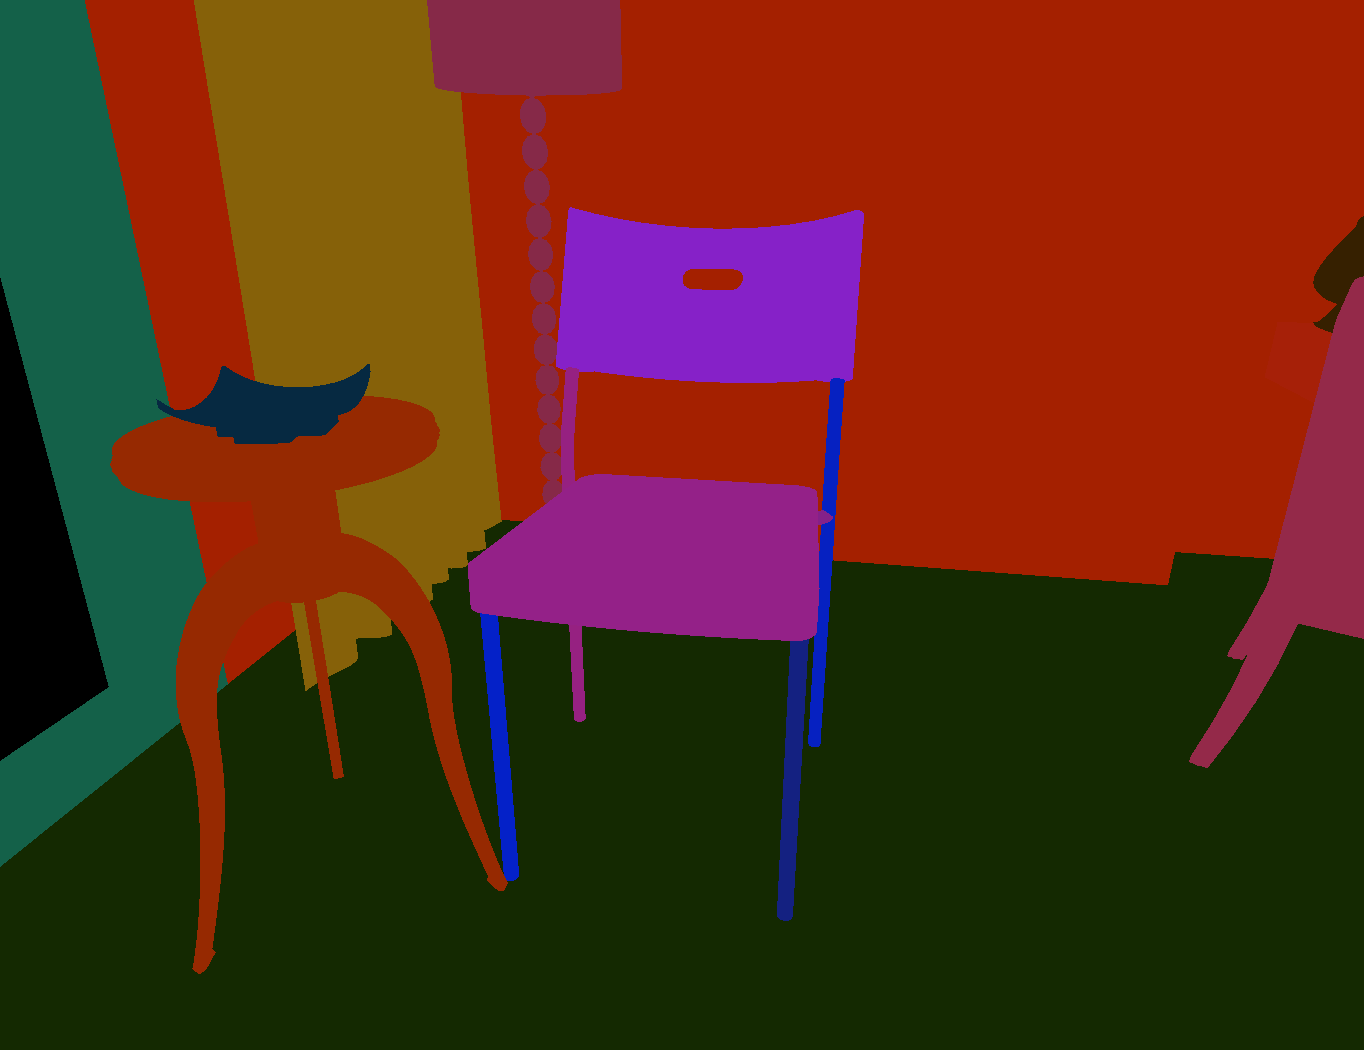
\includegraphics[width=.19\linewidth]{/Users/apple/OVGU/Thesis/code/3dReconstruction/report/images/implementation/gbuffers/0_id}
        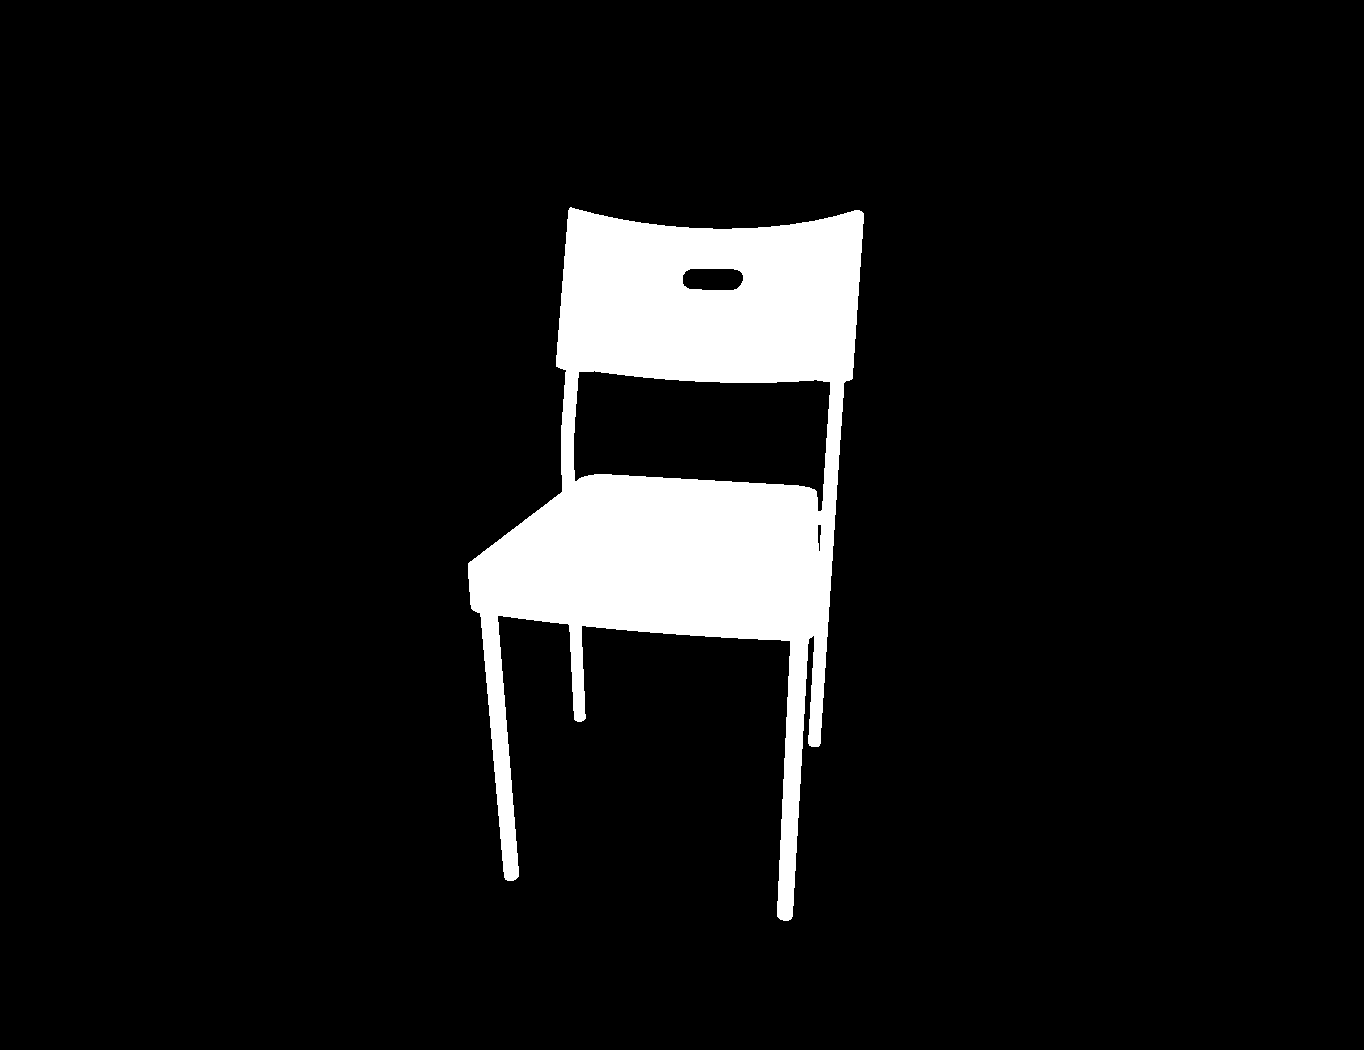
\includegraphics[width=.19\linewidth]{/Users/apple/OVGU/Thesis/code/3dReconstruction/report/images/implementation/gbuffers/0_layer}
        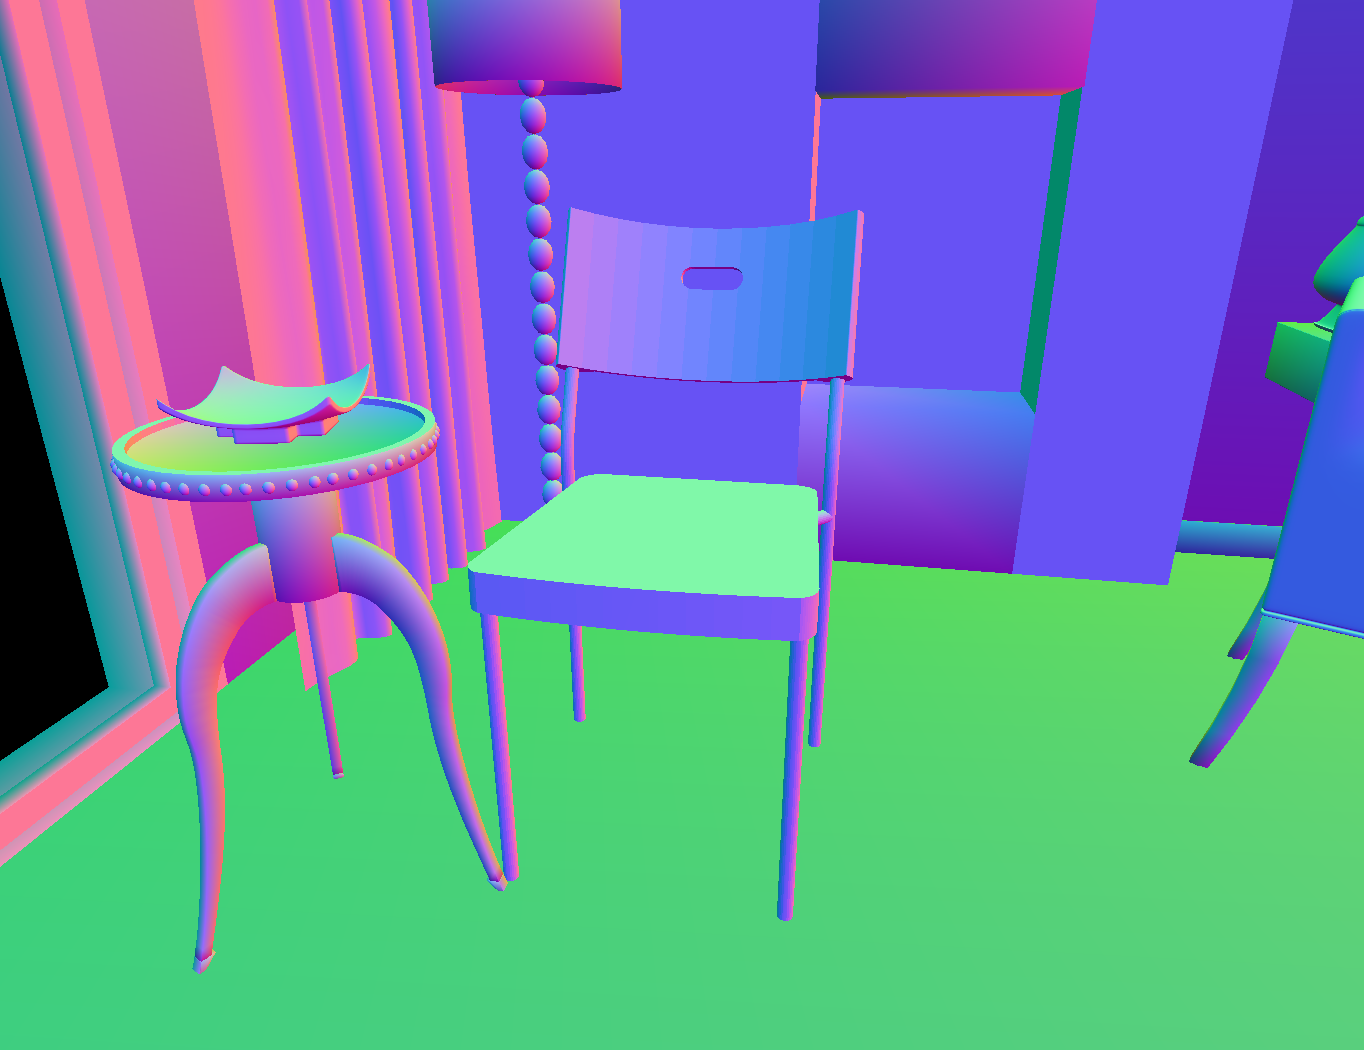
\includegraphics[width=.19\linewidth]{/Users/apple/OVGU/Thesis/code/3dReconstruction/report/images/implementation/gbuffers/0_normals}\\
        \vspace{0.1cm}
        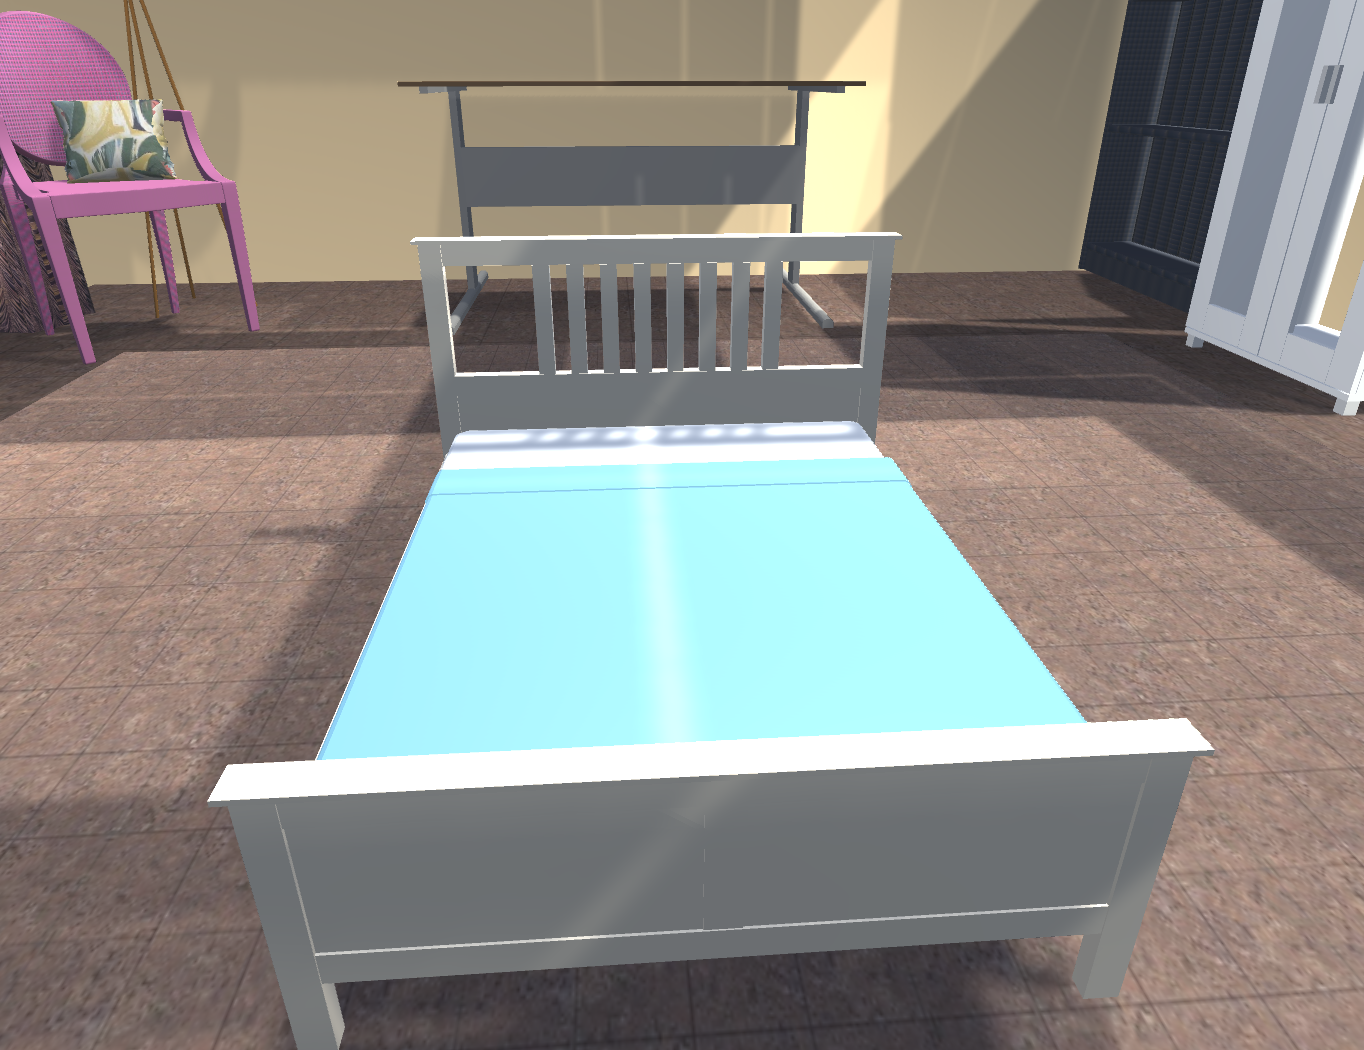
\includegraphics[width=.19\linewidth]{/Users/apple/OVGU/Thesis/code/3dReconstruction/report/images/implementation/gbuffers/1_img}
        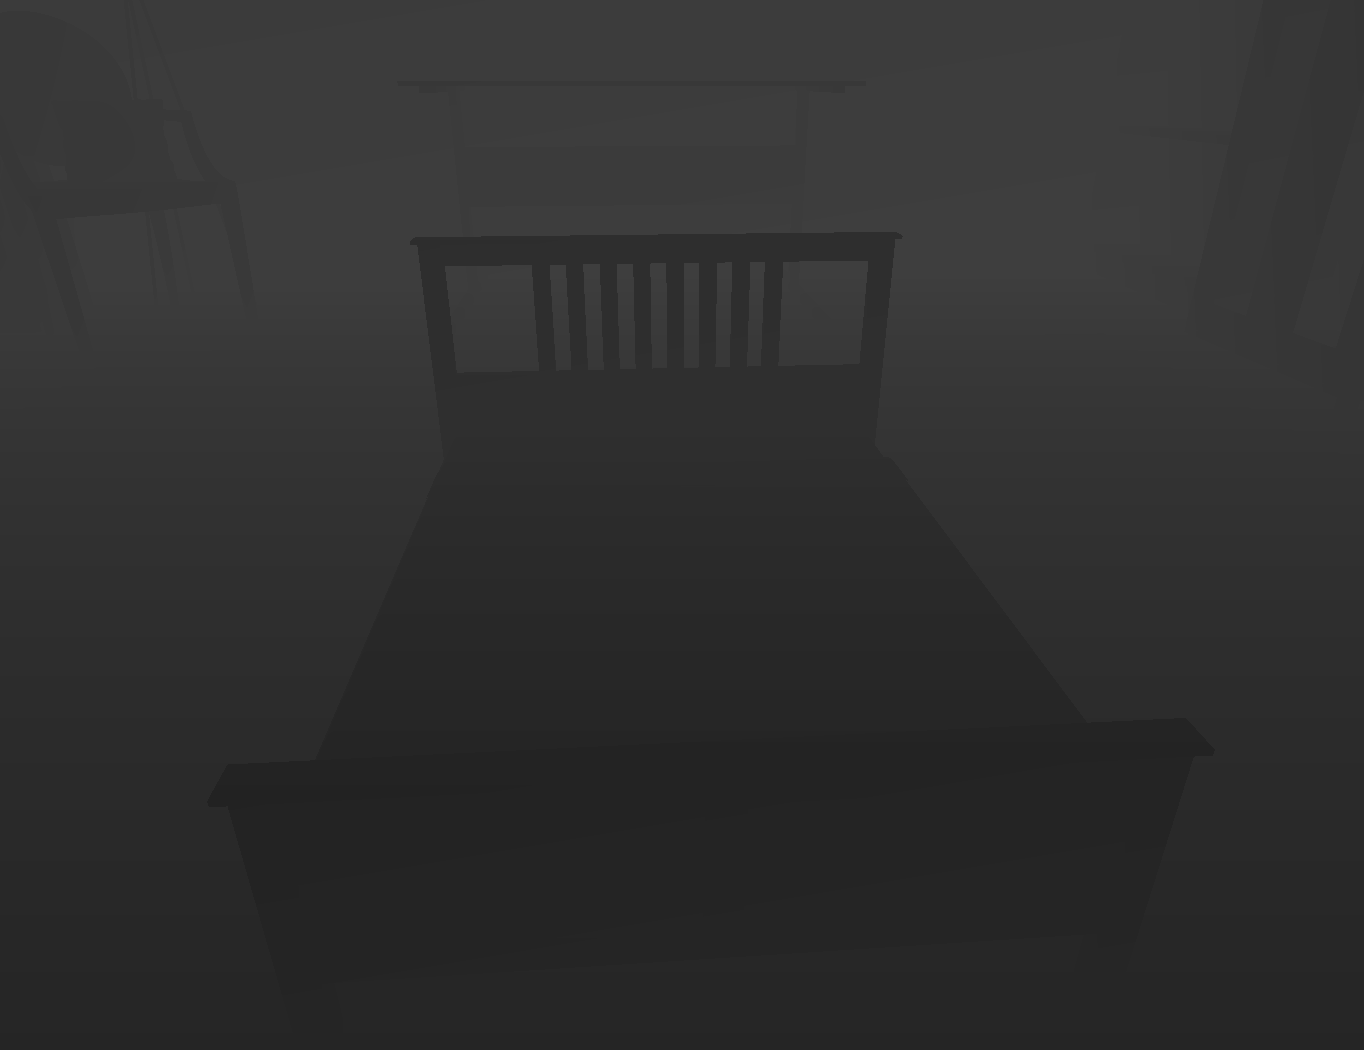
\includegraphics[width=.19\linewidth]{/Users/apple/OVGU/Thesis/code/3dReconstruction/report/images/implementation/gbuffers/1_depth}
        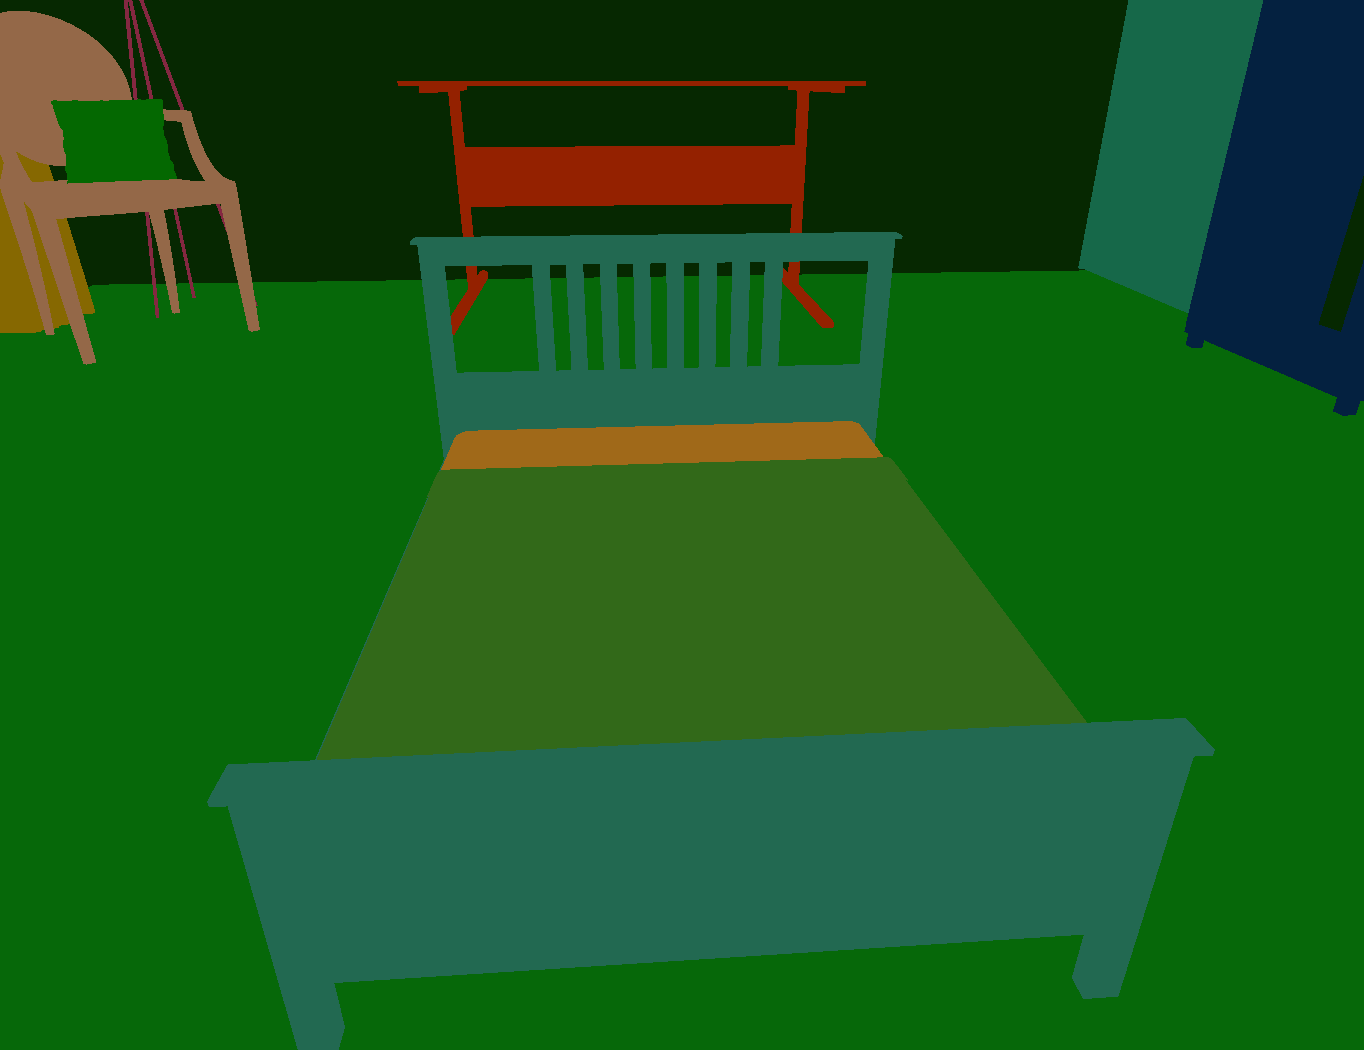
\includegraphics[width=.19\linewidth]{/Users/apple/OVGU/Thesis/code/3dReconstruction/report/images/implementation/gbuffers/1_id}
        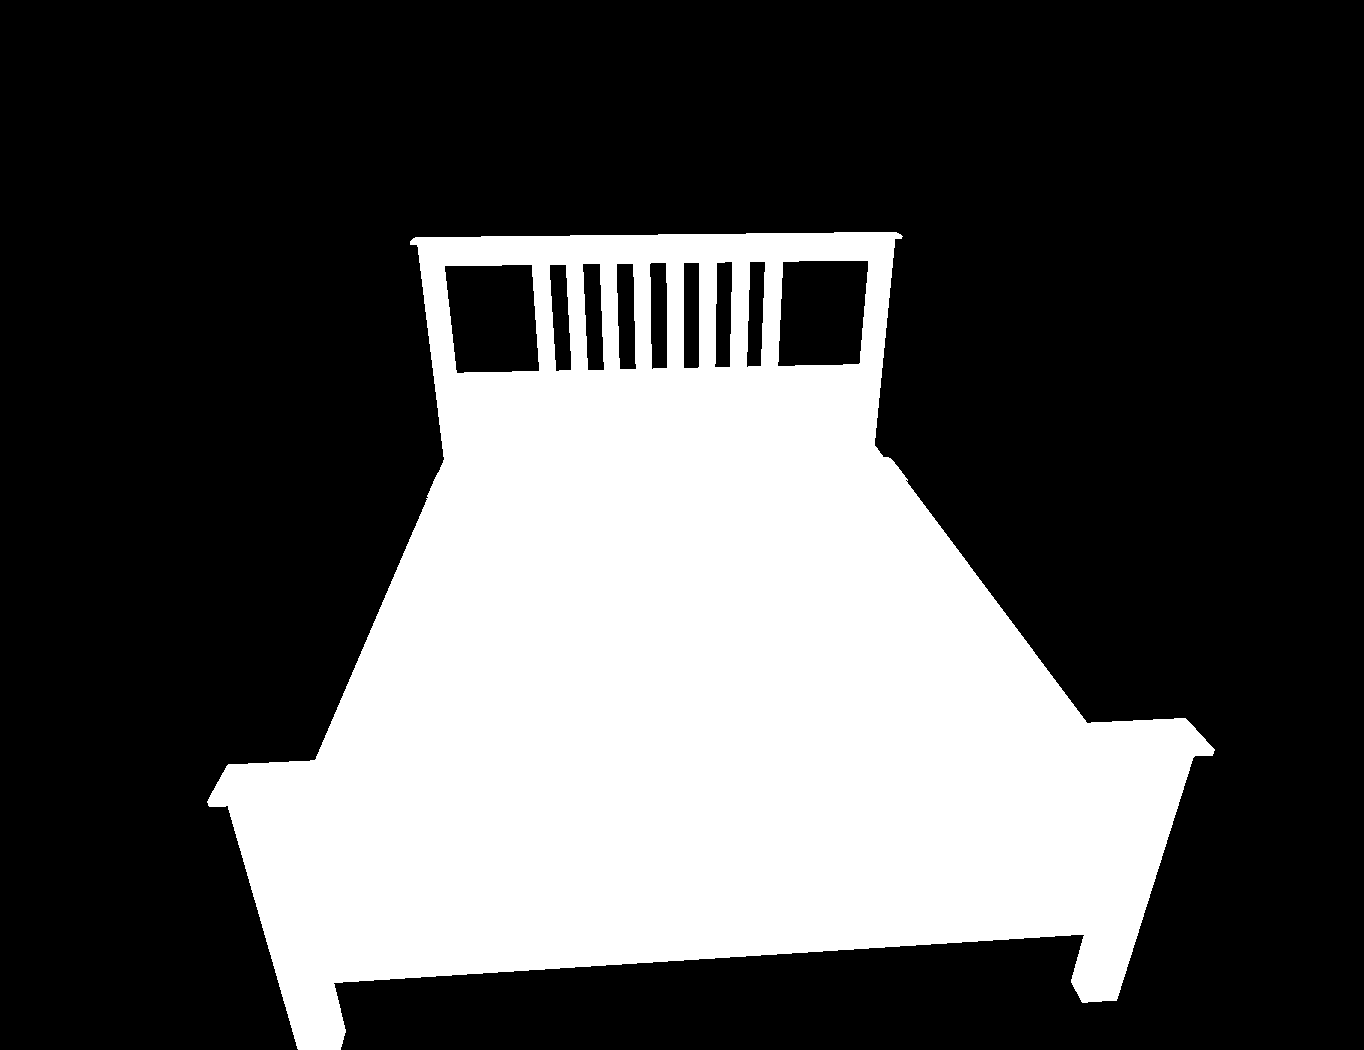
\includegraphics[width=.19\linewidth]{/Users/apple/OVGU/Thesis/code/3dReconstruction/report/images/implementation/gbuffers/1_layer}
        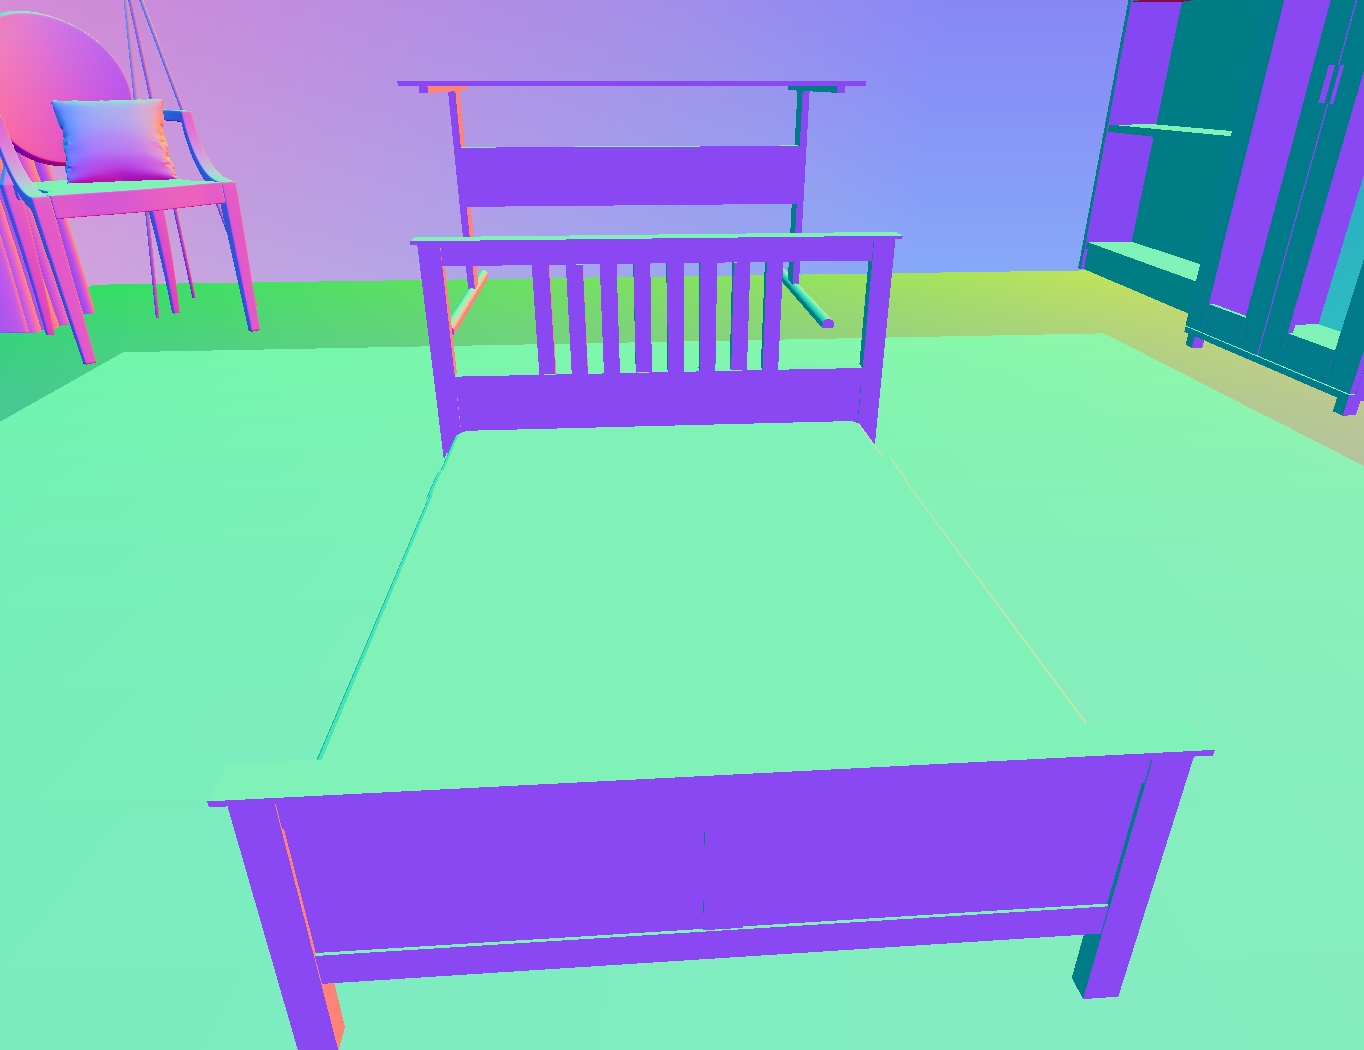
\includegraphics[width=.19\linewidth]{/Users/apple/OVGU/Thesis/code/3dReconstruction/report/images/implementation/gbuffers/1_normals}\\
        \vspace{0.1cm}

        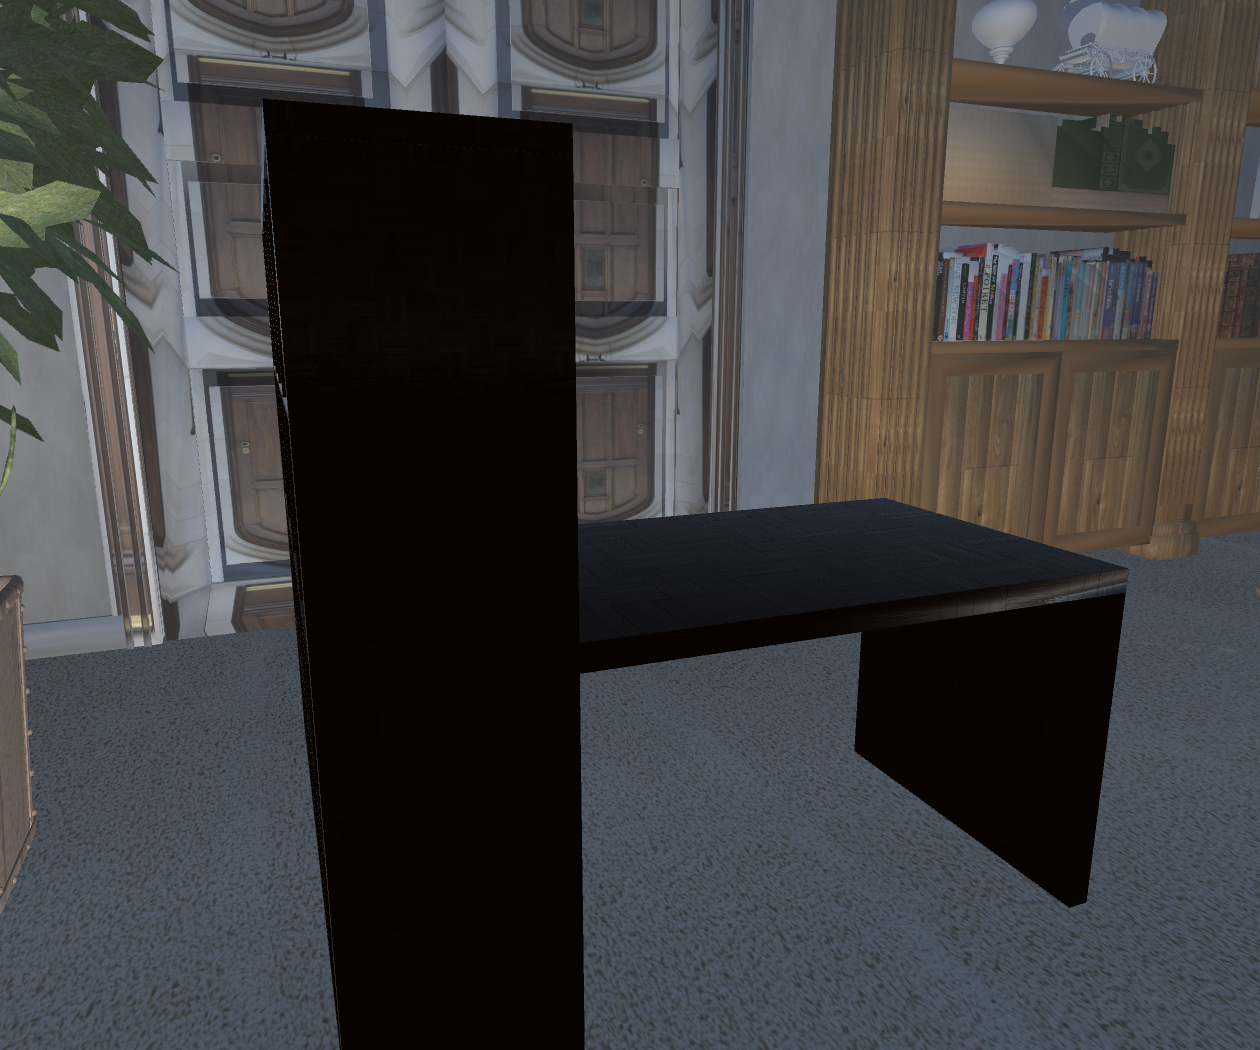
\includegraphics[width=.19\linewidth]{/Users/apple/OVGU/Thesis/code/3dReconstruction/report/images/implementation/gbuffers/2_img}
        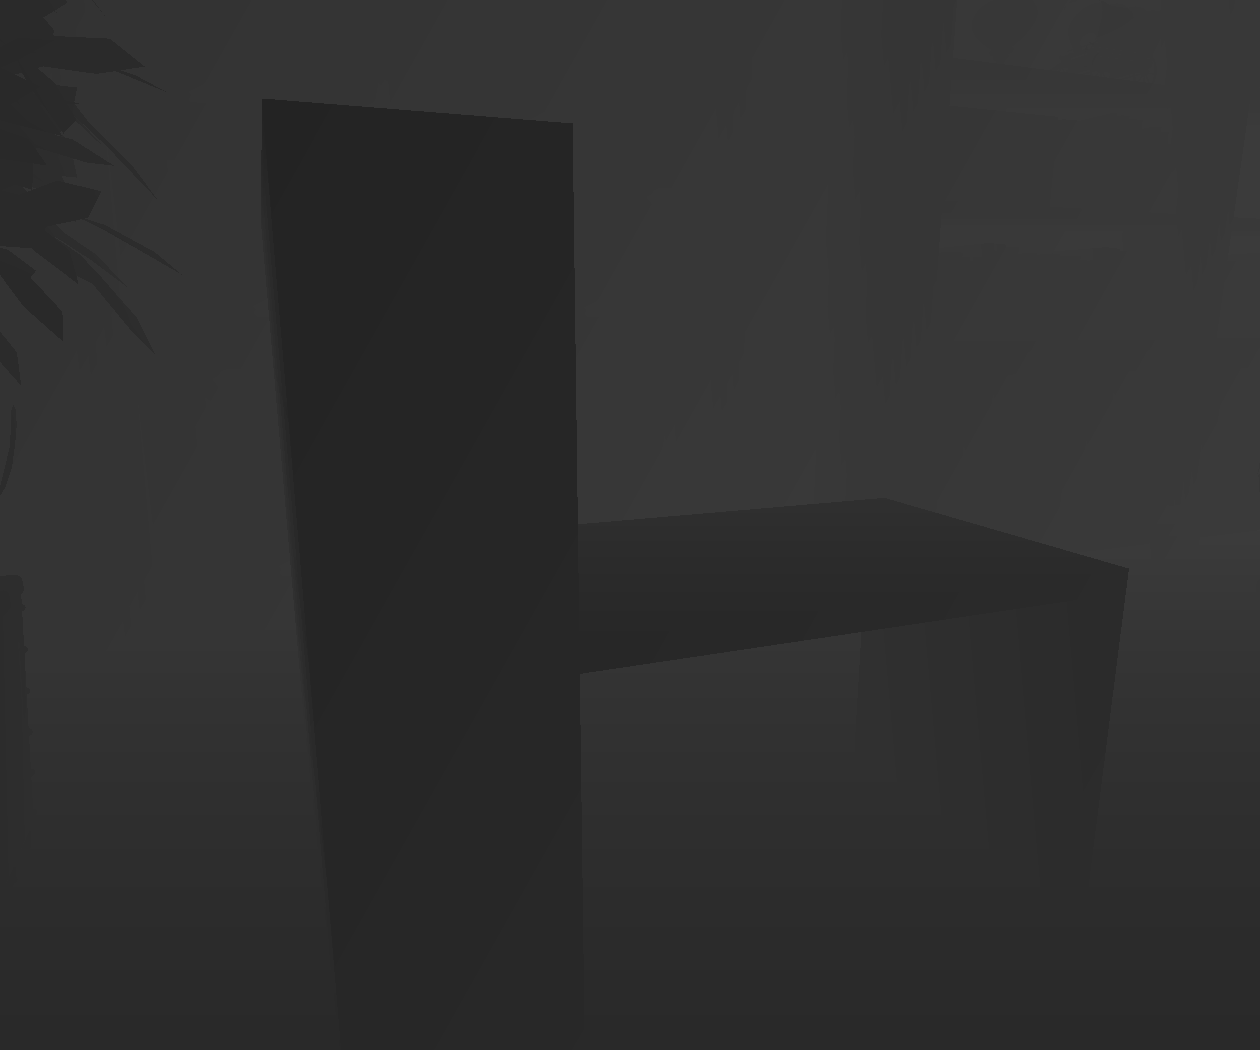
\includegraphics[width=.19\linewidth]{/Users/apple/OVGU/Thesis/code/3dReconstruction/report/images/implementation/gbuffers/2_depth}
        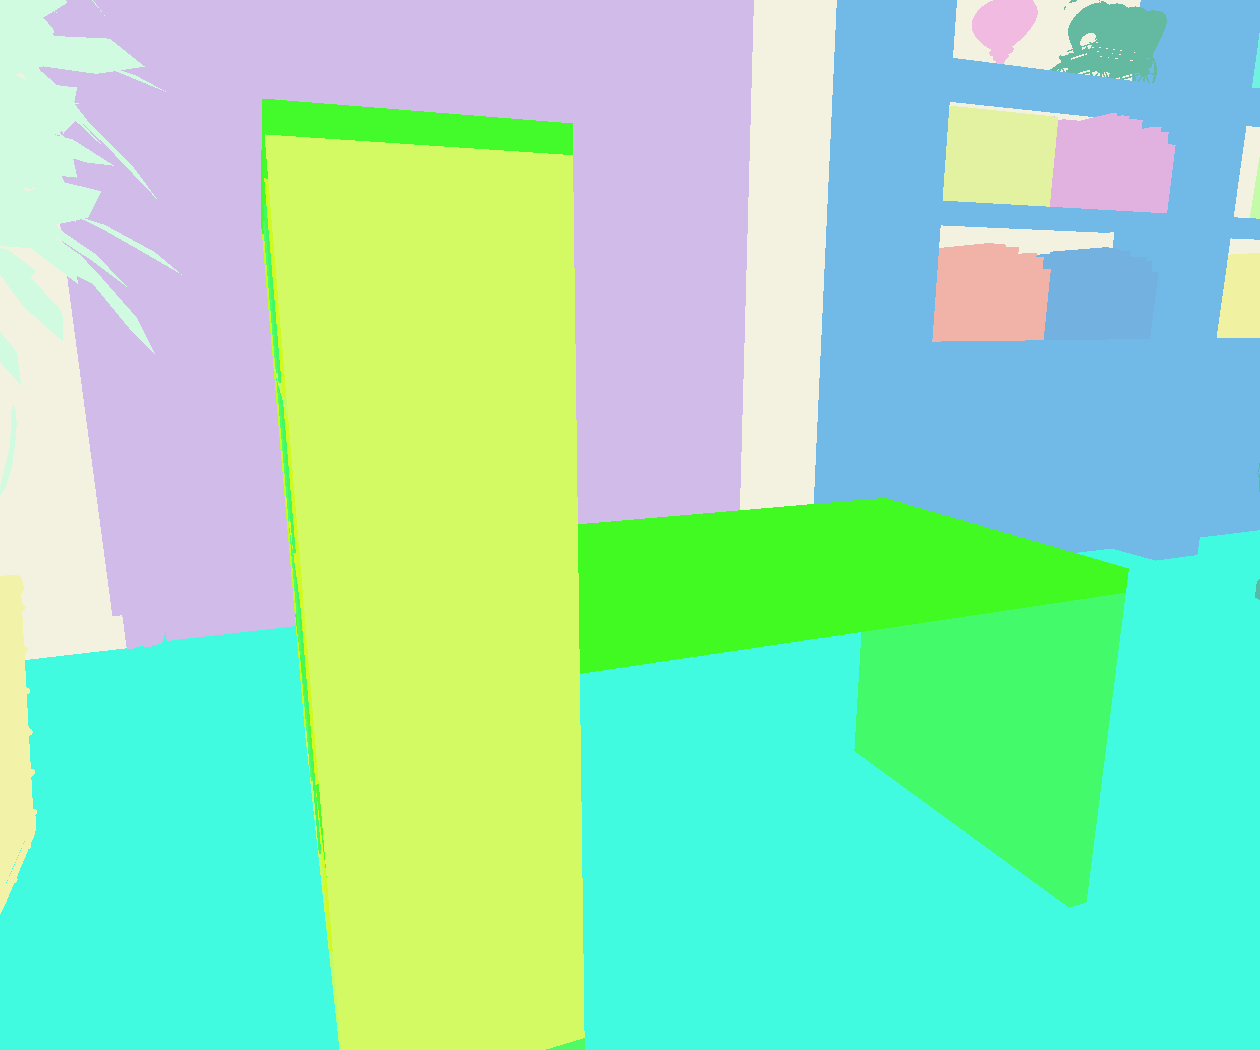
\includegraphics[width=.19\linewidth]{/Users/apple/OVGU/Thesis/code/3dReconstruction/report/images/implementation/gbuffers/2_id}
        
\includegraphics[width=.19\linewidth]{/Users/apple/OVGU/Thesis/code/3dReconstruction/report/images/implementation/gbuffers/2_layer}
        \includegraphics[width=.19\linewidth]{/Users/apple/OVGU/Thesis/code/3dReconstruction/report/images/implementation/gbuffers/2_normals}\\
        \vspace{0.1cm}
        \includegraphics[width=.19\linewidth]{/Users/apple/OVGU/Thesis/code/3dReconstruction/report/images/implementation/gbuffers/3_img}
        \includegraphics[width=.19\linewidth]{/Users/apple/OVGU/Thesis/code/3dReconstruction/report/images/implementation/gbuffers/3_depth}
        \includegraphics[width=.19\linewidth]{/Users/apple/OVGU/Thesis/code/3dReconstruction/report/images/implementation/gbuffers/3_id}
        \includegraphics[width=.19\linewidth]{/Users/apple/OVGU/Thesis/code/3dReconstruction/report/images/implementation/gbuffers/3_layer}
        \includegraphics[width=.19\linewidth]{/Users/apple/OVGU/Thesis/code/3dReconstruction/report/images/implementation/gbuffers/3_normals}\\
    \vspace{0.1cm}

        \includegraphics[width=.19\linewidth]{/Users/apple/OVGU/Thesis/code/3dReconstruction/report/images/implementation/gbuffers/4_img}
        \includegraphics[width=.19\linewidth]{/Users/apple/OVGU/Thesis/code/3dReconstruction/report/images/implementation/gbuffers/4_depth}
        \includegraphics[width=.19\linewidth]{/Users/apple/OVGU/Thesis/code/3dReconstruction/report/images/implementation/gbuffers/4_id}
        \includegraphics[width=.19\linewidth]{/Users/apple/OVGU/Thesis/code/3dReconstruction/report/images/implementation/gbuffers/4_layer}
        \includegraphics[width=.19\linewidth]{/Users/apple/OVGU/Thesis/code/3dReconstruction/report/images/implementation/gbuffers/4_normals}\\
    \vspace{0.1cm}

        \includegraphics[width=.19\linewidth]{/Users/apple/OVGU/Thesis/code/3dReconstruction/report/images/implementation/gbuffers/5_img}
        \includegraphics[width=.19\linewidth]{/Users/apple/OVGU/Thesis/code/3dReconstruction/report/images/implementation/gbuffers/5_depth}
        \includegraphics[width=.19\linewidth]{/Users/apple/OVGU/Thesis/code/3dReconstruction/report/images/implementation/gbuffers/5_id}
        \includegraphics[width=.19\linewidth]{/Users/apple/OVGU/Thesis/code/3dReconstruction/report/images/implementation/gbuffers/5_layer}
        \includegraphics[width=.19\linewidth]{/Users/apple/OVGU/Thesis/code/3dReconstruction/report/images/implementation/gbuffers/5_normals}\\
    \vspace{0.1cm}

        \includegraphics[width=.19\linewidth]{/Users/apple/OVGU/Thesis/code/3dReconstruction/report/images/implementation/gbuffers/6_img}
        \includegraphics[width=.19\linewidth]{/Users/apple/OVGU/Thesis/code/3dReconstruction/report/images/implementation/gbuffers/6_depth}
        \includegraphics[width=.19\linewidth]{/Users/apple/OVGU/Thesis/code/3dReconstruction/report/images/implementation/gbuffers/6_id}
        \includegraphics[width=.19\linewidth]{/Users/apple/OVGU/Thesis/code/3dReconstruction/report/images/implementation/gbuffers/6_layer}
        \includegraphics[width=.19\linewidth]{/Users/apple/OVGU/Thesis/code/3dReconstruction/report/images/implementation/gbuffers/6_normals}\\
    \caption{Samples for G-buffers collected from ImageSynthesis as part of the dataset. In the figure,
        (From left to right) RGB image, Depth map, Instance segmentation, Semantic Segmentation and Normal map}
    \label{fig:G-buffers samples}
\end{figure}


Replacing models, lighting(indoor and outdoor), randomisation of texture, camera distance, camera angles, outdoor skybox,
UI controls
Manual inputs, automated
Unity - ML-ImageSynthesis
UML diagram is needed? (If it helps)

\section{3d-Reconstruction framework}\label{s:3D-Reconstruction framework}


Development environment
Training setup(hardware, voxel size…)
Mixed precision using apex
If mixed precision helped performance, memory, speed, evaluation metric


%\section{Implement a domain adaptation technique}{}
%To serve as a proof if more domain gap reduction is needed.
